\documentclass[a4paper]{article}
\usepackage[colorlinks,linkcolor=black,urlcolor=black]{hyperref}
\usepackage{float}
\usepackage{mhchem}
\usepackage{pdfpages}
\usepackage{enumerate}
\usepackage{amsmath}
\usepackage{amssymb}
\usepackage{graphicx}
\usepackage{subfigure}
\usepackage{wrapfig}
\usepackage{geometry}
\usepackage{indentfirst}
\usepackage{array}
\usepackage{multirow} 
\usepackage{verbatim}
\setlength{\parindent}{2em}
\usepackage[greek,english]{babel} 
\geometry{left=2cm,right=2cm,top=1.5cm,bottom=1.5cm}

\begin{document}

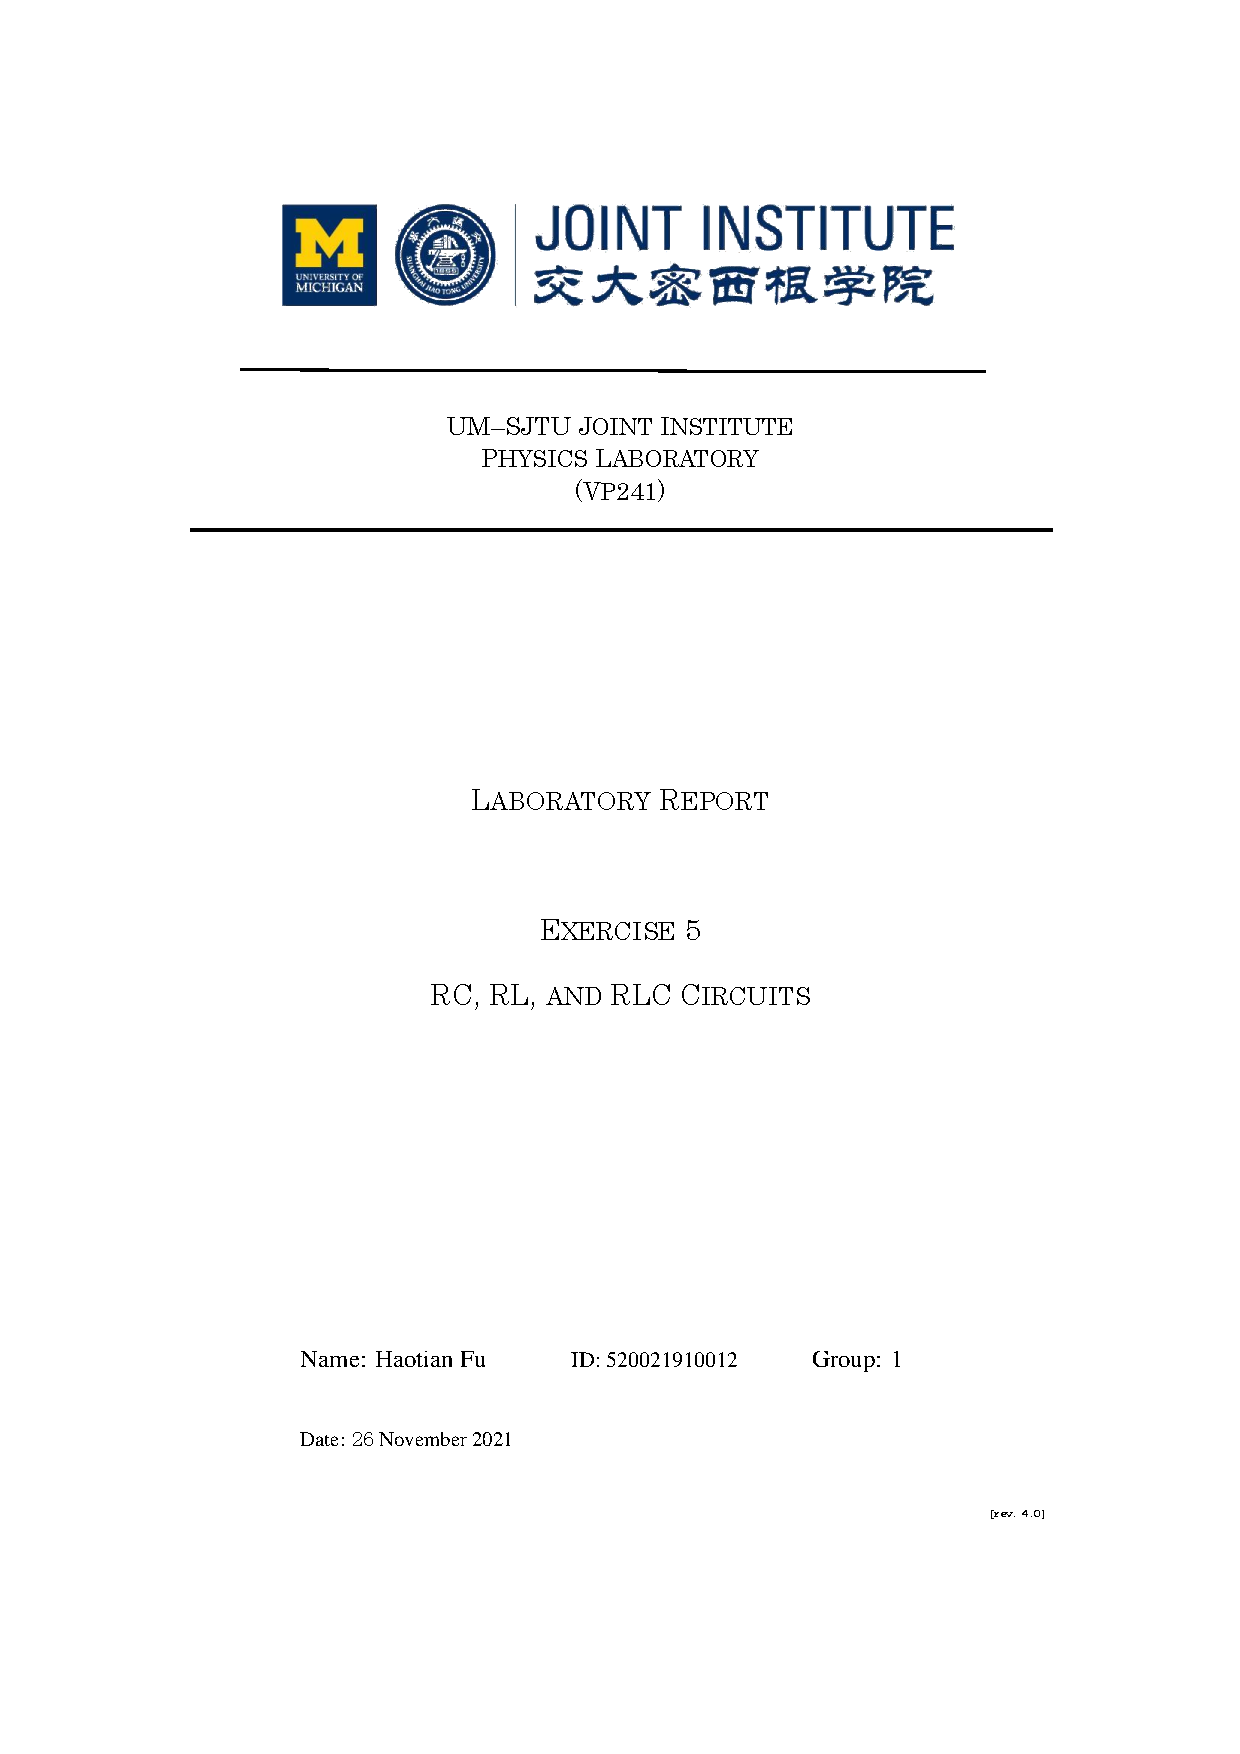
\includepdf{lab5_cover.pdf}

\newpage
\tableofcontents
\setcounter{page}{1}

\newpage
\listoffigures
\listoftables

\newpage
\section{Introduction}

The objective of this exercise is to help students understand the physics of alternating-current circuits, in specific processes of charging/discharging of capacitors, the phenomenon of electromagnetic induction in inductive elements, and other dynamic processes in $RC$, $RL$, and $RLC$ series circuits.

In this exercise, students will study methods for measuring the amplitude-frequency and the phase-frequency characteristics of $RC$, $RL$, and $RLC$ series circuits.  The resonance frequency of an $RLC$ circuit as well as the quality factor of the circuit will be found from the amplitude-frequency curve.

\subsection{Basic Concepts}
\begin{itemize}
	\item \textbf{Alternating current(AC)}$^{[1]}$

	      Alternating current(AC) is an electric current which periodically reverses direction.

	\item \textbf{Transient Process}$^{[2]}$

	      In a $RC$ circuit, the process of charging or discharging of the capacitor is an example of a transient process.

	\item \textbf{Half-life}$^{[2]}$

	      The half-life period is the time needed for $U_C$ to decrease a half of the initial value (or increase to a half of the terminal value), and may be also used to characterize the dynamics of the transient process.

	\item \textbf{Resonance}$^{[3]}$

	      Electrical resonance occurs in an electric circuit at a particular resonant frequency when the impedance of the circuit is at a minimum in a series circuit or at maximum in a parallel circuit (or when the transfer function is at a maximum).
\end{itemize}

\subsection{Transient Processes in $RC$, $RL$, $RLC$ Series Circuits}

\subsubsection{$RC$ Series Circuit}

\begin{figure}[!htbp]
	\center
	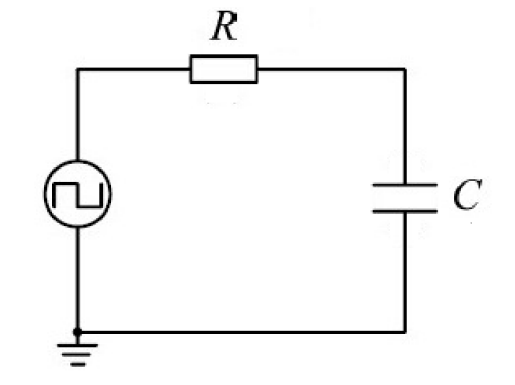
\includegraphics[width=0.4\textwidth]{RC_series_circuit.png}
	\caption{$RC$ series circuit}
	\label{fig::RC_series}
\end{figure}

In a $RC$ circuit, the process of charging or discharging of the capacitor is an example of a transient process. Figure 1 shows a RC series circuit in which a square-wave signal is used as the source signal. In the first half of the cycle, the square-wave voltage is $U(t) = \mathcal{E}$ and it charges the capacitor. In the second half-cycle, the square-wave voltage is zero, and the capacitor discharges through the resistor.

The loop equation (Kirchhoff’s loop rule) for the charging process is
\begin{equation}
	RC\frac{dU_c}{dt}+U_c=\mathcal{E}
	\label{eq::Kirchoff}
\end{equation}

With the initial condition $U_C(t = 0) = 0$, the solution of Eq.(\ref{eq::Kirchoff}) can be found as
$$U_C=\mathcal{E}(1-e^{-\frac{t}{RC}})$$
$$U_R=iR=\mathcal{E} e^{-\frac{t}{RC}}$$

Hence the voltage across the capacitor $U_C$ increases exponentially with time $t$, whereas the voltage on the resistor $U_R$ decreases exponentially with time. The curves $U(t)$, $U_C(t),$ and $U_R(t)$ are shown in Fig. \ref{fig::charging_discharging}.

\begin{figure}[!htbp]
	\center
	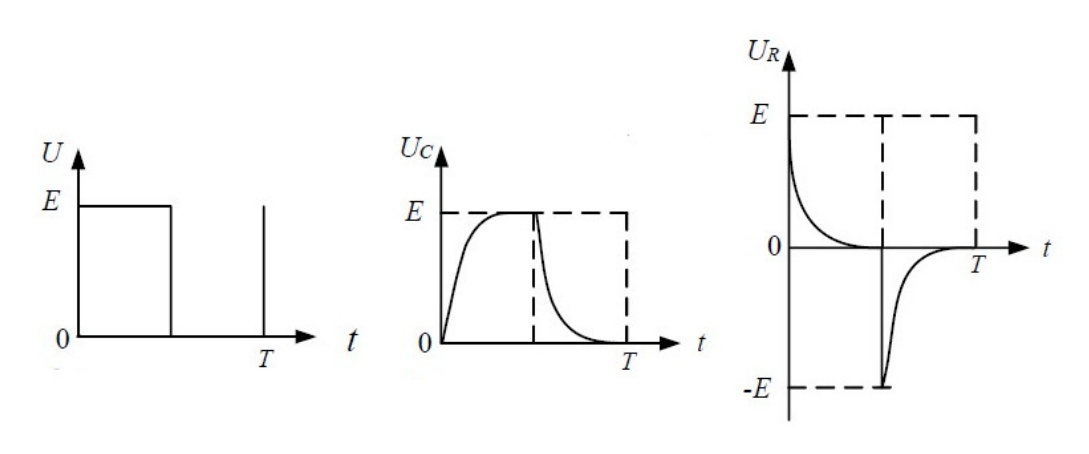
\includegraphics[width=0.8\textwidth]{charging_discharing.png}
	\caption{Charging/discharging curves for a $RC$ series circuit}
	\label{fig::charging_discharging}
\end{figure}

For the discharging process, the loop rule gives
\begin{equation}
	RC\frac{dU_C}{dt}+U_C=0
\end{equation}

The solution of Eq. (2), with the initial condition $U_C(t=0)=\varepsilon$, is
$$U_C=\mathcal{E} e^{-\frac{t}{RC}}$$
and, consequently,
$$U_R=iR=-\mathcal{E} e^{-\frac{t}{RC}}$$
where the magnitudes of both $U_C$ and $U_R$ decrease exponentially with time.

Since $RC = \tau$ has the units of time, it is called the time constant of the circuit, and characterizes the dynamics of the transient process. There is another characteristics related to the time constant, easier to measure in experiments, which is called the half-life period $T_{1/2}$. The half-life period is the time needed for $U_C$ to decrease a half of the initial value (or increase to a half of the terminal value), and may be also used to characterize the dynamics of the transient process. Both quantities, in the process with exponential dynamics discussed above, are related by the equation
$$T_{1/2}=\tau\ln2\approx0.693\tau.$$

\subsubsection{RL Series Circuit}

A similar analysis can be carried out for a RL series circuit. In this case
$$\tau=\frac{L}{R}\qquad \mathrm{and}\qquad T_{1/2}=\frac{L}{R}\ln2$$

\subsubsection{RLC Series Circuit}

First, we discuss the situation when a power source is suddenly plugged into a $RLC$ circuit. Then the voltage across the capacitor satisfies the differential equation
\begin{equation}
	LC\frac{d^2U_C}{dt^2}+RC\frac{dU_C}{dt}+U_C=\mathcal{E}
	\label{eq::differential}
\end{equation}
following again from the loop rule. Dividing both sides of the equation by $LC$ and introducing the symbols
$$
	\beta=\frac{R}{2L}\qquad \mathrm{and} \qquad \omega_0=\frac{1}{\sqrt{LC}}
$$
Eq.(\ref{eq::differential}) can be rewritten as
\begin{equation}
	\frac{d^2U_C}{dt^2}+2\beta\frac{dU_C}{dt}+\omega_0^2U_C=\omega_0^2\mathcal{E}
	\label{eq::differential_simplified}
\end{equation}

Note that Eq.(\ref{eq::differential_simplified}) is an inhomogeneous differential equation and it is mathematically equivalent to the equation of motion of a damped harmonic oscillator with a constant driving force. Therefore, the complementary homogeneous equation is fully analogous to the equation of motion of a damped harmonic oscillator, with $\beta$ being the damping coefficient, and $\omega_0$ — the natural angular frequency. Moreover, after a specific solution to the inhomogeneous equation is found, a unique solution to the initial value problem consisting of Eq.5 and the initial conditions
\begin{equation}
	U_C(t=0)=0\qquad \text{and} \qquad \left.\frac{dU_C}{dt}\right|_{t=0}=0
\end{equation}
can be found.

Exactly as for mechanical oscillations, depending on the relation between $\beta$ and $\omega_0$, there are three regimes, as implied by the solution of the complementary homogeneous equation:

\begin{enumerate}[i)]
	\item If $\beta^2 -\omega^2_0 < 0$ (weak damping), the system is in the under-damped regime and the solution to the initial value problem is of the form
	      $$U_C=\mathcal{E}-\mathcal{E} e^{-\beta t}\left(\cos\omega t+\frac{\beta}{\omega}\sin\omega t\right)$$
	      where $\omega=\sqrt{\omega^2_0-\beta^2}$

	\item If $\beta^2 -\omega^2_0 > 0$ (strong damping), the system is in the over-damped regime with the solution of the form
	      $$U_C=\mathcal{E}-\frac{\mathcal{E}}{2\gamma}e^{-\beta t}[(\beta+\gamma)e^{\gamma t}-(\beta-\gamma)e^{-\gamma t}]$$
	      where $\gamma=\sqrt{\beta^2-\omega^2}$

	\item Finally, if $\beta^2 -\omega^2_0 = 0$, the system is said to be critically damped, and
	      $$U_C=\mathcal{E}-\mathcal{E}(1+\beta t)e^{-\beta t}\eqno{(7)}$$
\end{enumerate}

When the circuit reaches a steady state, the power source is suddenly removed (E = 0). The differential equation for the discharging process is similar to that of the charging process, and there are also three regimes of the process.

The above discussion is valid for an ideal circuit and a step-signal source with zero internal resistance. In the experiment, the ideal system is replaced by a square-wave source with a small internal resistance. The period of the square-signal must be much greater than the time constant of the circuit. Note that, according to the above equations, the voltage across the capacitor $U_C$ will finally reach $\mathrm{E}$ regardless of the regime (Fig. \ref{fig::regimes}).

\begin{figure}[!htbp]
	\centering
	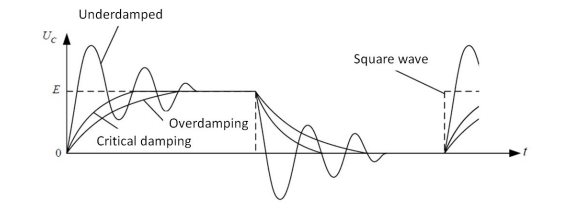
\includegraphics[width=12cm]{regimes.png}
	\caption{Three different regimes of transient processes in a RLC series circuit.}
	\label{fig::regimes}
\end{figure}

\subsection{RC, RL Steady-State Circuits}

When providing a sinusoidal alternating input voltageis provided to a RC (or RL) series circuit, the amplitude and the phase of the voltage across the capacitor and the resistor will change with the frequency of the input voltage. Then the amplitude vs. frequency relation and the phase vs. frequency relation can be obtained by measuring the voltage across the elements in the circuit for different input signal frequencies
$$\varphi = \tan^{-1}(\frac{U_L}{U_R}) = \tan^{-1}(\frac{\omega L}{R})$$
$$\varphi = \tan^{-1}(-\frac{U_C}{U_R}) = \tan^{-1}(-\frac{1}{\omega RC})$$
\subsection{RLC Resonant Circuit}
\subsubsection{RLC Series Circuit}
A generic $RLC$ series circuit is shown in Fig. \ref{fig::RLC}.

\begin{figure}[!htbp]
	\center
	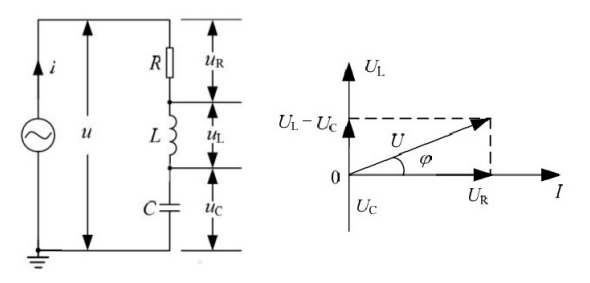
\includegraphics[width=10cm]{RLC.png}
	\caption{RLC series circuit}
	\label{fig::RLC}
\end{figure}

The impedance and the phase difference in the RLC circui can be calculated, e.g., by using the phasors technique. Representing the current $I$ by a vector along the horizontal axis, the phase differences between the current and the voltages across the resistor, coil, and capacitor are
$$\varphi_R=0,\qquad \varphi_L=\frac{\pi}{2},\qquad \varphi_C=-\frac{\pi}{2},$$
respectively. The corresponding voltage amplitudes across the elements are
$$U_R=IZ=IR, \qquad U_L=IZ_L=I\omega L, \qquad U_C=IZ_C=\frac{I}{\omega C}.$$
Hence, the voltage amplitude
$$U=\sqrt{U_R^2+(U_L-U_C)^2} \qquad \text{or} \qquad U=I\sqrt{R^2+(\omega L-\frac{1}{\omega C})^2}, \eqno{(8)}$$
and the total impedance
$$Z=\sqrt{R^2+(\omega L - \frac{1}{\omega C})^2},\eqno{(9)}$$
with the phase difference between the current and the voltage in the circuit
$$\varphi=\text{tan}^{-1}\frac{U_L-U_C}{U_R}=\text{tan}^{-1}\frac{\omega L-\frac{1}{\omega C}}{R}.$$

\subsubsection{Resonance}

If the frequency of the input signal provided by the source satisfies the condition
$$\omega_0 L = \frac{\omega_0}{C}, \hspace{2em} \Leftrightarrow \hspace{2em} \omega_0 = \frac{1}{\sqrt{LC}},$$
the total impedance will reach a minimum, $Z_0 = R$. Note that the resistance $R$ in a real circuit includes the internal resistance and all kinds of alternating-current power losses, so its actual value will be greater than the theoretical one.

When the current reaches its maximum, $I_m = U/R$, the circuit is said to be at resonance. The frequency
$$f_0 = \frac{\omega_0}{2\pi} = \frac{1}{2\pi\sqrt{LC}},$$
at which the resonance phenomenon occurs, is called the $\textit{resonance frequency}$.

The total impedance Z, current I, and the phase difference $\varphi=\varphi_u-\varphi_i$ all depend on frequency, with the generic shape of the curves shown in Figure 5. According to Eqs. (8) and (9), when the frequency is low($f<f_0,$ i.e. $1/\omega C>\omega L$), then $\varphi<0$. In this situation the total voltage lags behind the current and the circuit is said to be capacitive.

When the circuit is resonant($f=f_0$, i.e. $1/\omega C=\omega L$), then $\varphi<0$, the voltage across the capacitor and the inductor should be equal, and the circuit is said to be resistive.

Finally, when the frequency is high($f>f_0$, i.e. $\omega L > 1/\omega C$), and $\varphi>0$. In this situation the total voltage leads the current, and the circuit is said to be inductive.

\begin{figure}[!htbp]
	\centering
	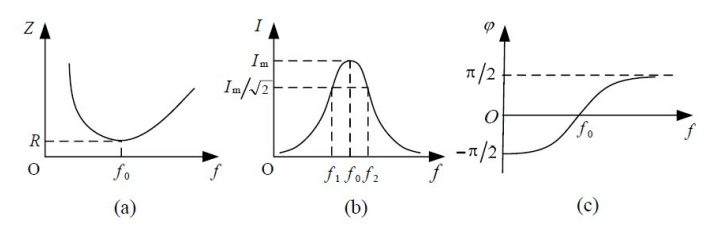
\includegraphics[width=15cm]{resonance.png}
	\caption{The impedance, the current and the phase difference as functions of the frequency for a $RLC$ series circuit (generic sketches)}
	\label{fig::resonance}
\end{figure}

\subsubsection{Quality Factor in Resonant Circuits}

Since $I_\text{m} = U/R$, the voltages across the resistor, the inductor, and the capacitor are
$$U_R = I_\text{m}R = U,$$
$$U_L = I_\text{m}Z_L = \frac{U}{R}\omega L,$$
$$U_C = I_\text{m}Z_C = \frac{U}{R}\frac{1}{\omega_0C} = U_L,$$
respectively. For a circuit driven at the resonance frequency, the ratio of $U_L$ (or $U_C$) to $U$ is called the quality factor $Q$ of a resonant circuit
$$Q = \frac{U_L}{U} = \frac{\omega_0 L}{R} \hspace{2em} \text{or} \hspace{2em} Q = \frac{U_C}{U} = \frac{1}{\omega_0 RC}.$$
When the total voltage is fixed, the greater $Q$ is, the greater $U_L$ and $U_C$ are. The value of $Q$ can be used to quantify the efficiency of resonant circuits.

The quality factor can also be found as
$$Q = \frac{f_0}{f_2 - f_1},$$
where $f_1$ and $f_2$ are two frequencies such that $I(f_1) = I(f_2) = I_\text{m}/\sqrt{2}$ (Fig. \ref{fig::resonance}).



\section{Apparatus and Measurement Procedure}

\subsection{Apparatus}

The apparatus involved in this lab include a signal generator, an oscilloscope, a digital multimeter, a wiring board, a fixed resistor 100 $\Omega$ (2 W), a variable resistor 2 $\text{k}\Omega$ (2 W), two capacitors 0.47 $\mu \text{F}$ and 0.1 $\mu\text{F}$, and two inductors (10 mH and 33 mH).

The following shows how to set up the apparatus. Remember to all black wires in one block to grounding.

\begin{figure}[!htbp]
	\centering
	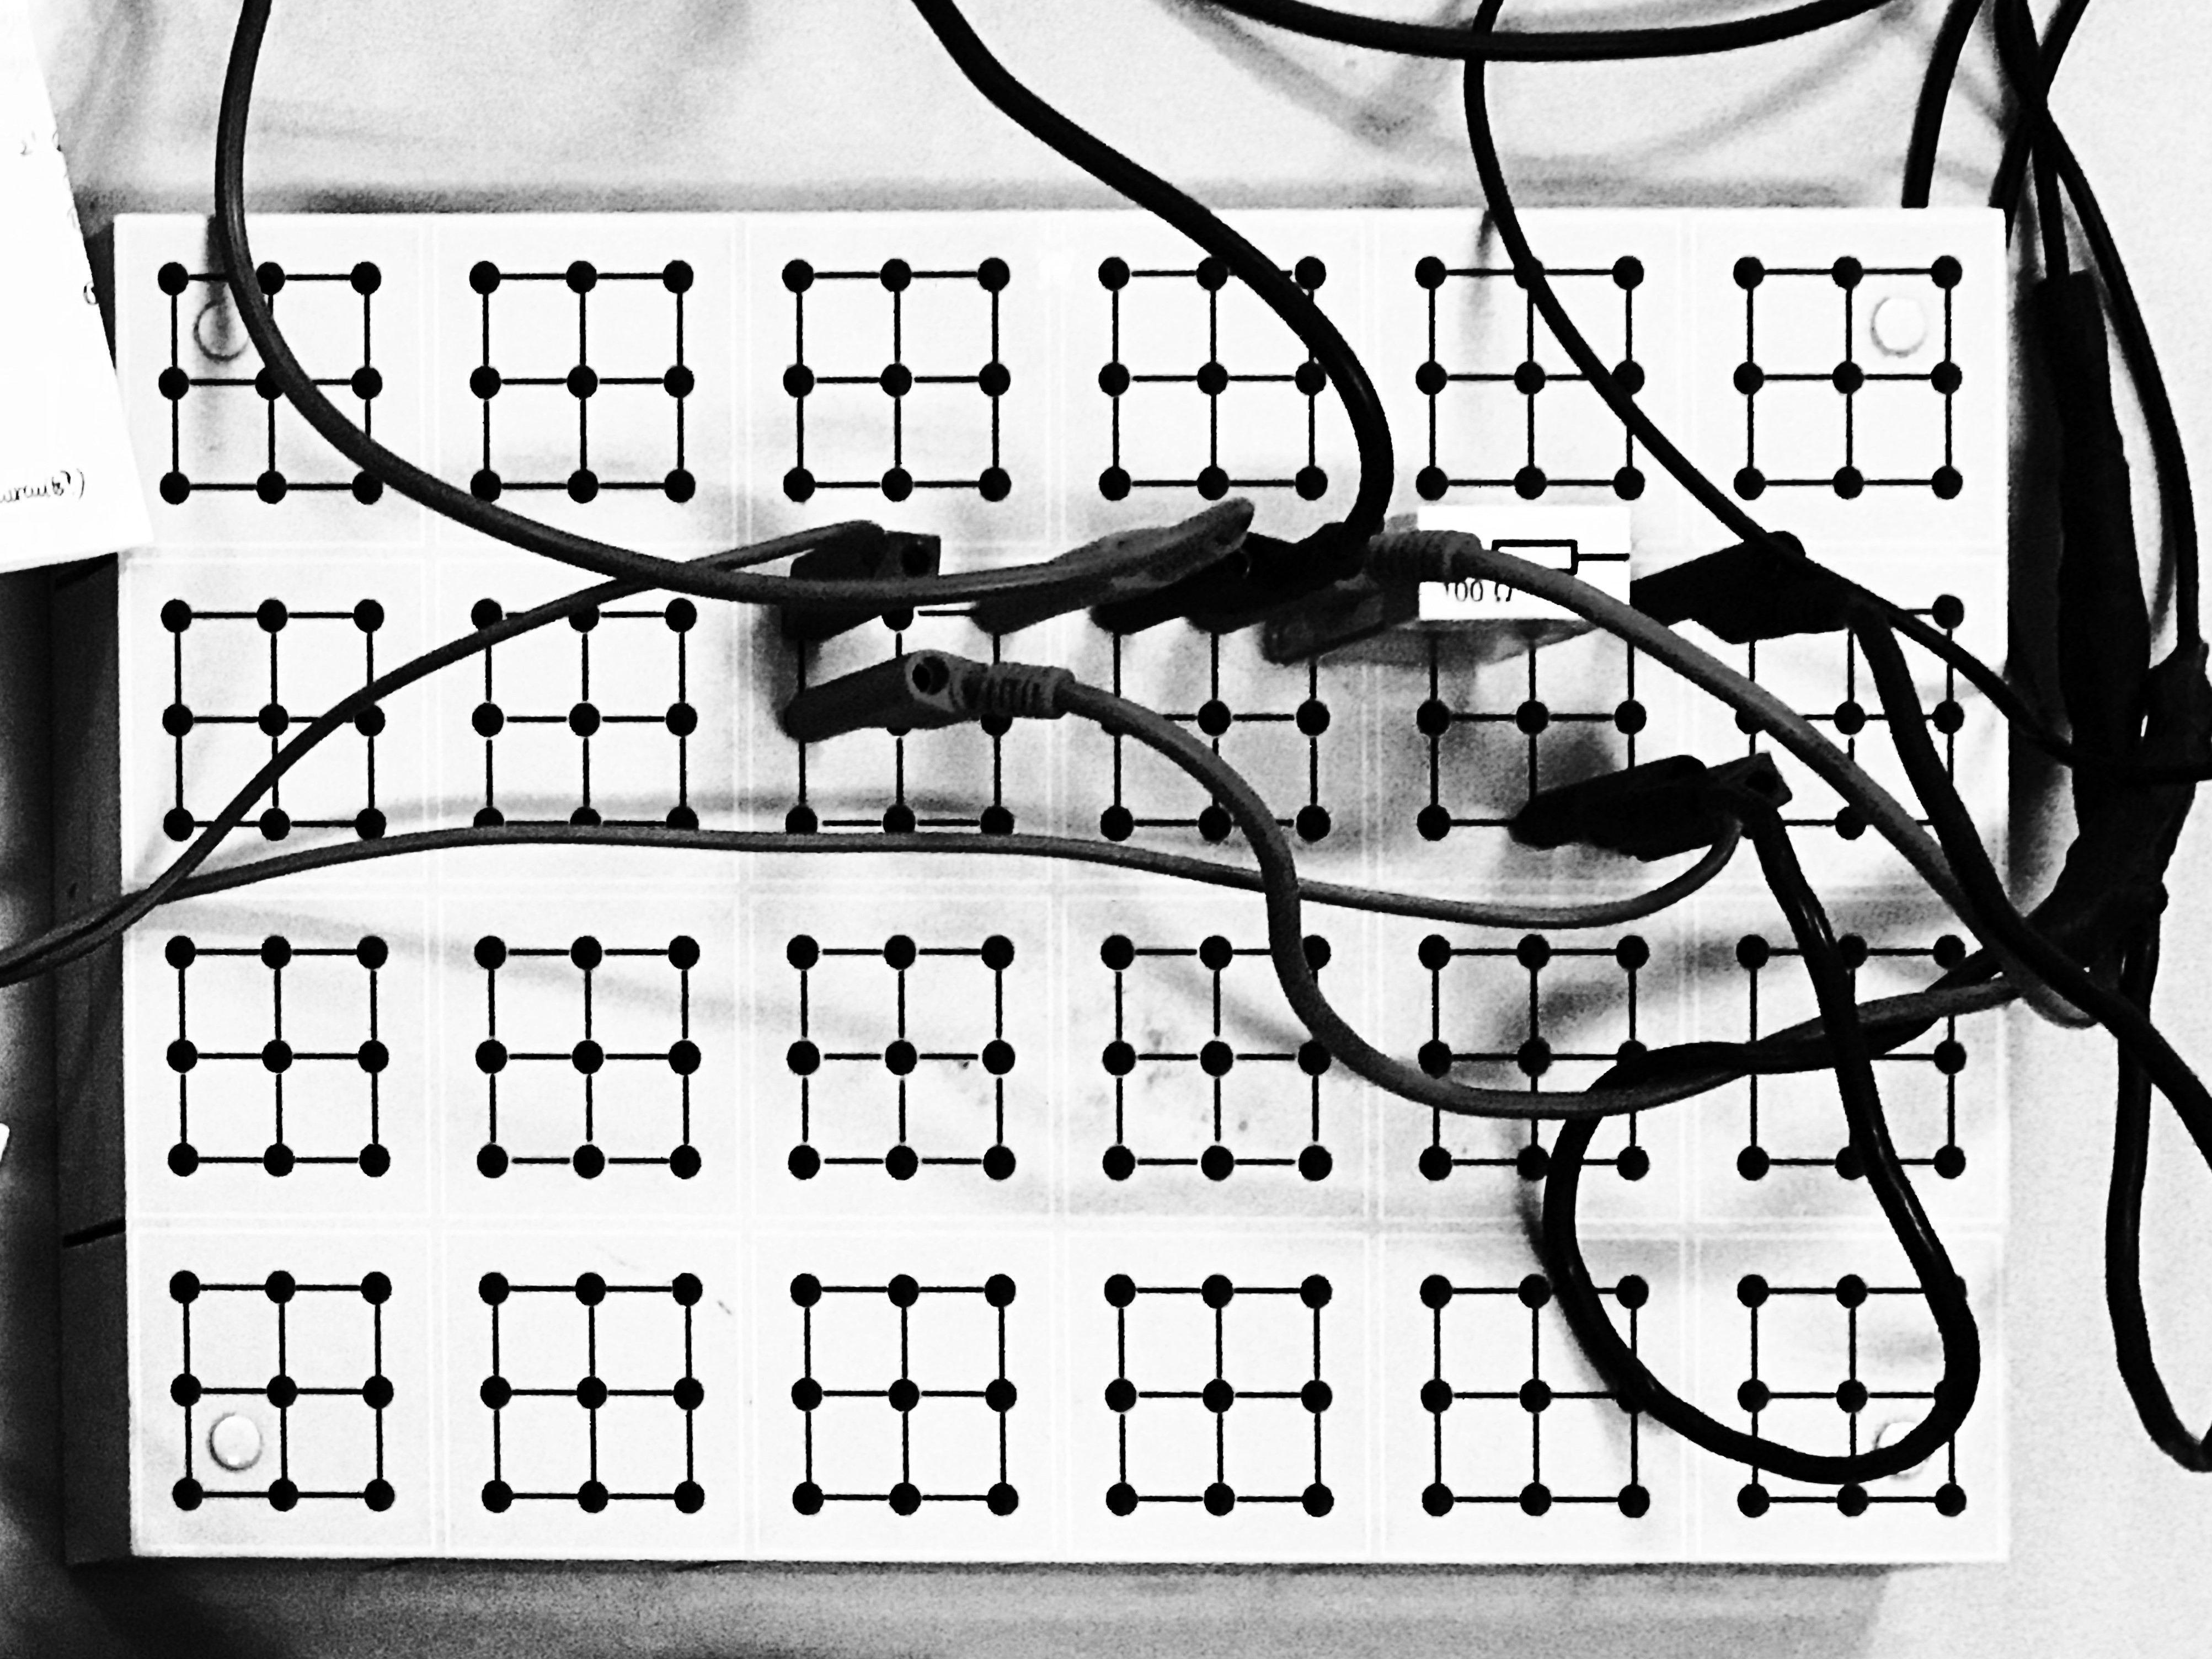
\includegraphics[width=8cm]{breadboard.jpg}
	\caption{An example of the connection of RCL circuit}
	\label{fig::breadboard}
\end{figure}

The precision of the apparatus is shown in Table \ref{table::precision}.

\begin{table}[!htbp]
	\centering
	\begin{tabular}{c c c c c}
		\hline \hline
		Apparatus                           & Measurement & Unit                     & Precision  \\
		\hline
		\multirow{2}{*}{Signal generator}   & Frequency   & [Hz]                     & 0.001      \\
		                                    & Amplitude   & [$\text{V}_{\text{pp}}$] & 0.001      \\

		\multirow{2}{*}{Oscilloscope}       & Time        & [$\mu\text{s}$]          & 0.01/0.001 \\
		                                    & Voltage     & [$\text{V}_{\text{pp}}$] & 0.01       \\

		\multirow{2}{*}{Digital multimeter} & Resistance  & [$\Omega$]               & 0.01       \\
		                                    & Capacitance & [nF]                     & 0.01       \\

		Inductor                            & Inductance  & [H]                      & 0          \\
		\hline \hline
	\end{tabular}
	\caption{Precision of the measurement instruments.}
	\label{table::precision}
\end{table}


\subsection{Measurement Procedure}

\subsubsection{RC, RL Series Circuit}

\begin{enumerate}
	\item We chose a capacitor and an inductor to assemble a circuit with the fixed-resistance 100 Ω resistor.
	\item We adjusted the output frequency of the square-wave signal provided by the signal generator and observed the change of the waveform (curve shown on the oscilloscope screen) when the time constant is smaller or greater than the half period of the square wave.
	\item We used the $\texttt{PRINT}$ function of the oscilloscope to record the waveforms.
	\item We adjust display parameters of the oscilloscope and measure $T_{1/2}$ for the studied circuits.
	\item We calculated the time constant and compare it with the theoretical value. In order to find the time constant accurately, only one period should be displayed on the oscilloscope screen.
\end{enumerate}

\subsubsection{RLC Series Circuit}

\begin{enumerate}
	\item We chose a capacitor and an inductor to assemble a RLC series circuit with the variable resistor.
	\item We observed the waveform of the capacitor voltage in the under-damped, critically damped, and over-damped regimes.
	\item We used the PRINT function of the oscilloscope to store the waveforms.
	\item We adjusted the variable resistor to the critically damped regime. According to the definition of the half-life period $ T_{1/2} $, we have $ \beta T_{1/2} = 1.68 $.
	\item We found the value of $ T_{1/2} $, and then found the time constant as $ \tau = 1/\beta = T_{1/2}/1.68 $.
	\item we compared your result with the theoretical value.
\end{enumerate}

\subsubsection{RLC Resonant Circuit}

\begin{enumerate}
	\item We applied a sinusoidal input voltage $U_i$ to the $RLC$ series circuit, and changed the frequency to observe the change of the voltage $U_R$ for a fixed resistor $R$.
	\item We observed the phase difference between $U_R$ and $U_i$.
	\item We measured how $U_R$ changes with $U_i$ and calculate the phase difference.
	\item We plotted the graphs $f/f_0$ vs. $I/I_\text{m}$ and $f/f_0$ vs. $\varphi$.
	\item We estimated the resonance frequency and calculate the quality factor $Q$.
\end{enumerate}

\subsubsection{Cations}

\begin{enumerate}
	\item The circuit should be grounded to the same point as the instruments used in the measurements. In practice, all black wires should be inserted into the same block.
	\item When measuring the corresponding element, it should be put at the side of the whole series connection. Otherwise it's hard to make sure that all black wires can be grounded.
	\item When adjusting the waves in phase, we use the feature of Lissajous' figures. The figure should present a straight line of $45^\circ$.
	\item In order to find the time constant accurately, only one period should be displayed on the oscilloscope screen.
	\item We should read manuals carefully before operating the instruments.
\end{enumerate}


\subsection{Safety Notice}

\begin{enumerate}[a.]
	\item Do not direct the laser beam into the eye.
	\item Do not touch the surface of the polarizers or the wave plates.
	\item Please leave the equipment in order before leaving.
\end{enumerate}


\section{Experimental Results}

\subsection{$T_{1/2}$ Measurement in $RC$ Series Circuit}

For $RC$ circuit, the recorded data is as follows.
\begin{table}[!htbp]
	\centering
	\begin{tabular}{ccccc}
		\hline
		R[$\Omega$]     & f[Hz]              & $\varepsilon$[Vpp] & C[nF]           & $T_{1/2}$[$\mu$s] \\
		\hline
		100.15$\pm$0.01 & 1000.000$\pm$0.001 & 4.000$\pm$0.001    & 100.57$\pm$0.01 & 9.000$\pm$0.001   \\
		\hline
	\end{tabular}%
	\caption{$T_{1/2}$ measurement data for a RC series circuit}
\end{table}

We first transform the above data into SI units for further calculations.
\begin{table}[!htbp]
	\centering
	\begin{tabular}{l c c}
		\hline
		                    & Value                  & Uncertainty        \\
		\hline
		R [$\Omega$]        & 100.15                 & 0.01               \\
		f [Hz]              & 1000.000               & 0.001              \\
		$\varepsilon$ [Vpp] & 4.000                  & 0.001              \\
		C [F]               & 1.0057$\times 10^{-7}$ & 1$\times 10^{-11}$ \\
		T$_{1/2}$ [s]       & 9.000$\times 10^{-6}$  & 1$\times 10^{-9}$  \\
		\hline
	\end{tabular}
	\caption{Transformed into SI units}
\end{table}

The experimental determined time constant $\tau$ can be calculated by

%%%%%%%%%%%%%%%%%%%

\begin{align*}
	\tau_{exp}
	 & =\frac{T_{1/2}}{\ln2}                                 \\
	 & =\frac{9.000\times 10^{-6}}{\ln2}                     \\
	 & =1.29843\times 10^{-5}\pm 1.4\times 10^{-9}[\text{s}] \\
	 & =12.9843\pm 0.0014[\mu \text{s}]
\end{align*}

Theoretically, we find that
\begin{align*}
	\tau_{theo}
	 & =RC                                                   \\
	 & =100.15\times 1.0057\times 10^{-7}                    \\
	 & =1.00721\times 10^{-5}\pm 1.4\times 10^{-9}[\text{s}] \\
	 & =10.0721\pm 0.0014[\mu \text{s}]
\end{align*}

The relative error $\delta$ can be found as

\begin{align*}
	\delta_{\tau}
	 & = \frac{\tau_{exp}-\tau_{theo}}{\tau_{theo}}\times 100\%                                \\
	 & = \frac{1.29843\times 10^{-5}-1.00721\times 10^{-5}}{1.00721\times 10^{-5}}\times 100\% \\
	 & = 28.91\%
\end{align*}

The relatively error is relatively large, thus we conclude that there might be some errors in this experiment. Hence repeated exercise is needed.
Uncertainty will be analysis in the next section and the theoretic and experimental wave graphs are plotted as follows. The theoretic graph is plotted by Origin.

\newpage
\begin{figure}[!htbp]
	\center
	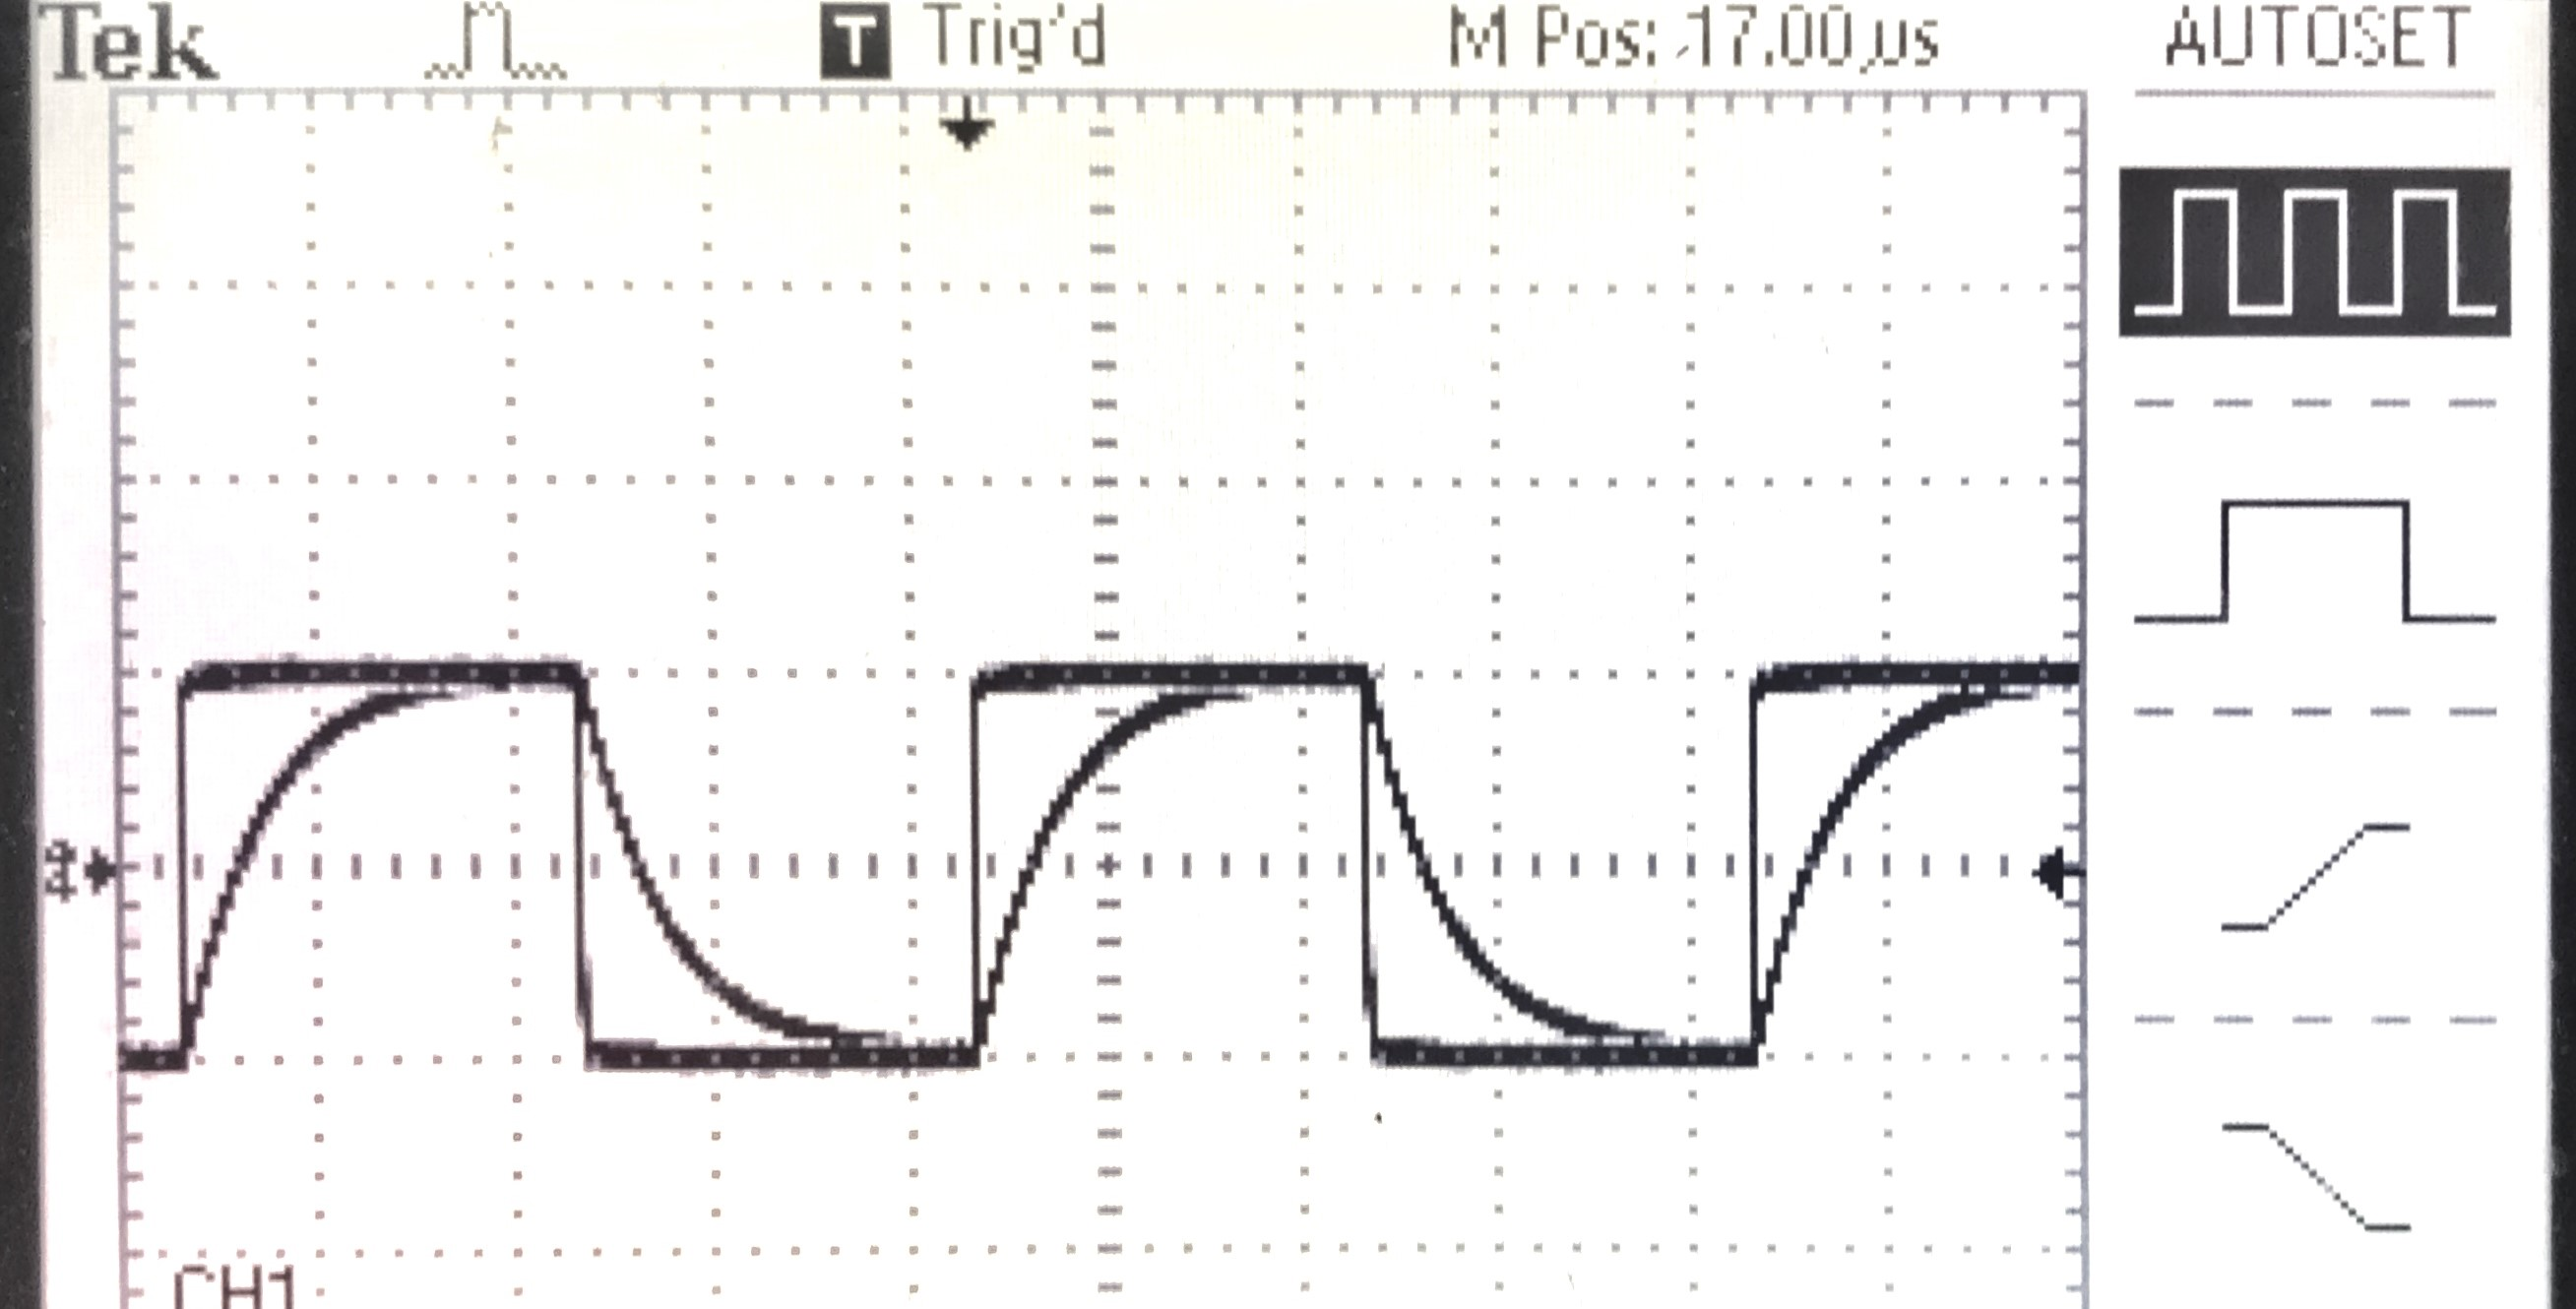
\includegraphics[width=12cm]{rc_exp.jpg}
	\caption{Experimental Results of RC circuit}
\end{figure}

\begin{figure}[!htbp]
	\center
	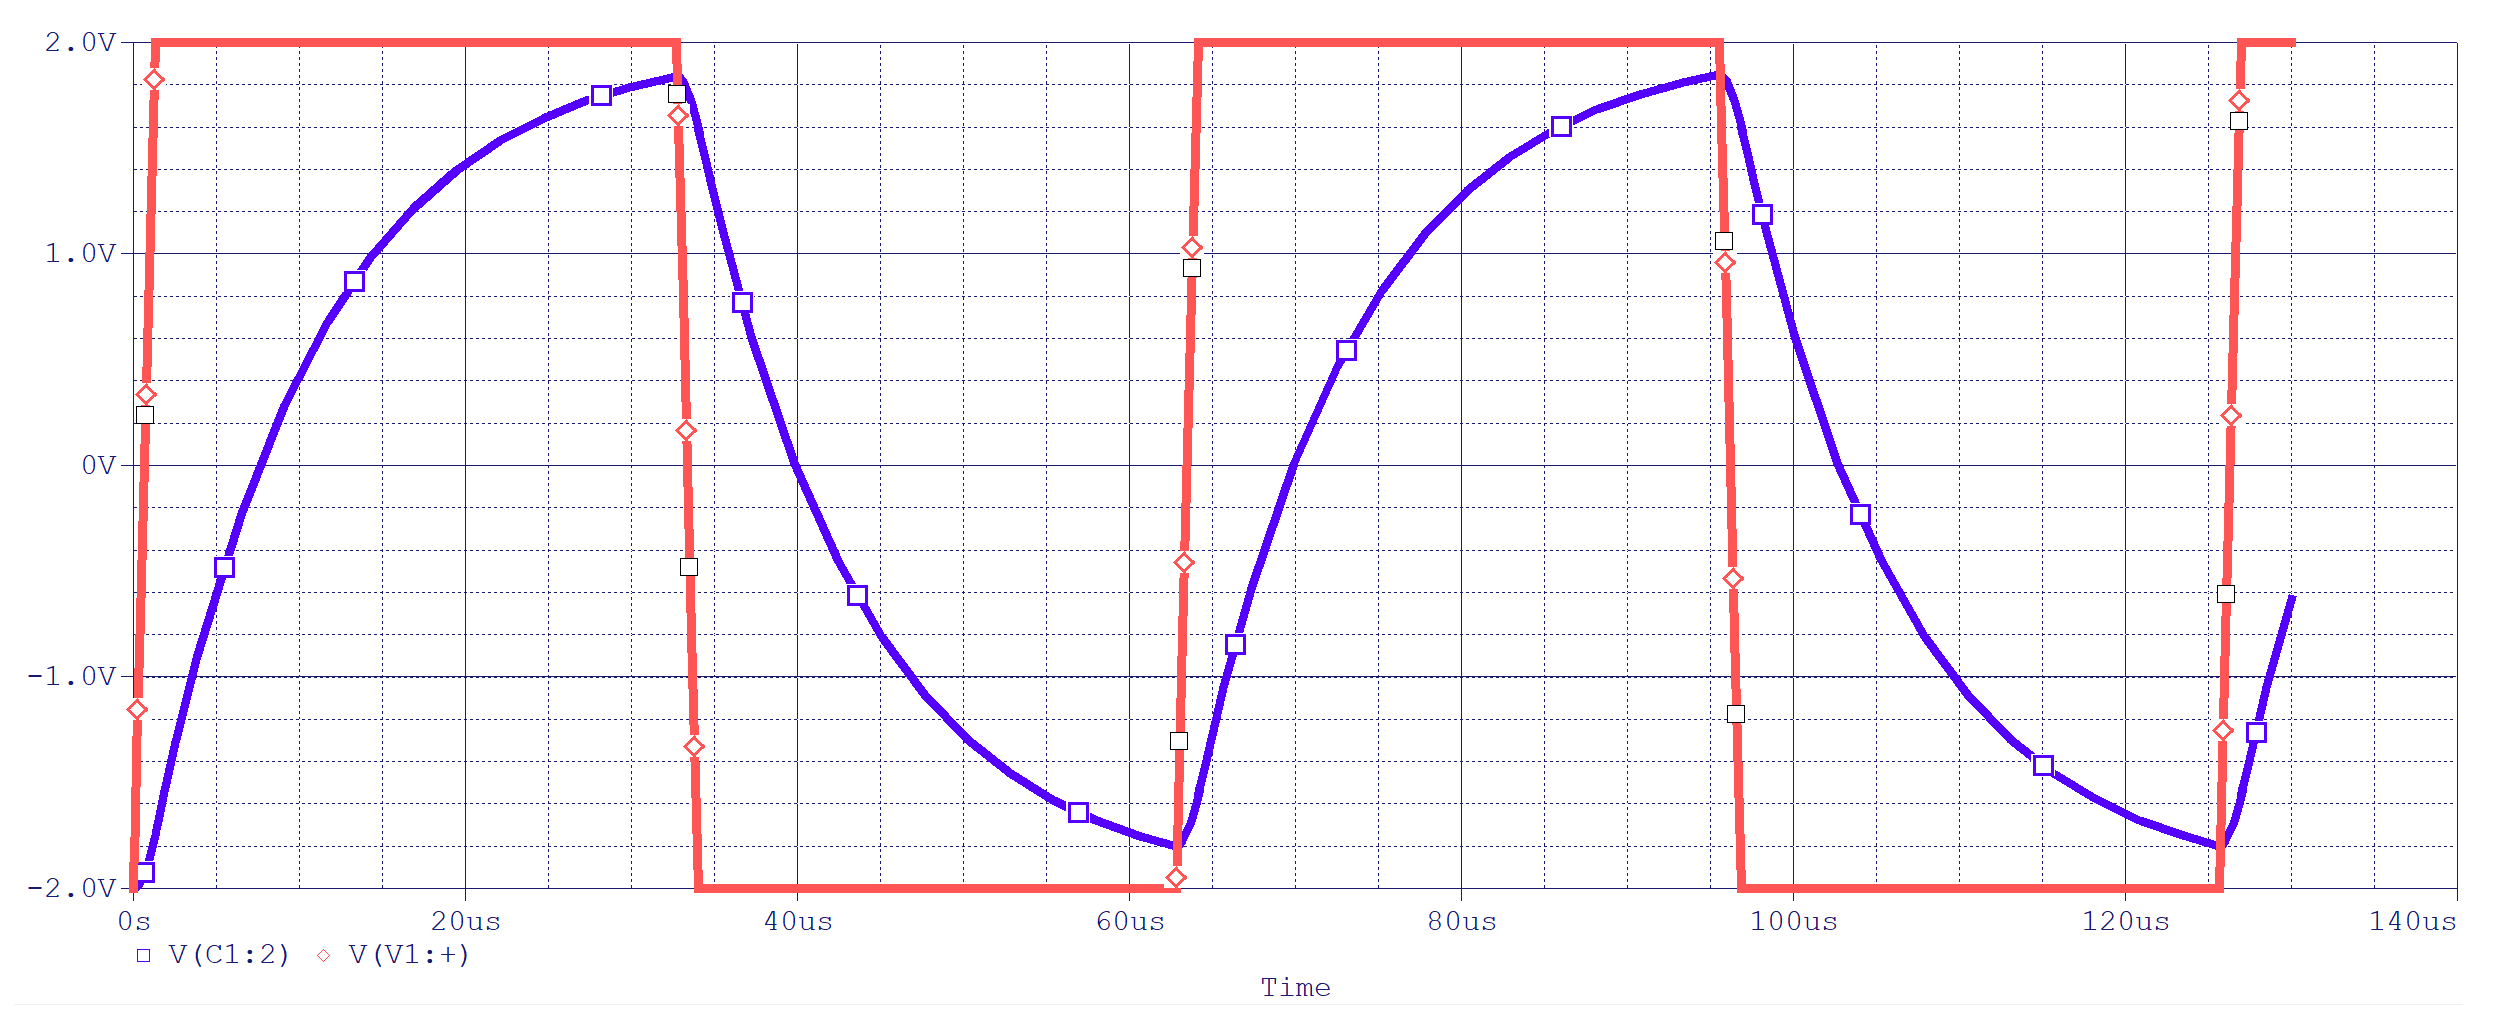
\includegraphics[width=12cm]{rc_theo.png}
	\caption{Theoretic Results of RC circuit}
\end{figure}

\subsection{$T_{1/2}$ Measurement in $RL$ Series Circuit}

For $RL$ circuit, the recorded data is as follows.
\begin{table}[!htbp]
	\centering
	\begin{tabular}{ccccc}
		\hline
		R[$\Omega$]     & f[Hz]              & $\varepsilon$[Vpp] & L[H]          & $T_{1/2}$[$\mu$s] \\
		\hline
		100.15$\pm$0.01 & 1000.000$\pm$0.001 & 4.000$\pm$0.001    & 0.01$\pm$0.01 & 80.00$\pm$0.01    \\
		\hline
	\end{tabular}%
	\caption{$T_{1/2}$ measurement data for a RL series circuit}
\end{table}

We first transform the above data into SI units for further calculations.
\begin{table}[!htbp]
	\centering
	\begin{tabular}{l c c}
		\hline
		                    & Value                 & Uncertainty       \\
		\hline
		R [$\Omega$]        & 100.15                & 0.01              \\
		f [Hz]              & 1000.000              & 0.001             \\
		$\varepsilon$ [Vpp] & 4.000                 & 0.001             \\
		L [H]               & 0.01                  & 0                 \\
		T$_{1/2}$ [s]       & 8.000$\times 10^{-5}$ & 1$\times 10^{-8}$ \\
		\hline
	\end{tabular}
	\caption{Transformed into SI units}
\end{table}

The experimental determined time constant $\tau$ can be calculated by
\begin{align*}
	\tau_{exp}
	 & =\frac{T_{1/2}}{\ln2}                                  \\
	 & =\frac{8.000\times 10^{-5}}{\ln2}                      \\
	 & =1.154156\times 10^{-4}\pm 1.4\times 10^{-9}[\text{s}] \\
	 & =115.4156\pm 0.0014[\mu \text{s}]
\end{align*}

Theoretically, we find that
\begin{align*}
	\tau_{theo}
	 & =\frac{L}{R}                                          \\
	 & =\frac{0.01}{100.15}                                  \\
	 & =9.98502\times 10^{-5}\pm 1.4\times 10^{-9}[\text{s}] \\
	 & =99.8502\pm 0.0014[\mu \text{s}]
\end{align*}

The relative error $\delta$ can be found as

\begin{align*}
	\delta_{\tau}
	 & = \frac{\tau_{exp}-\tau_{theo}}{\tau_{theo}}\times 100\%                                 \\
	 & = \frac{11.54156\times 10^{-5}-9.98502\times 10^{-5}}{9.98502\times 10^{-5}}\times 100\% \\
	 & = 15.59\%
\end{align*}

The relatively error is relatively large, thus we conclude that potential repeated experiments are needed.
Uncertainty will be analysis in the next section and the theoretic and experimental wave graphs are plotted as follows. The theoretic graph is plotted by Origin.


\begin{figure}[H]
	\center
	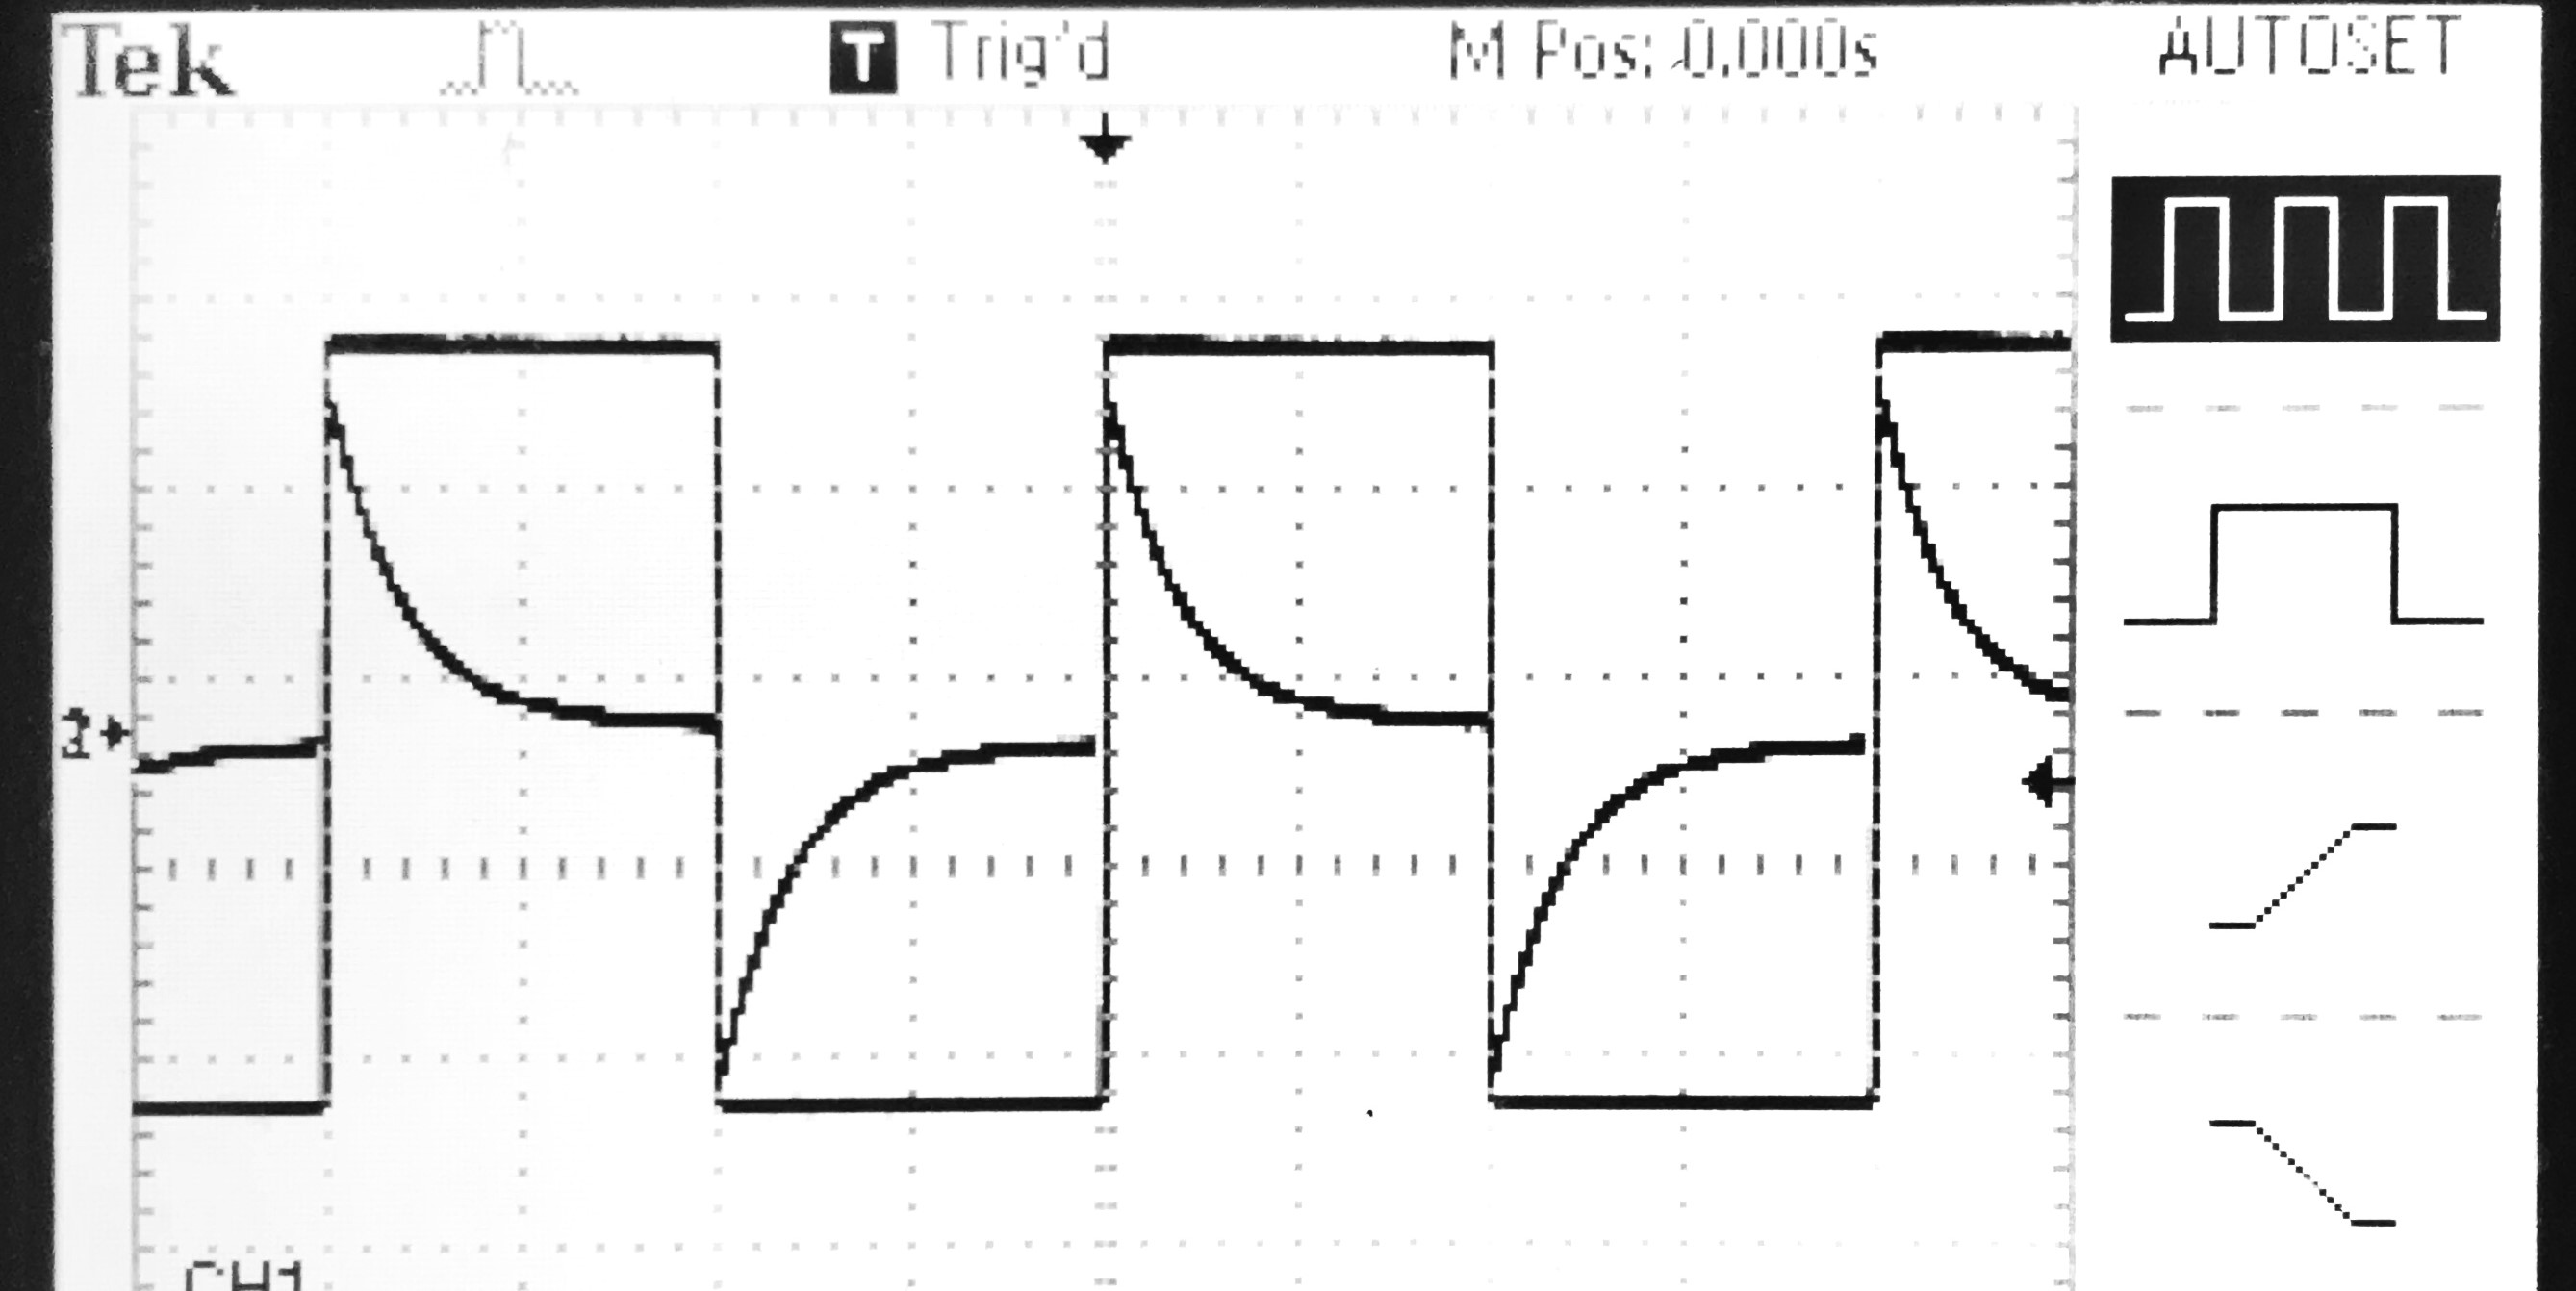
\includegraphics[width=12cm]{rl_exp.jpg}
	\caption{Experimental Results of RL circuit}
\end{figure}

\begin{figure}[H]
	\center
	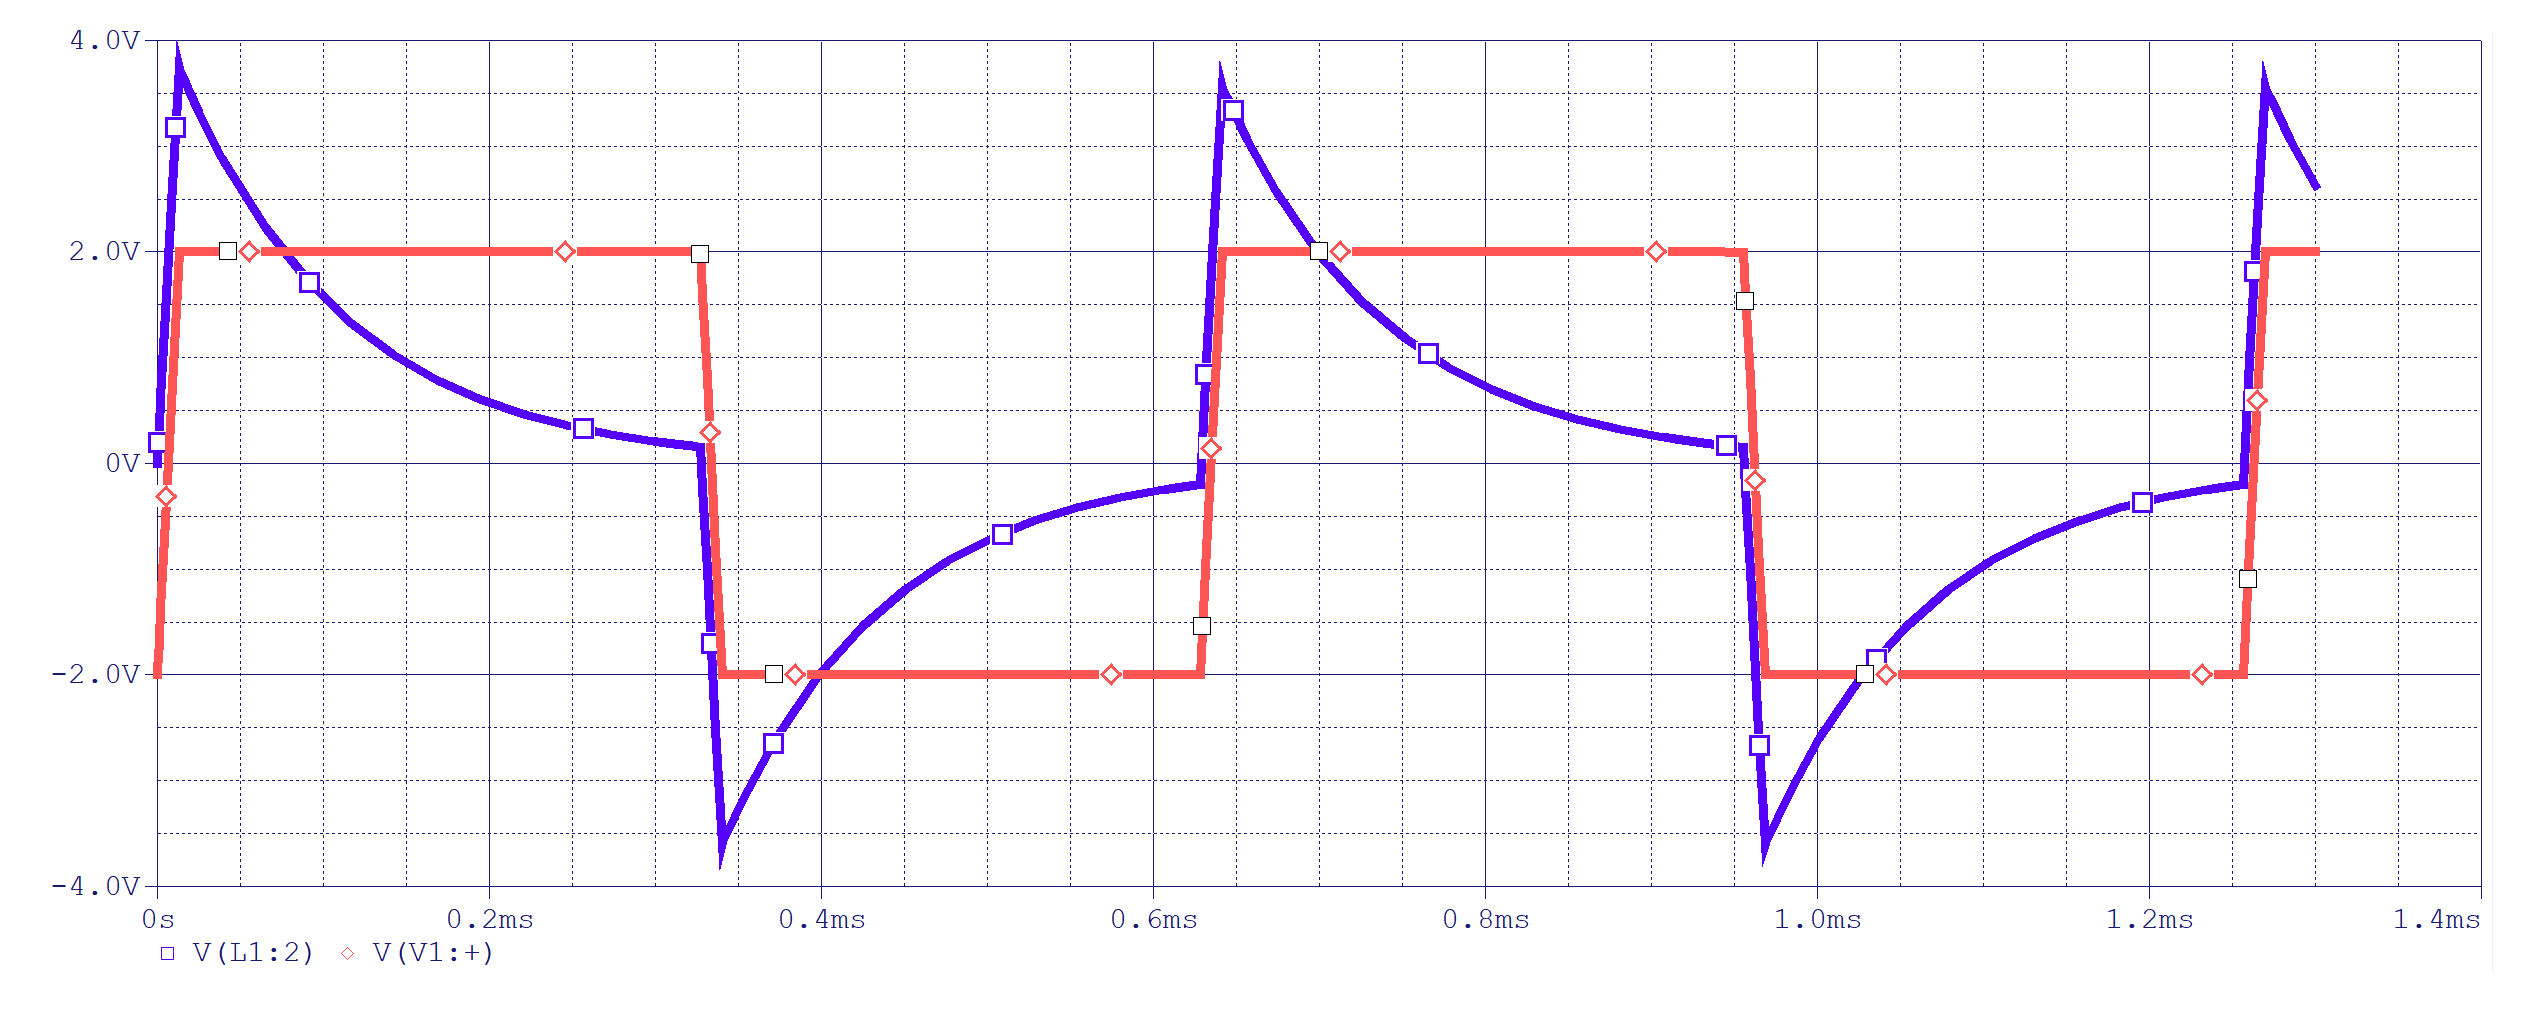
\includegraphics[width=12cm]{rl_theo.png}
	\caption{Theoretic Results of RL circuit}
\end{figure}


\subsection{$T_{1/2}$ Measurement in $RLC$ Series Circuit}

In this section, we first sow the 3 possible regimes of the $RLC$ circuit by adjusting the variable resistance. The 3 kinds of regimes are under-, over- and critically damped.
The following is a display of all wave presentation of the regimes.

The following is the under-damped situation.

\begin{figure}[H]
	\center
	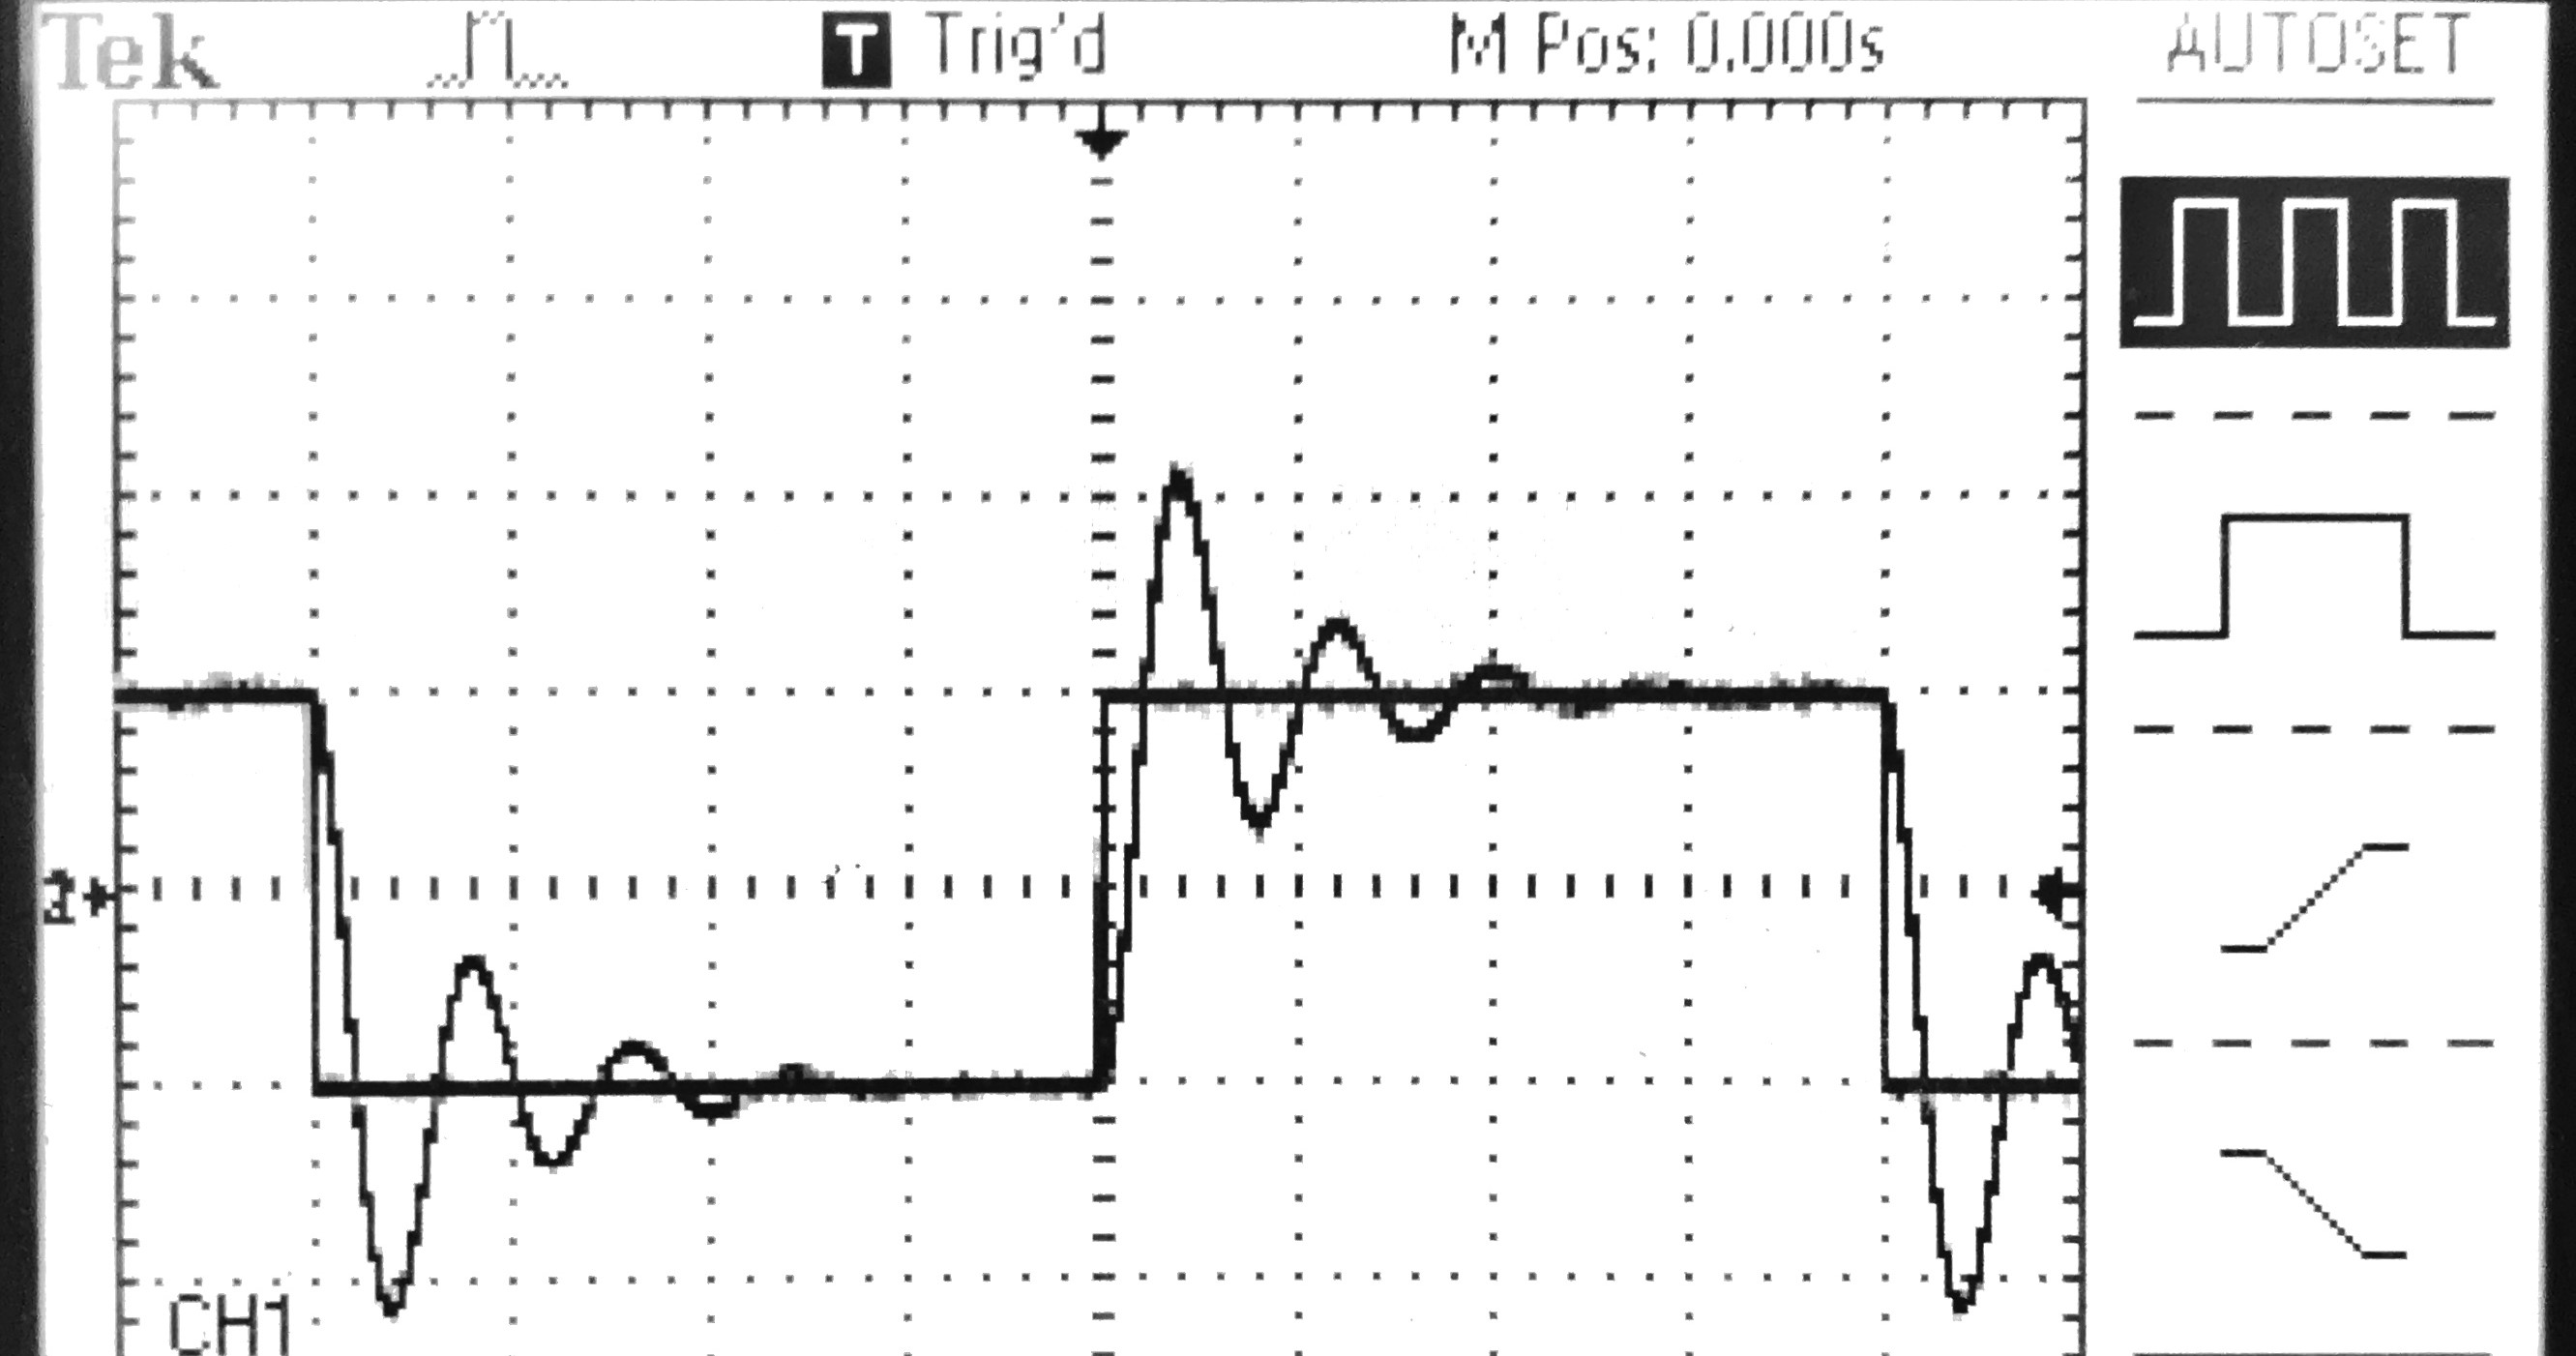
\includegraphics[width=12cm]{under_exp.jpg}
	\caption{Experimental Results of under-damped RCL circuit}
\end{figure}

\begin{figure}[H]
	\center
	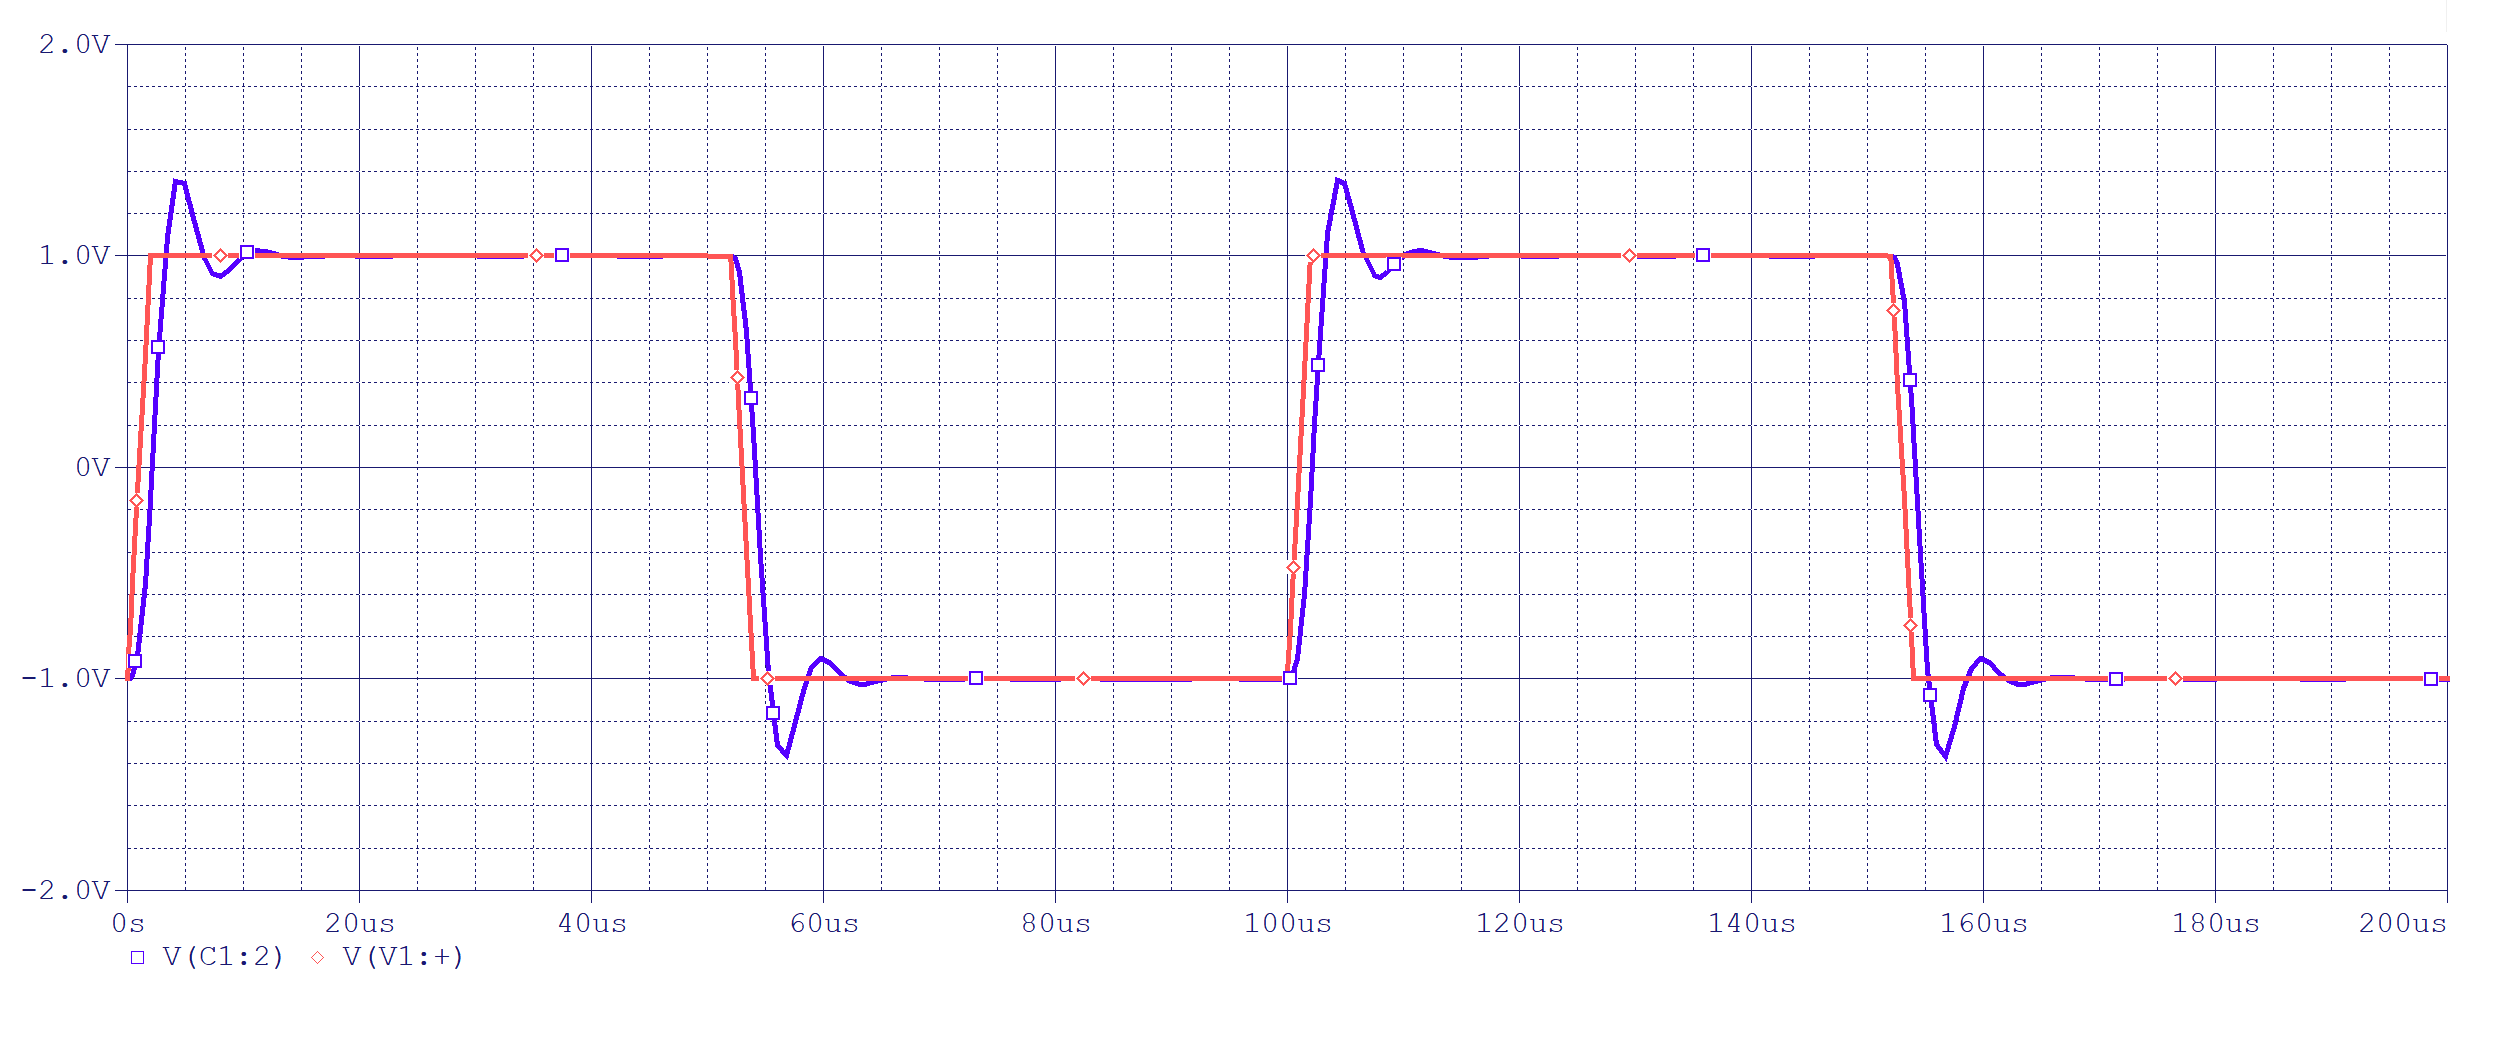
\includegraphics[width=12cm]{under_theo.png}
	\caption{Theoretic Results of under-damped RCL circuit}
\end{figure}


The following is the over-damped situation.

\begin{figure}[H]
	\center
	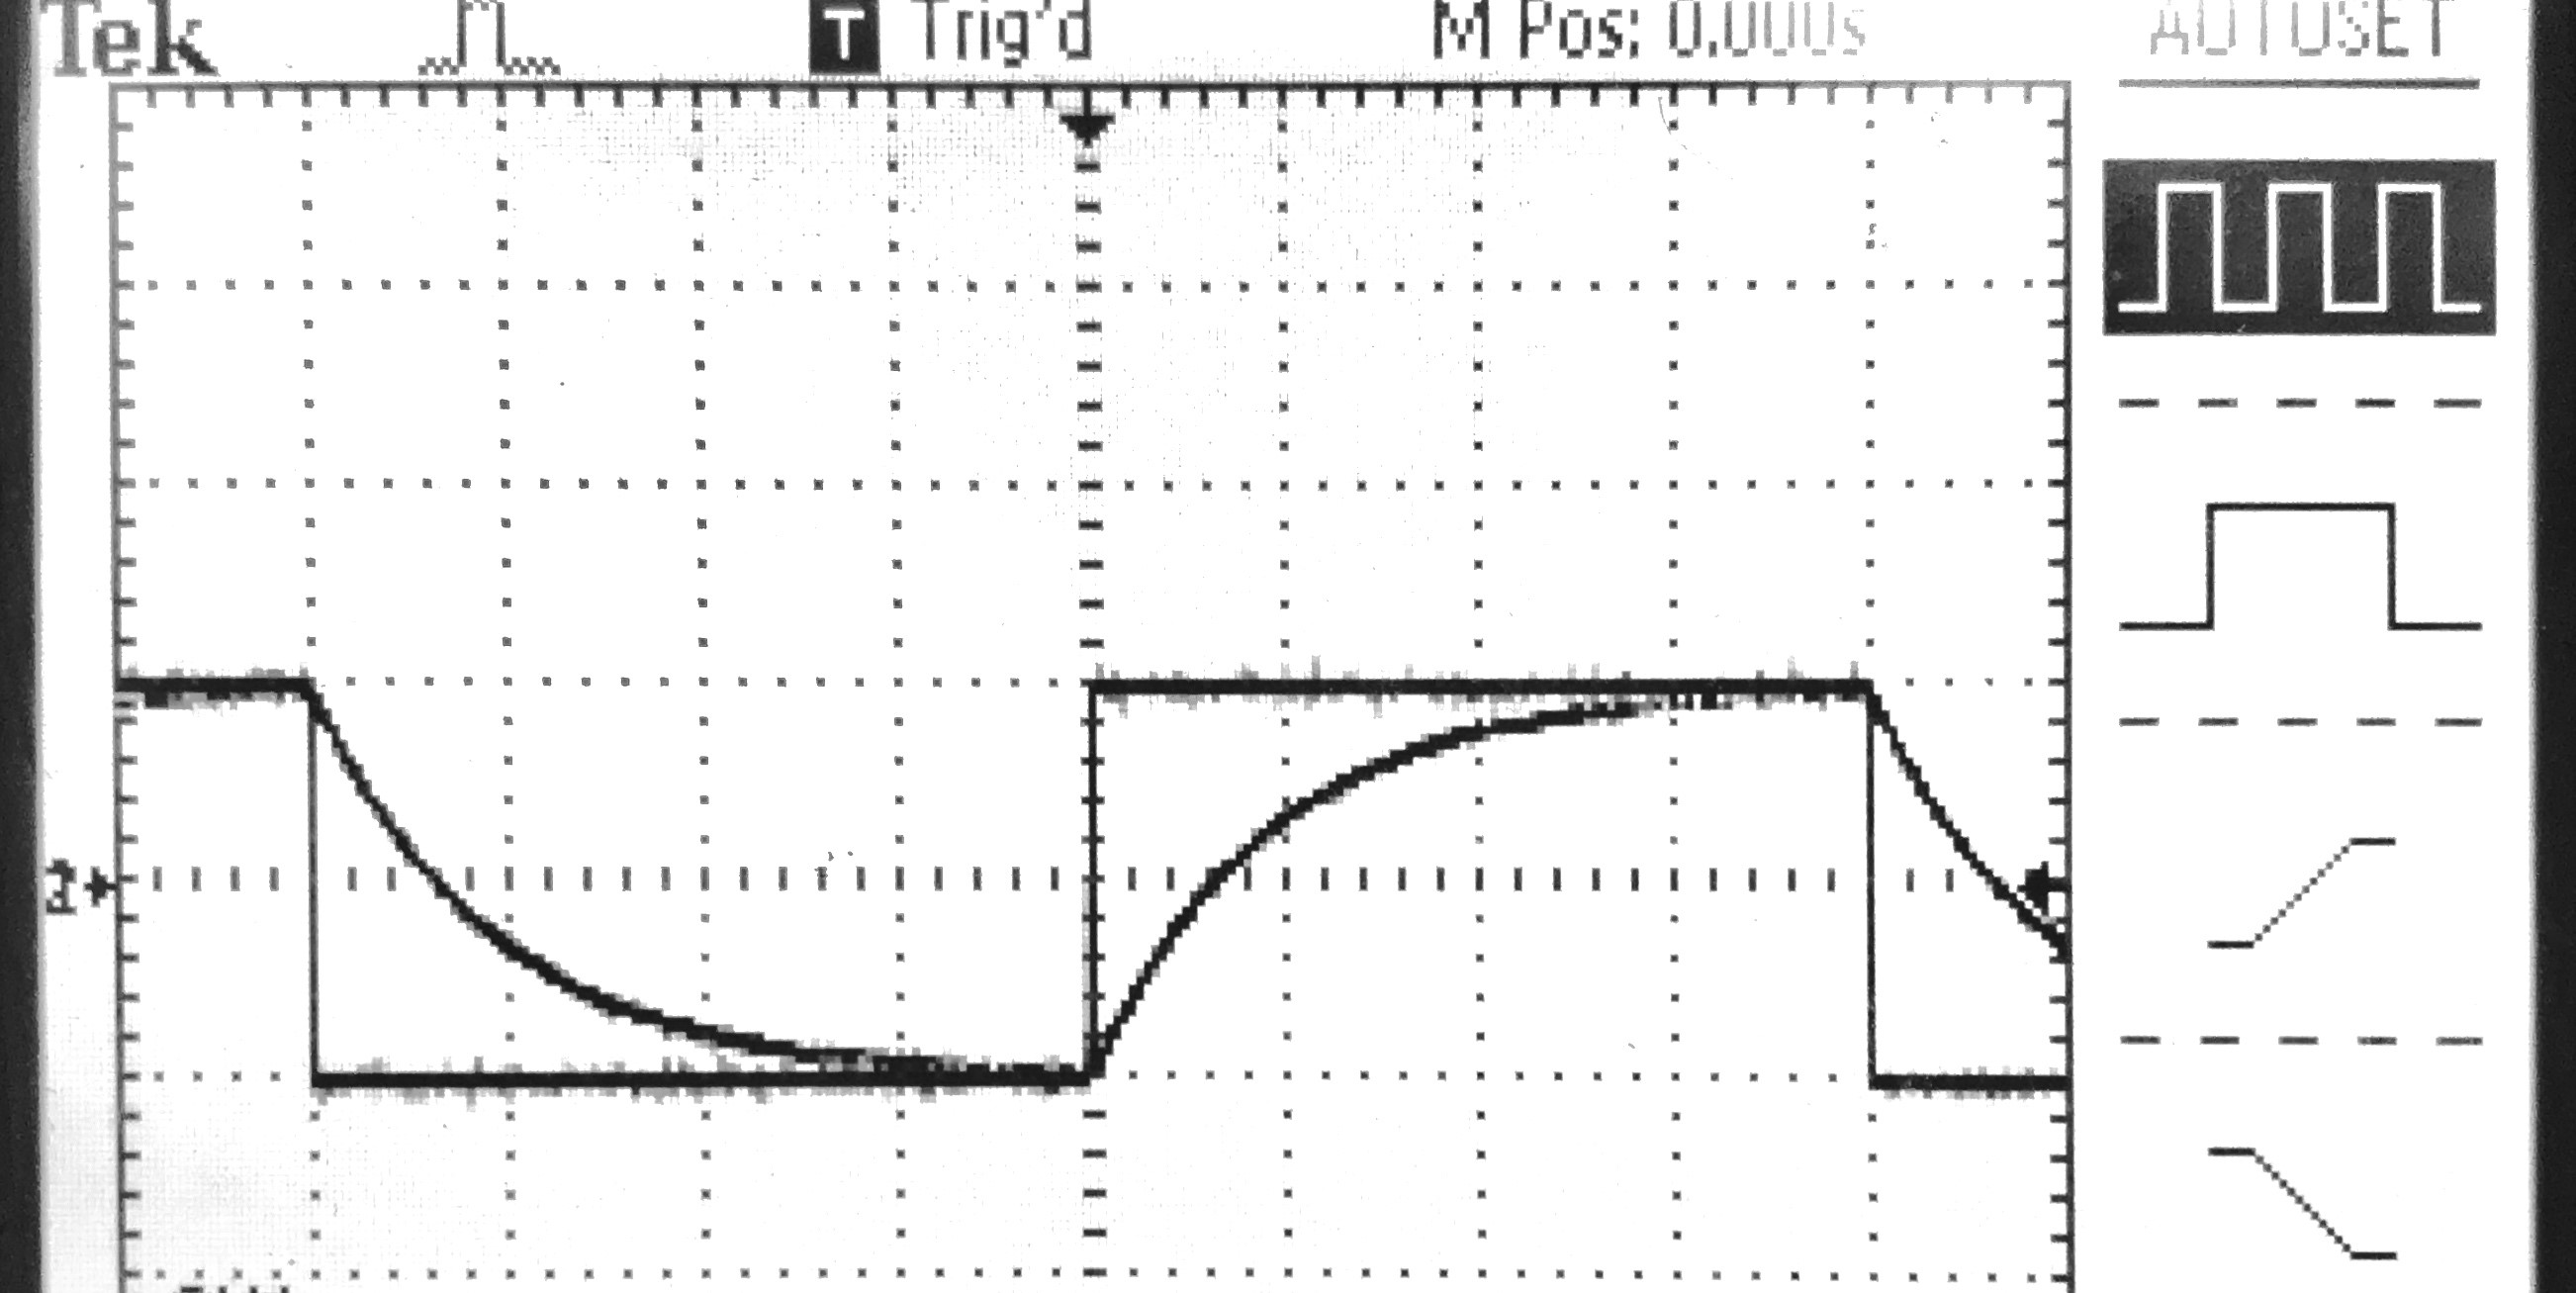
\includegraphics[width=12cm]{over_exp.jpg}
	\caption{Experimental Results of over-damped RCL circuit}
\end{figure}

\begin{figure}[H]
	\center
	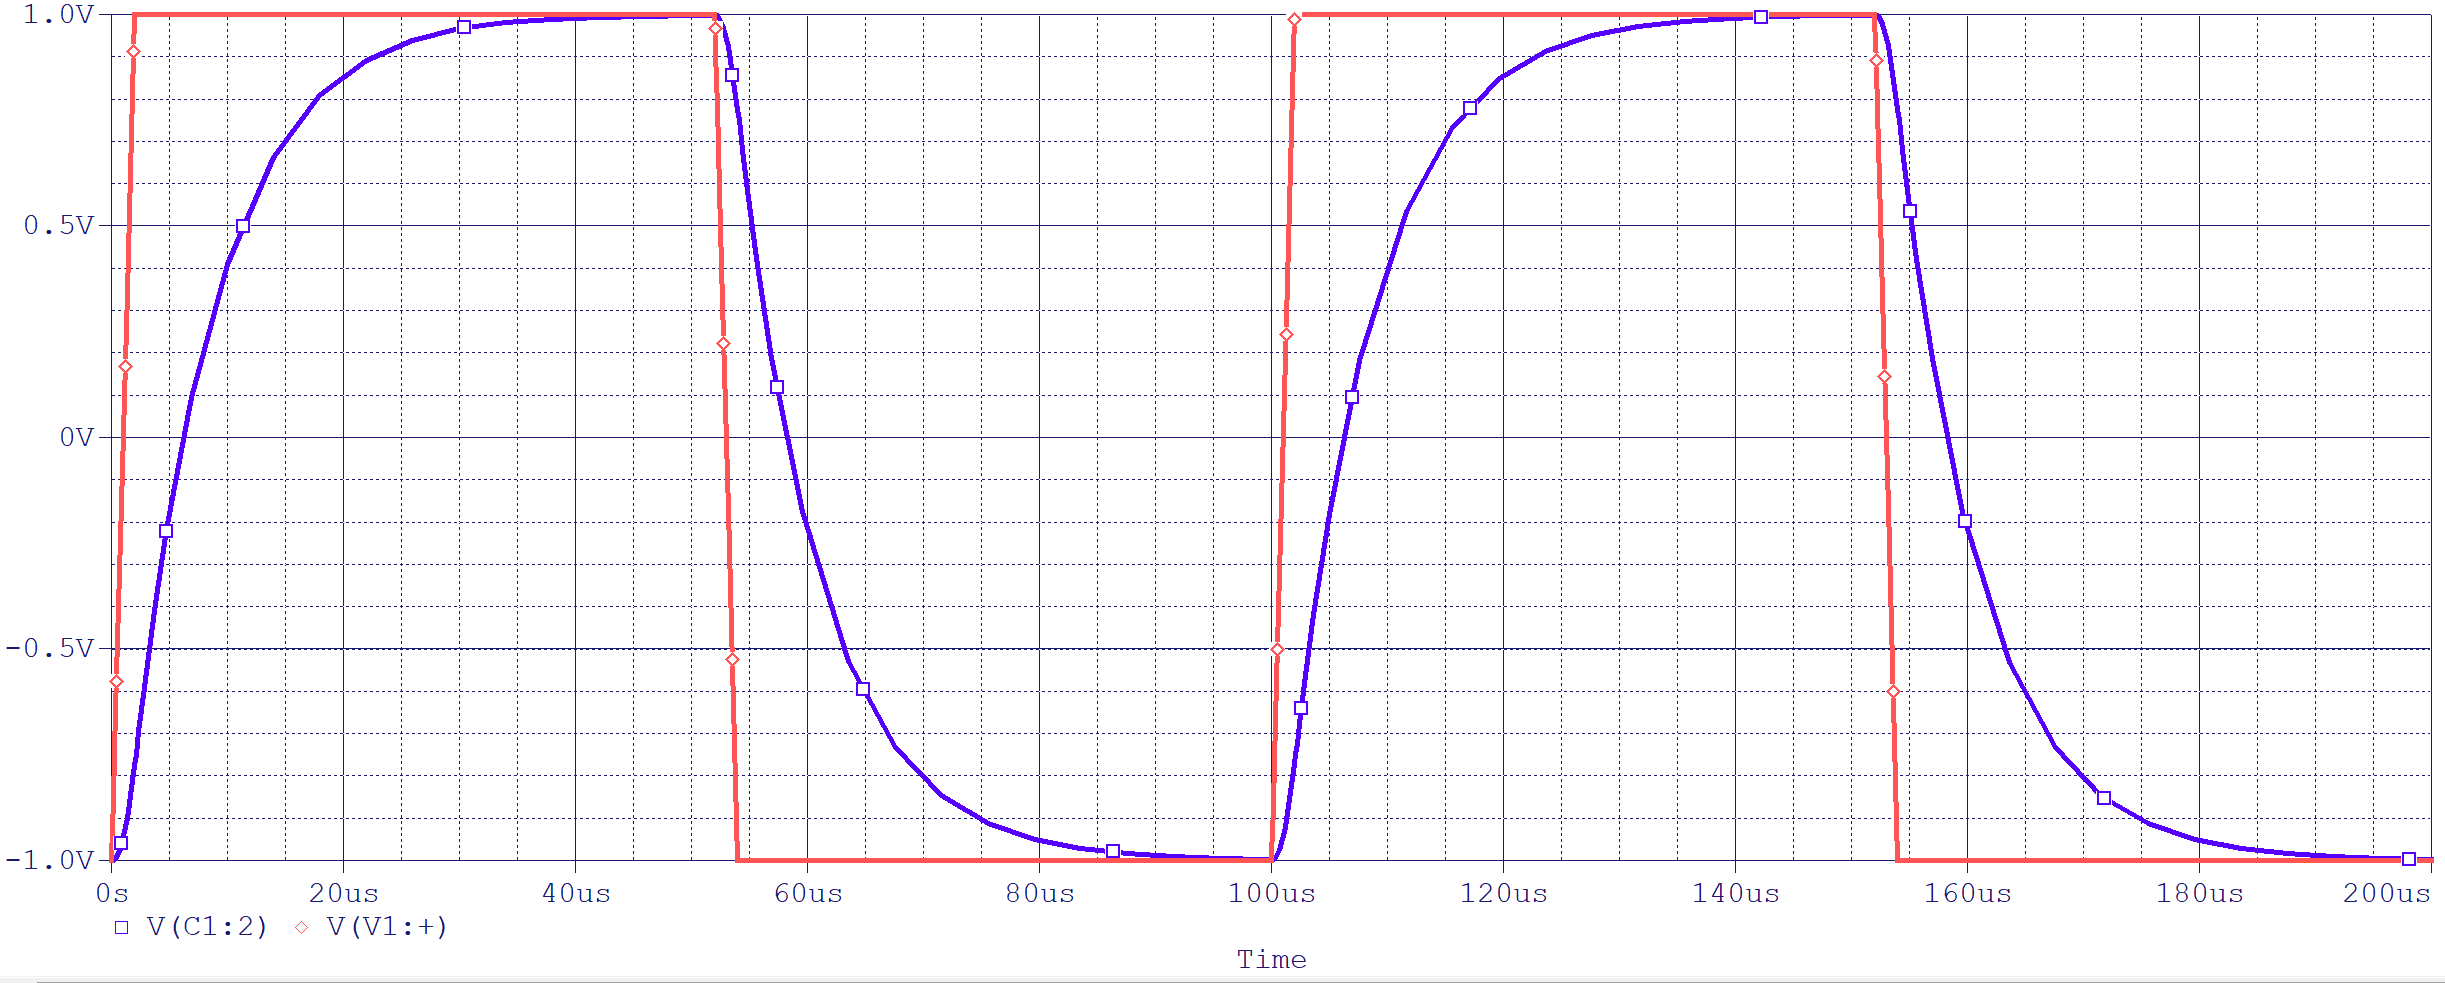
\includegraphics[width=12cm]{over_theo.png}
	\caption{Theoretic Results of over-damped RCL circuit}
\end{figure}


The following is the critically damped situation.

\begin{figure}[H]
	\center
	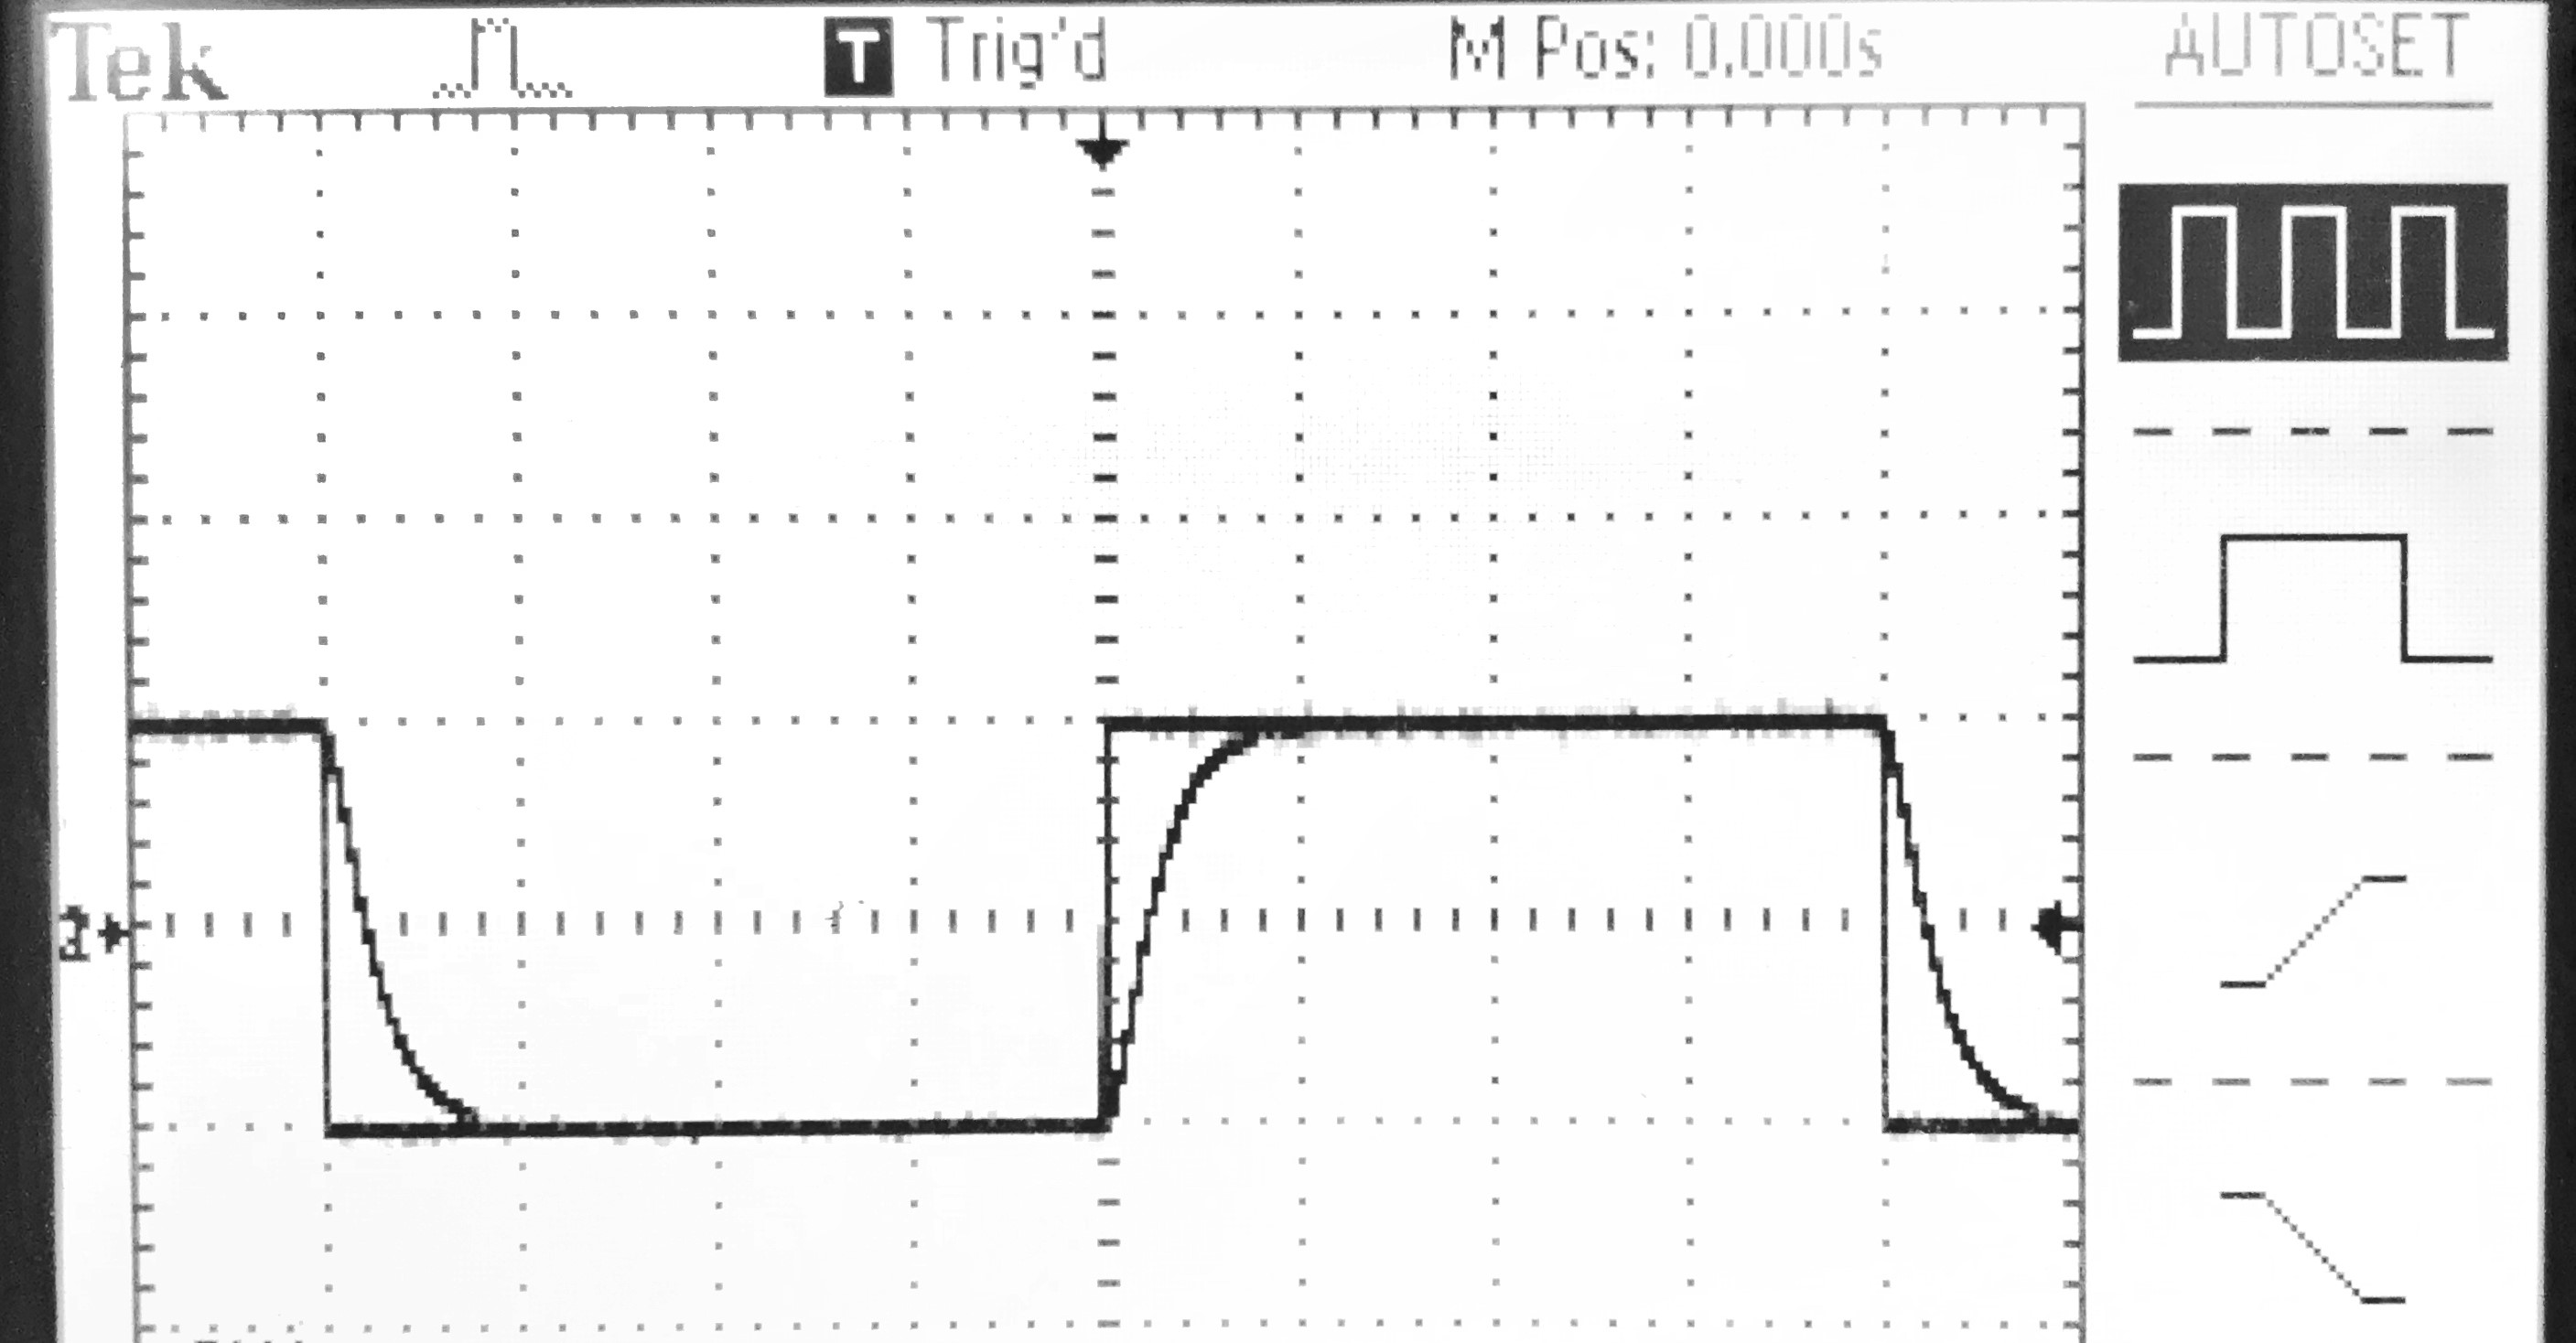
\includegraphics[width=12cm]{critical_exp.jpg}
	\caption{Experimental Results of critically damped RCL circuit}
\end{figure}

\begin{figure}[H]
	\center
	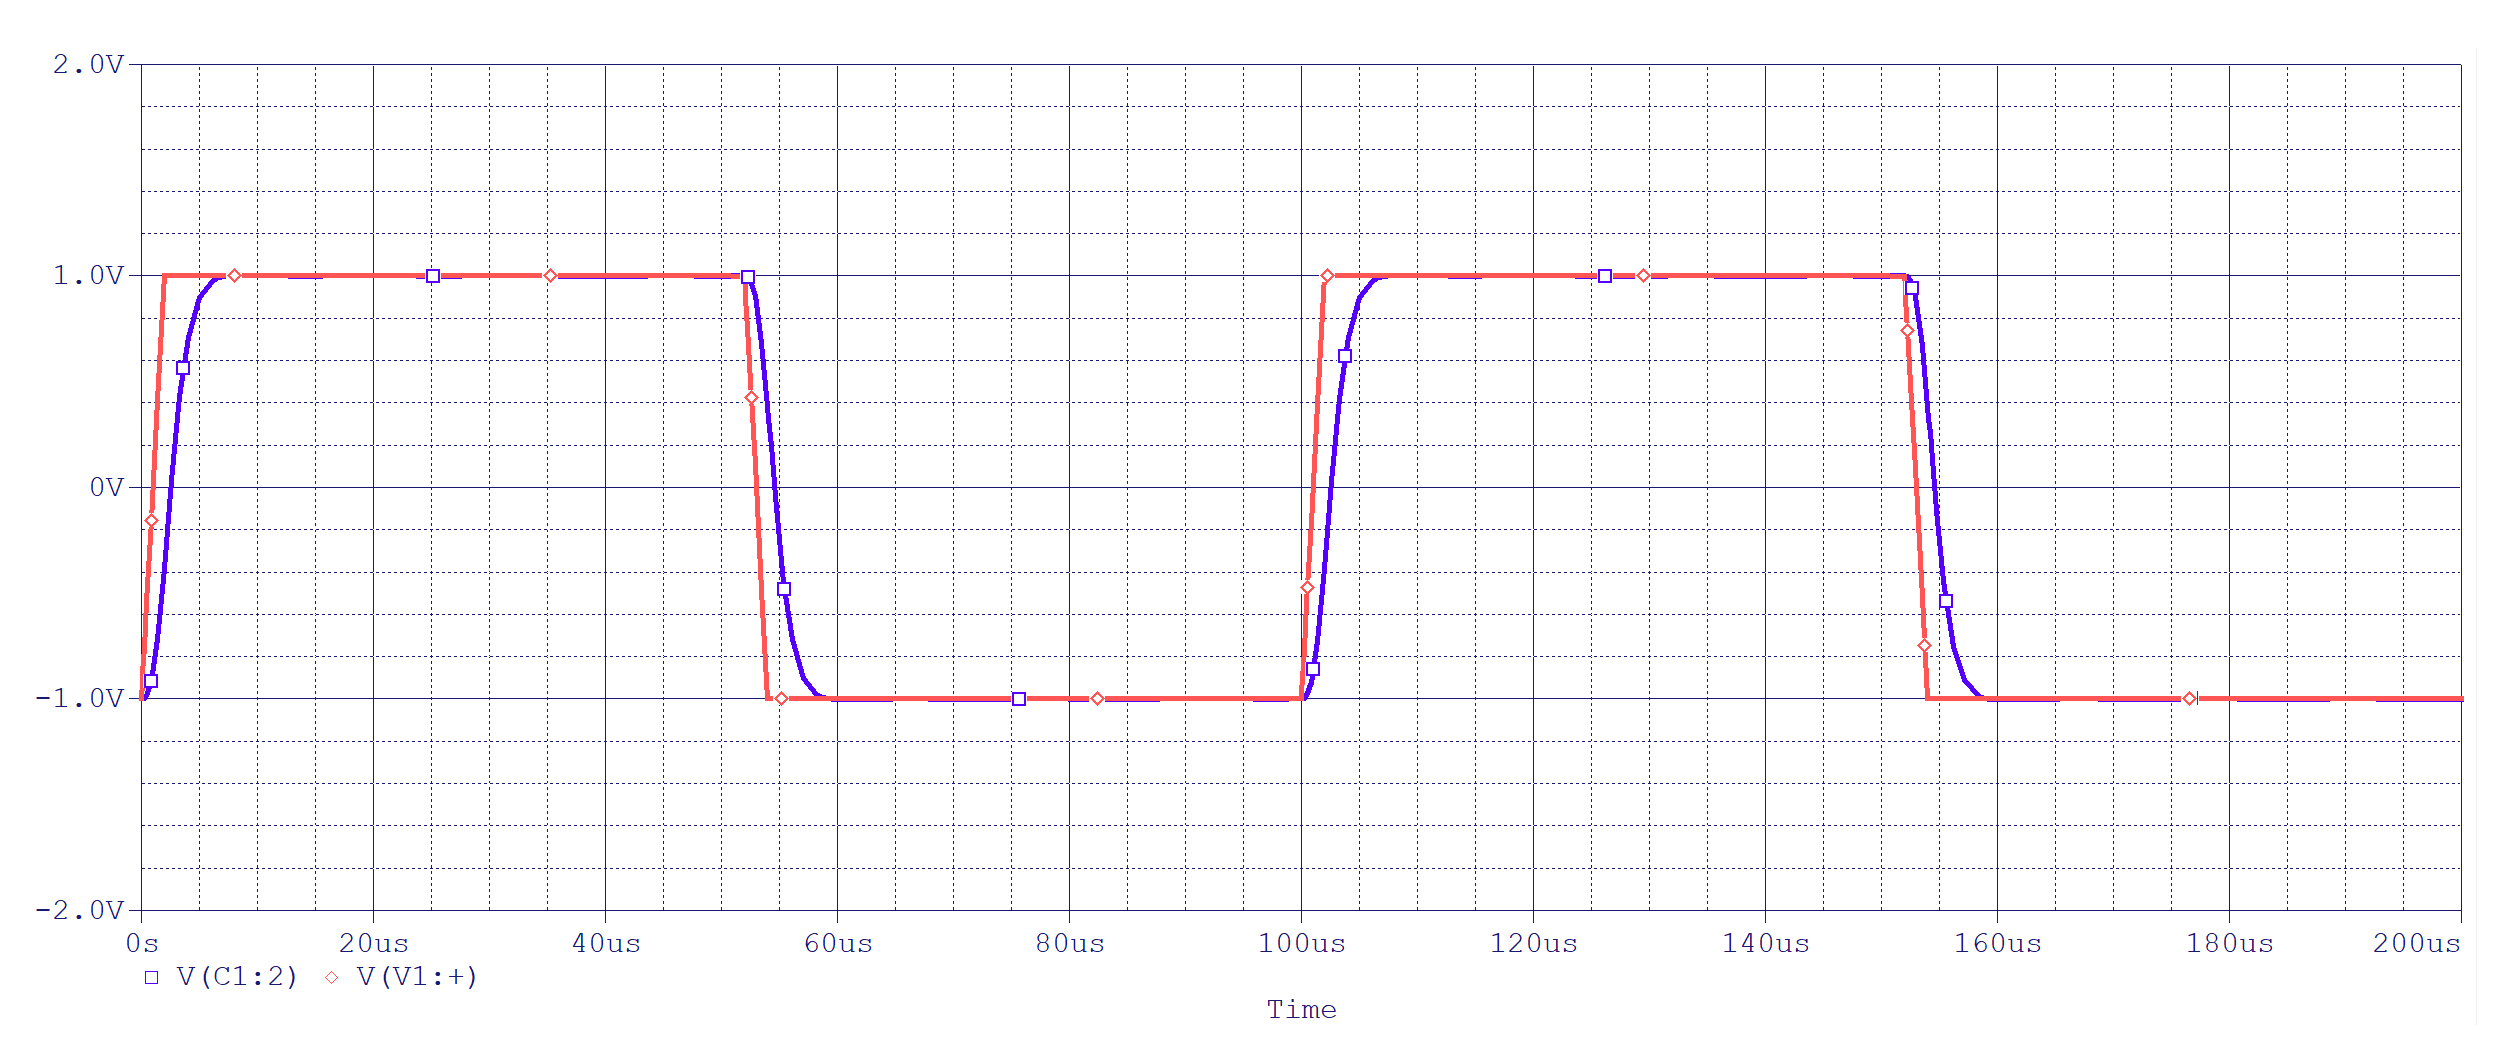
\includegraphics[width=12cm]{critical_theo.png}
	\caption{Theoretic Results of critically damped RCL circuit}
\end{figure}


We conducted $T_{1/2}$ measurement data to critically damped RLC series circuit. the recorded data is as follows.

\begin{table}[htbp]
	\centering
	\begin{tabular}{cccccc}
		\hline
		L[H]       & C[nF]           & f[Hz]              & $\varepsilon$ [Vpp] & $\beta t[s]$ & $T_{1/2}$[$\mu$s] \\
		\hline
		0.01$\pm$0 & $100.57\pm$0.01 & 1000.000$\pm$0.001 & 4.000$\pm$0.001     & 1.68         & 30.00$\pm$0.01    \\
		\hline
	\end{tabular}%
	\caption{$T_{1/2}$ measurement data for a RL series circuit}
\end{table}
where $\beta t$ is calculated as 1.68 (Measurement Procedure Part).

We first transform the above data into SI units for further calculations.
\begin{table}[!htbp]
	\centering
	\begin{tabular}{l c c}
		\hline
		                    & Value                  & Uncertainty        \\
		\hline
		f [Hz]              & 1000.000               & 0.001              \\
		$\varepsilon$ [Vpp] & 4.000                  & 0.001              \\
		C [F]               & 1.0057$\times 10^{-7}$ & 1$\times 10^{-11}$ \\
		L [H]               & 0.01                   & 0                  \\
		T$_{1/2}$ [s]       & 3.000$\times 10^{-5}$  & 1$\times 10^{-8}$  \\
		\hline
	\end{tabular}
	\caption{Transformed into SI units}
\end{table}

The experimental determined time constant $\tau$ can be calculated by
\begin{align*}
	\tau_{exp}
	 & =\frac{T_{1/2}}{\beta t}                             \\
	 & =\frac{3.000\times 10^{-5}}{1.68}                    \\
	 & =1.7857\times 10^{-5}\pm 1.4\times 10^{-8}[\text{s}] \\
	 & =17.857\pm 0.014[\mu \text{s}]
\end{align*}

Theoretically, we find that
\begin{align*}
	\tau_{theo}
	 & =\sqrt{LC}                                           \\
	 & =\sqrt{0.01\times 1.0057\times 10^{-7}}              \\
	 & =3.1713\times 10^{-5}\pm 1.0\times 10^{-8}[\text{s}] \\
	 & =31.713\pm 0.010[\mu \text{s}]
\end{align*}

The relative error $\delta$ can be found as

\begin{align*}
	\delta_{\tau}
	 & = \frac{\tau_{exp}-\tau_{theo}}{\tau_{theo}}\times 100\%                             \\
	 & = \frac{1.7857\times 10^{-5}-3.1713\times 10^{-5}}{3.1713\times 10^{-5}}\times 100\% \\
	 & = -43.69\%
\end{align*}

\subsection{Measurements for $RLC$ Resonance Circuit}

For $RLC$ circuit, the recorded condition data is as follows.
\begin{table}[!htbp]
	\centering
	\begin{tabular}{ccccc}
		\hline
		R[$\Omega$]     & L[H]       & C[nF]           & $f_0$[Hz]          & $\varepsilon$[Vpp] \\
		\hline
		100.15$\pm$0.01 & 0.01$\pm$0 & 100.57$\pm$0.01 & 5000.000$\pm$0.001 & 4.000$\pm$0.001    \\
		\hline
	\end{tabular}%
	\caption{Measurement data for a $RLC$ resonance circuit}
\end{table}

Measurement data for the $U_R$ vs. $f$ dependence for a RLC resonant circuit are presented in the following table.

\begin{table}[!htbp]
	\centering
	\begin{tabular}{c|cc|cc}
		\hline
		   & $U_R$ [Vpp] & $u_u$ [Vpp] & $f$ [Hz] & $u_f$ [Hz] \\
		\hline
		1  & 0.520       & 0.001       & 1500.000 & 0.001      \\
		2  & 0.720       & 0.001       & 2000.000 & 0.001      \\
		3  & 0.960       & 0.001       & 2500.000 & 0.001      \\
		4  & 1.28        & 0.01        & 3000.000 & 0.001      \\
		5  & 1.68        & 0.01        & 3500.000 & 0.001      \\
		6  & 2.40        & 0.01        & 4000.000 & 0.001      \\
		7  & 2.68        & 0.01        & 4200.000 & 0.001      \\
		8  & 3.08        & 0.01        & 4400.000 & 0.001      \\
		9  & 3.44        & 0.01        & 4600.000 & 0.001      \\
		10 & 3.72        & 0.01        & 4800.000 & 0.001      \\
		11 & 3.84        & 0.01        & 5000.000 & 0.001      \\
		12 & 3.76        & 0.01        & 5200.000 & 0.001      \\
		13 & 3.56        & 0.01        & 5400.000 & 0.001      \\
		14 & 3.24        & 0.01        & 5600.000 & 0.001      \\
		15 & 2.96        & 0.01        & 5800.000 & 0.001      \\
		16 & 2.64        & 0.01        & 6000.000 & 0.001      \\
		17 & 2.12        & 0.01        & 6500.000 & 0.001      \\
		18 & 1.72        & 0.01        & 7000.000 & 0.001      \\
		19 & 1.48        & 0.01        & 7500.000 & 0.001      \\
		20 & 1.36        & 0.01        & 8000.000 & 0.001      \\
		21 & 1.16        & 0.01        & 8500.000 & 0.001      \\
		\hline
	\end{tabular}
	\caption{Measurement data for the $U_R$ vs. $f$ dependence for a RLC resonant circuit}
\end{table}

\subsubsection{Relationship of $I/I_m$ vs. $f/f_0$}

At $f=f_0$, we find $U_m=3.84$V. To find the relationship between $I/I_m$ and $f/f_0$, we use the formula in the previous section and obtain the formula as follows:

\begin{align*}
	\frac{I}{I_m}
	 & = \frac{U/R}{U_m/R} \\
	 & = \frac{U}{U_m}     \\
	 & = \frac{U_R}{U_m}
\end{align*}

Thus we obtain:
\begin{equation}
	\frac{I}{I_m} = \frac{U_R}{U_m}
\end{equation}

A sample calculation for the first set of data is provided as follows.
\begin{align*}
	\frac{I}{I_m}
	 & = \frac{U_R}{U_m}    \\
	 & = \frac{0.520}{3.84} \\
	 & = 0.1354\pm 0.0004
\end{align*}
\begin{align*}
	\frac{f}{f_0}
	 & = \frac{200.000}{5000.000} \\
	 & = 0.0400000\pm 0.0000002
\end{align*}

Thus we can calculate all the value of $I/I_m$ vs. $f/f_0$ as follows.
\begin{table}[htbp]
	\centering
	\begin{tabular}{ccccccccc}
		\hline
		   & $U_R$ [Vpp] & $u_{U_R} [Vpp]$ & $f$ [Hz] & $u_f$ [Hz] & $I/I_m$ & $u_{I/I_m}$ & $f/f_0$   & $u_{f/f_m}$ \\
		\hline
		1  & 0.520       & 0.001           & 1500.000 & 0.001      & 0.1354  & 0.0004      & 0.3000000 & 0.0000002   \\
		2  & 0.720       & 0.001           & 2000.000 & 0.001      & 0.1875  & 0.0006      & 0.4000000 & 0.0000002   \\
		3  & 0.960       & 0.001           & 2500.000 & 0.001      & 0.2500  & 0.0007      & 0.5000000 & 0.0000002   \\
		4  & 1.28        & 0.01            & 3000.000 & 0.001      & 0.333   & 0.003       & 0.6000000 & 0.0000002   \\
		5  & 1.68        & 0.01            & 3500.000 & 0.001      & 0.438   & 0.003       & 0.7000000 & 0.0000002   \\
		6  & 2.40        & 0.01            & 4000.000 & 0.001      & 0.625   & 0.003       & 0.8000000 & 0.0000003   \\
		7  & 2.68        & 0.01            & 4200.000 & 0.001      & 0.698   & 0.003       & 0.8400000 & 0.0000003   \\
		8  & 3.08        & 0.01            & 4400.000 & 0.001      & 0.802   & 0.003       & 0.8800000 & 0.0000003   \\
		9  & 3.44        & 0.01            & 4600.000 & 0.001      & 0.896   & 0.003       & 0.9200000 & 0.0000003   \\
		10 & 3.72        & 0.01            & 4800.000 & 0.001      & 0.969   & 0.004       & 0.9600000 & 0.0000003   \\
		11 & 3.84        & 0.01            & 5000.000 & 0.001      & 1.000   & 0.004       & 1.0000000 & 0.0000003   \\
		12 & 3.76        & 0.01            & 5200.000 & 0.001      & 0.979   & 0.004       & 1.0400000 & 0.0000003   \\
		13 & 3.56        & 0.01            & 5400.000 & 0.001      & 0.927   & 0.004       & 1.0800000 & 0.0000003   \\
		14 & 3.24        & 0.01            & 5600.000 & 0.001      & 0.844   & 0.003       & 1.1200000 & 0.0000003   \\
		15 & 2.96        & 0.01            & 5800.000 & 0.001      & 0.771   & 0.003       & 1.1600000 & 0.0000003   \\
		16 & 2.64        & 0.01            & 6000.000 & 0.001      & 0.688   & 0.003       & 1.2000000 & 0.0000003   \\
		17 & 2.12        & 0.01            & 6500.000 & 0.001      & 0.552   & 0.003       & 1.3000000 & 0.0000003   \\
		18 & 1.72        & 0.01            & 7000.000 & 0.001      & 0.448   & 0.003       & 1.4000000 & 0.0000003   \\
		19 & 1.48        & 0.01            & 7500.000 & 0.001      & 0.385   & 0.003       & 1.5000000 & 0.0000004   \\
		20 & 1.36        & 0.01            & 8000.000 & 0.001      & 0.354   & 0.003       & 1.6000000 & 0.0000004   \\
		21 & 1.16        & 0.01            & 8500.000 & 0.001      & 0.302   & 0.003       & 1.7000000 & 0.0000004   \\
		\hline
	\end{tabular}
	\caption{Relationship of $I/I_m$ vs. $f/f_0$}
\end{table}


\begin{figure}[H]
	\center
	\includegraphics[width=12cm]{F_I.jpg}
	\caption{Plot of $I/I_m$ vs. $f/f_0$}
\end{figure}


\subsubsection{Phase Shift}
The theoretical and experimental time constant can be calculated from frequency and $U_R$ correspondingly. By using the formula mentioned in the above section, we deduce that:

\begin{align*}
	\varphi_{theo}
	 & = \tan^{-1}\bigg(\frac{U_L-U_C}{U_R}\bigg)                      \\
	 & = \tan^{-1} \bigg(\frac{\omega L - \frac{1}{\omega C}}{R}\bigg) \\
	 & = \tan^{-1}\bigg(\frac{2\pi fL - \frac{1}{2\pi fC}}{R}\bigg)    \\
\end{align*}

\begin{align*}
	\varphi_{exp}
	 & = \tan^{-1}\bigg(\frac{U_L-U_C}{U_R}\bigg)                    \\
	 & = \tan^{-1}\bigg(\frac{\sqrt{\varepsilon^2-U_R^2}}{U_R}\bigg) \\
\end{align*}

Thus we obtain:
\begin{align}
	\varphi_{theo} & = \tan^{-1}\bigg(\frac{2\pi fL - \frac{1}{2\pi fC}}{R}\bigg)  \\
	\varphi_{exp}  & = \tan^{-1}\bigg(\frac{\sqrt{\varepsilon^2-U_R^2}}{U_R}\bigg)
\end{align}

A sample calculation of the first set of data is provided as follows.
Thus we obtain:
\begin{align*}
	\varphi_{theo}
	 & = \tan^{-1}\bigg(\frac{2\pi fL - \frac{1}{2\pi fC}}{R}\bigg)                                                                     \\
	 & = \tan^{-1}\bigg(\frac{2\pi\times 0.01\times 1500.000 - \frac{1}{2\pi \times 1500.000\times 1.0057\times 10^{-7}}}{100.15}\bigg) \\
	 & = -1.46693 \pm 0.00011 [\text{rad}]
\end{align*}
\begin{align*}
	\varphi_{exp}
	 & = \tan^{-1}\bigg(\frac{\sqrt{\varepsilon^2-U_R^2}}{U_R}\bigg) \\
	 & = \tan^{-1}\bigg(\frac{\sqrt{4.000^2-0.520^2}}{0.520}\bigg)   \\
	 & =1.4350 \pm 0.0004 [\text{rad}]
\end{align*}


The following shows all the data calculated with respect to previous example.

\begin{table}[!htbp]
	\centering
	\begin{tabular}{cccccc}
		\hline
		$f/f_0$   & $u_{f/f_0}$ & $\varphi_{\text{theo}}$ & $u_{\varphi_\text{theo}}$ & $\varphi_\text{ex}$ & $u_{\varphi_\text{ex}}$ \\
		\hline
		0.3000000 & 0.0000002   & -1.46693                & 0.00011                   & 1.4350              & 0.0004                  \\
		0.4000000 & 0.0000002   & -1.4215                 & 0.0002                    & 1.3822              & 0.0006                  \\
		0.5000000 & 0.0000002   & -1.3634                 & 0.0003                    & 1.3181              & 0.0007                  \\
		0.6000000 & 0.0000002   & -1.2836                 & 0.0004                    & 1.231               & 0.003                   \\
		0.7000000 & 0.0000002   & -1.1637                 & 0.0007                    & 1.118               & 0.003                   \\
		0.8000000 & 0.0000003   & -0.9641                 & 0.0013                    & 0.896               & 0.004                   \\
		0.8400000 & 0.0000003   & -0.845                  & 0.002                     & 0.798               & 0.004                   \\
		0.8800000 & 0.0000003   & -0.693                  & 0.002                     & 0.640               & 0.006                   \\
		0.9200000 & 0.0000003   & -0.502                  & 0.003                     & 0.460               & 0.008                   \\
		0.9600000 & 0.0000003   & -0.274                  & 0.003                     & 0.251               & 0.015                   \\
		1.0000000 & 0.0000003   & -0.023                  & 0.003                     & 0.18                & 0.02                       \\
		1.0400000 & 0.0000003   & 0.220                   & 0.003                     & 0.20                & 0.02                    \\
		1.0800000 & 0.0000003   & 0.432                   & 0.002                     & 0.384               & 0.009                   \\
		1.1200000 & 0.0000003   & 0.605                   & 0.002                     & 0.567               & 0.006                   \\
		1.1600000 & 0.0000003   & 0.7407                  & 0.0015                    & 0.691               & 0.005                   \\
		1.2000000 & 0.0000003   & 0.8466                  & 0.0012                    & 0.813               & 0.004                   \\
		1.3000000 & 0.0000003   & 1.0251                  & 0.0007                    & 0.986               & 0.004                   \\
		1.4000000 & 0.0000003   & 1.1326                  & 0.0004                    & 1.106               & 0.003                   \\
		1.5000000 & 0.0000004   & 1.2034                  & 0.0003                    & 1.175               & 0.003                   \\
		1.6000000 & 0.0000004   & 1.2534                  & 0.0002                    & 1.209               & 0.003                   \\
		1.7000000 & 0.0000004   & 1.29050                 & 0.00014                   & 1.264               & 0.003                   \\
		\hline
	\end{tabular}%
	\caption{Theoretic and experimental phase shift vs. frequency ratio}
\end{table}

Thus, we can now plot the experimental and theoretic relationship between $\varphi$ and $f/f_0$. The following is the plot of theoretic determined $\varphi_{theo}$ vs. $f/f_0$.


\begin{figure}[H]
	\center
	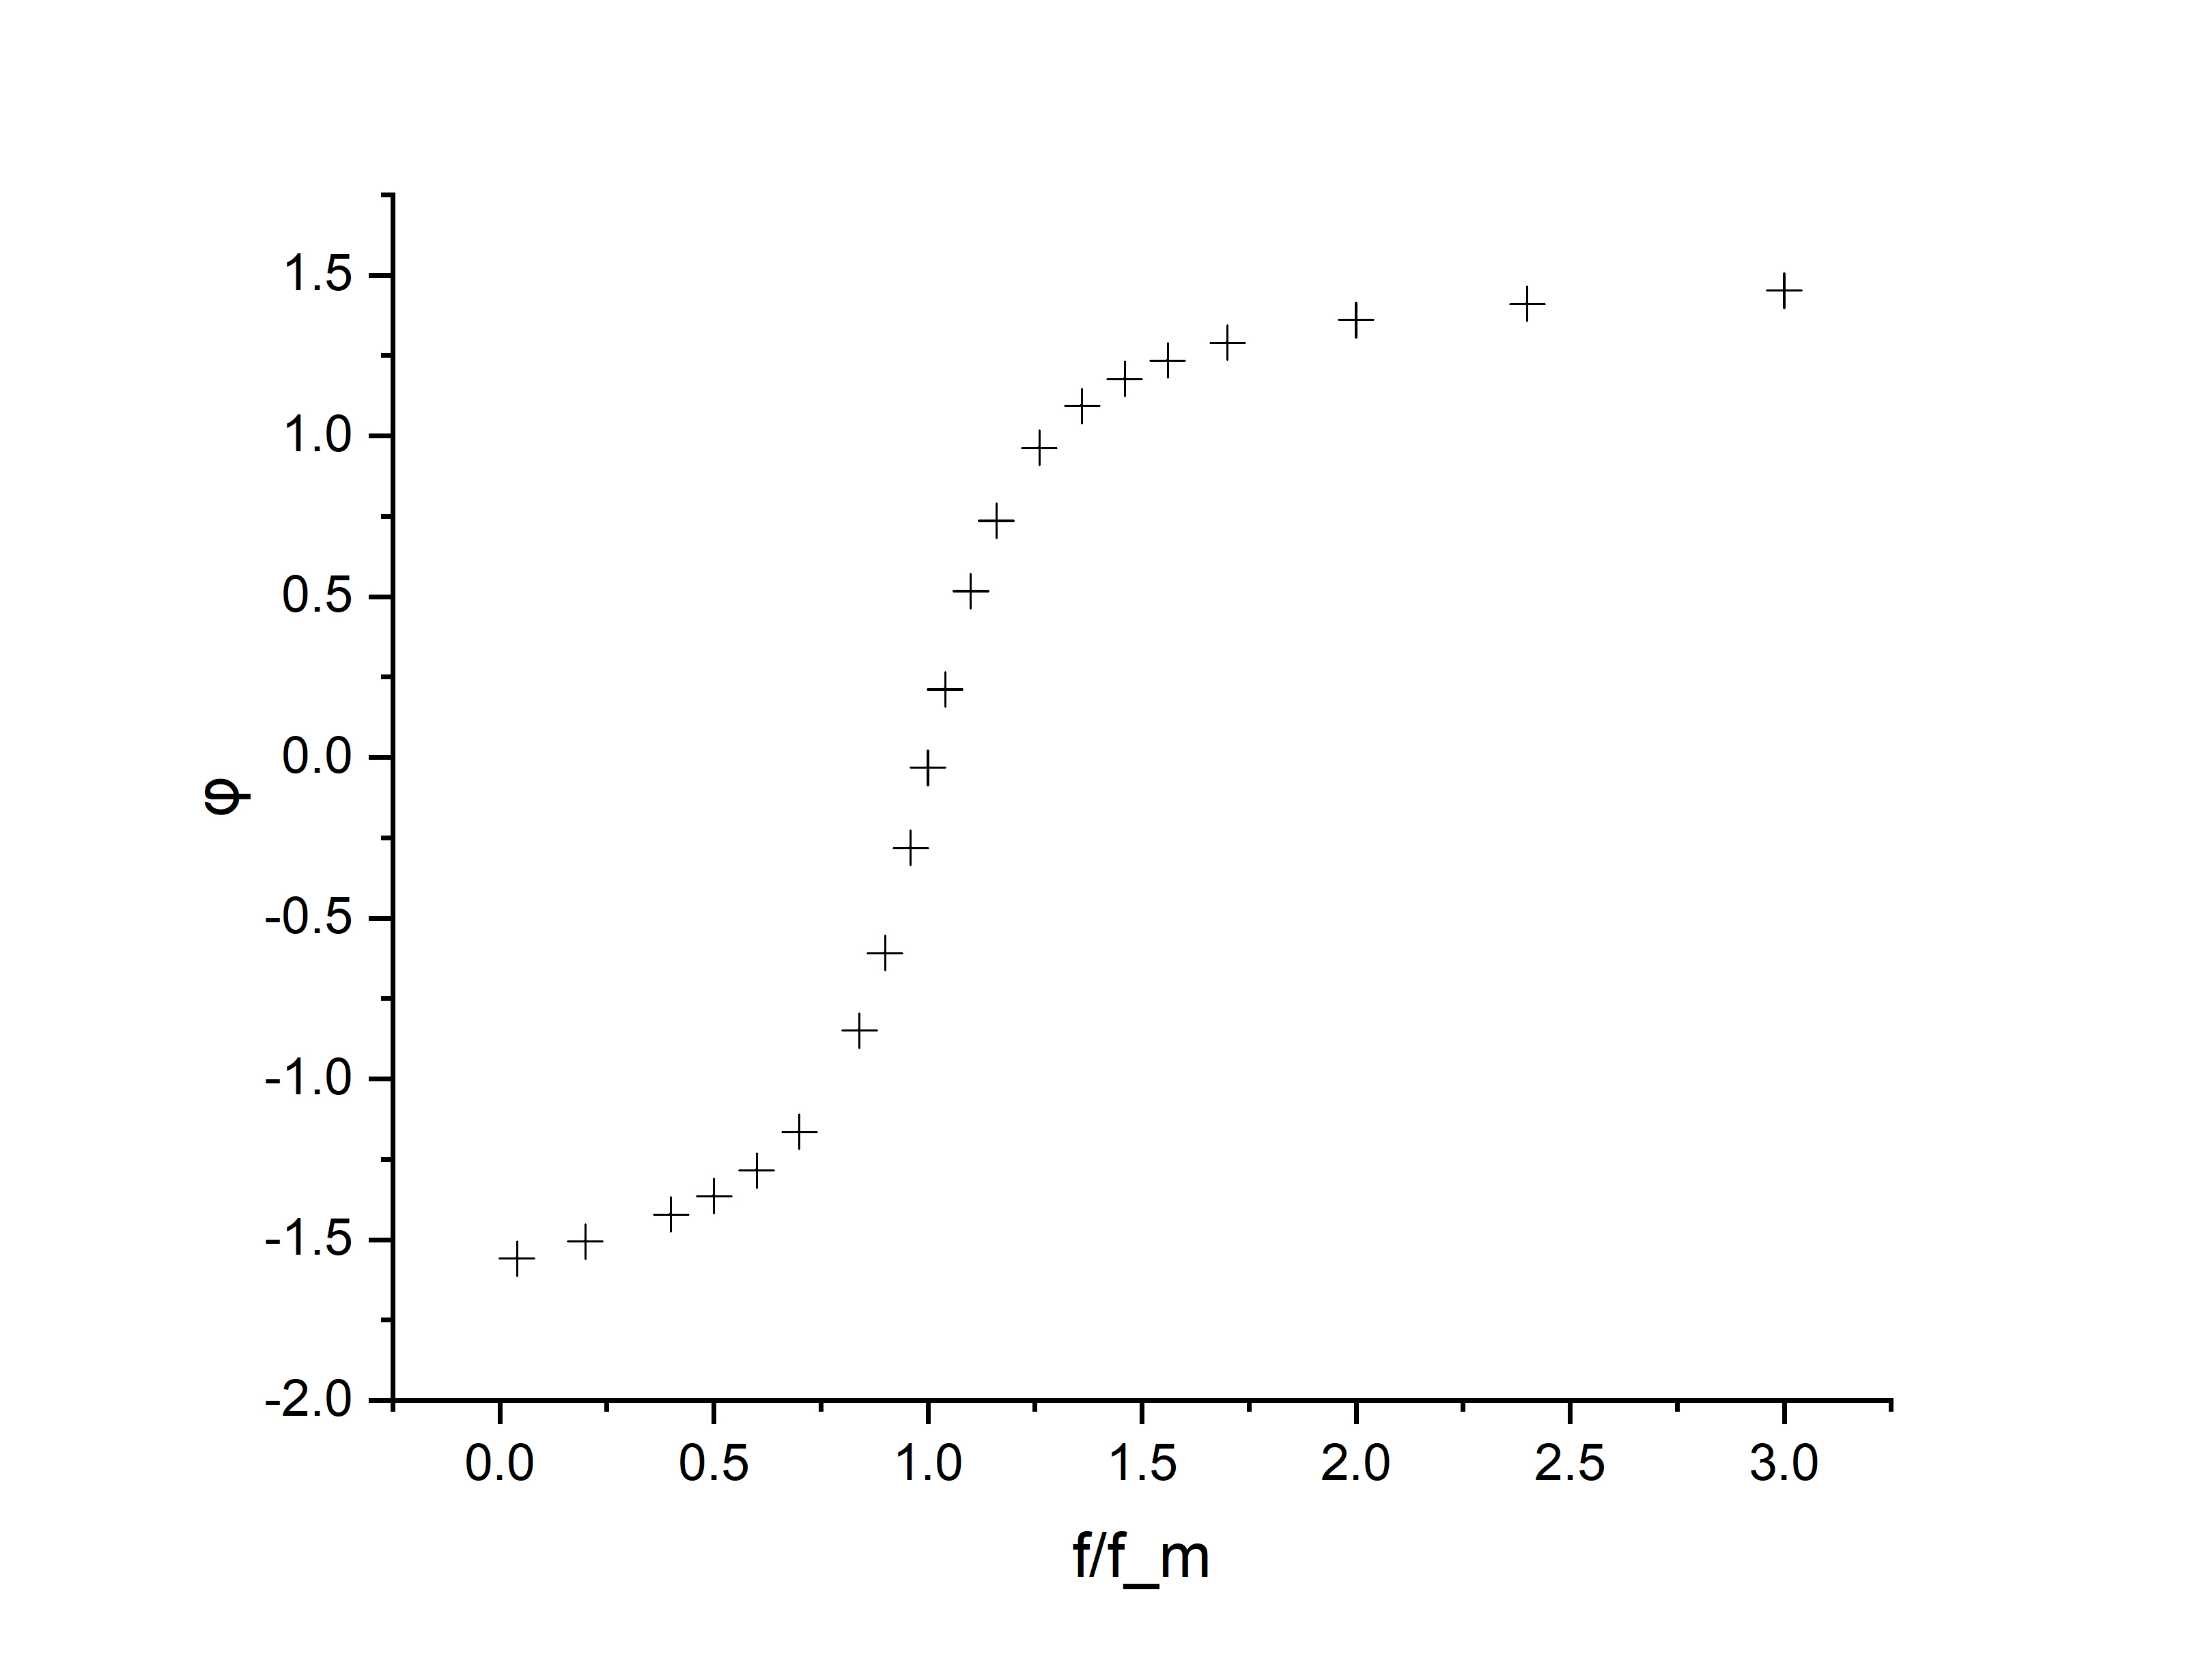
\includegraphics[width=12cm]{phase_t.jpg}
	\caption{Plot of Theoretic $\varphi_{theo}$ vs. $f/f_0$}
\end{figure}



The following is the experimentally calculated phase shift with respect to frequency ratio.

\begin{figure}[H]
	\center
	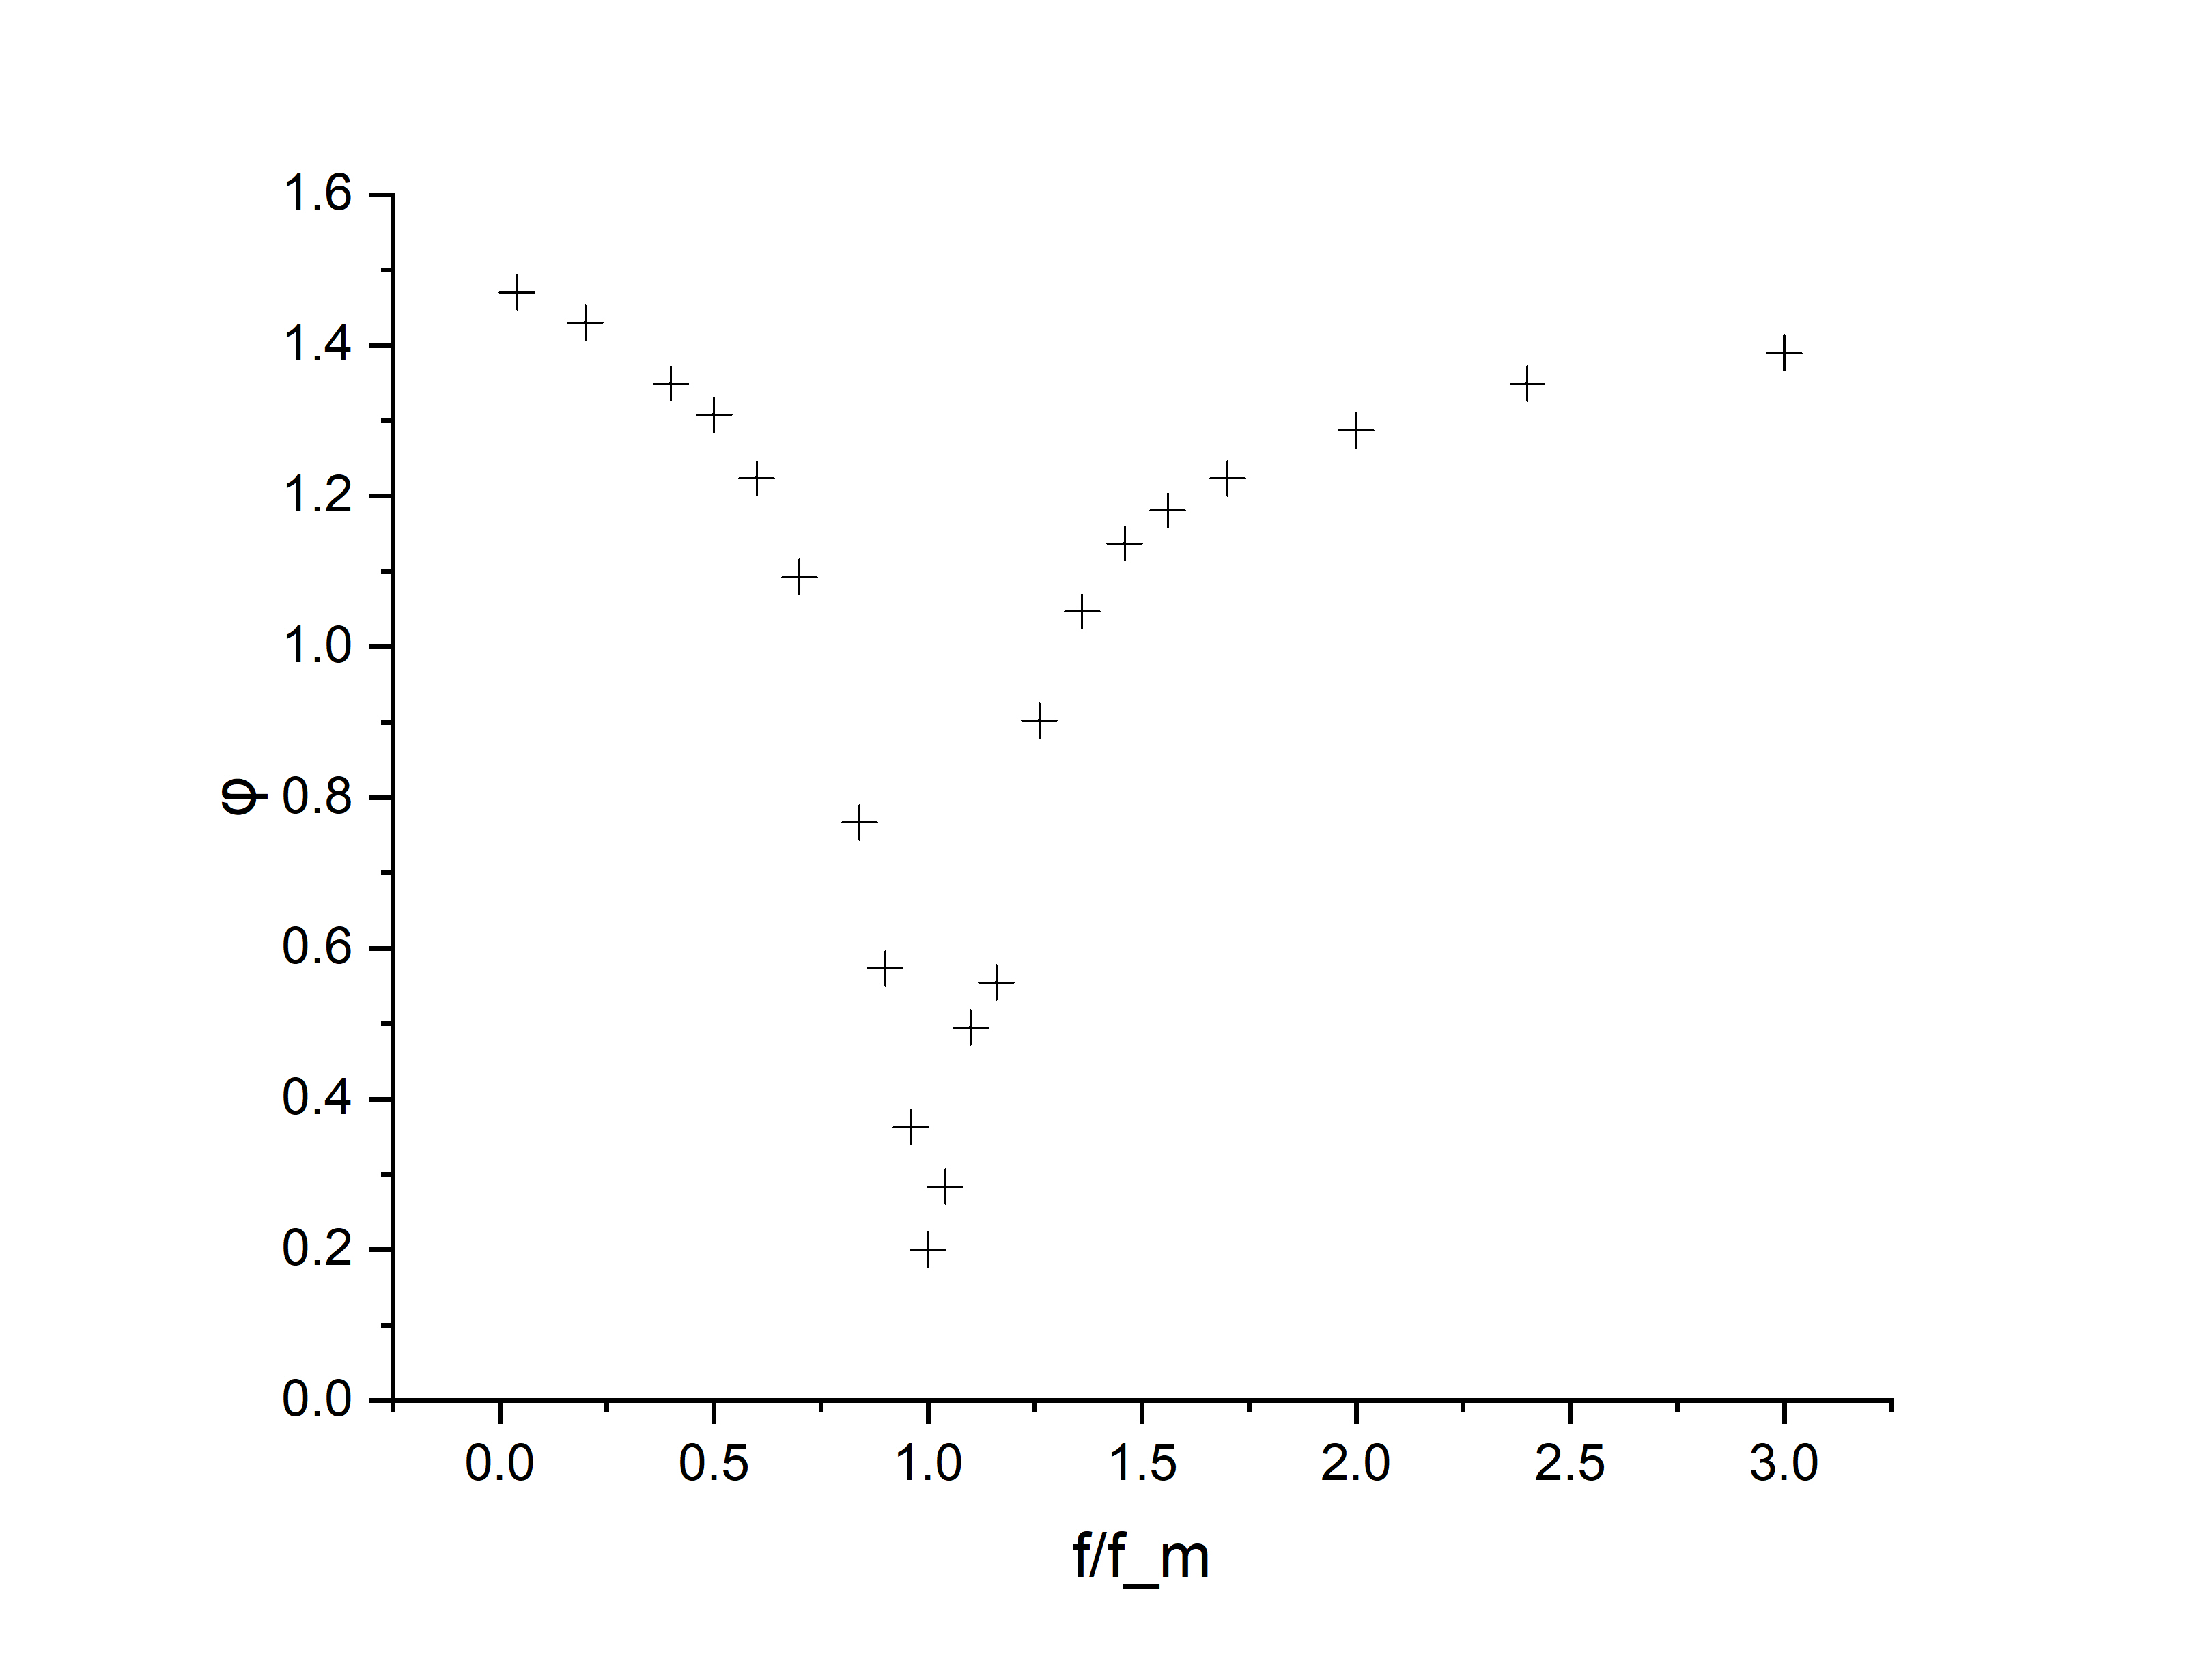
\includegraphics[width=10cm]{phase_e.jpg}
	\caption{Plot of Experimental $\varphi_{exp}$ vs. $f/f_0$}
\end{figure}

Note that all phase shift data retrieved are positive, because the formula we use
$$\varphi_{exp} = \tan^{-1}\bigg(\frac{\sqrt{\varepsilon^2-U_R^2}}{U_R}\bigg)$$
ensures it's positiveness by square roots. Thus, by applying the correct signs to the data, we can plot the correct graph as:

\begin{figure}[H]
	\center
	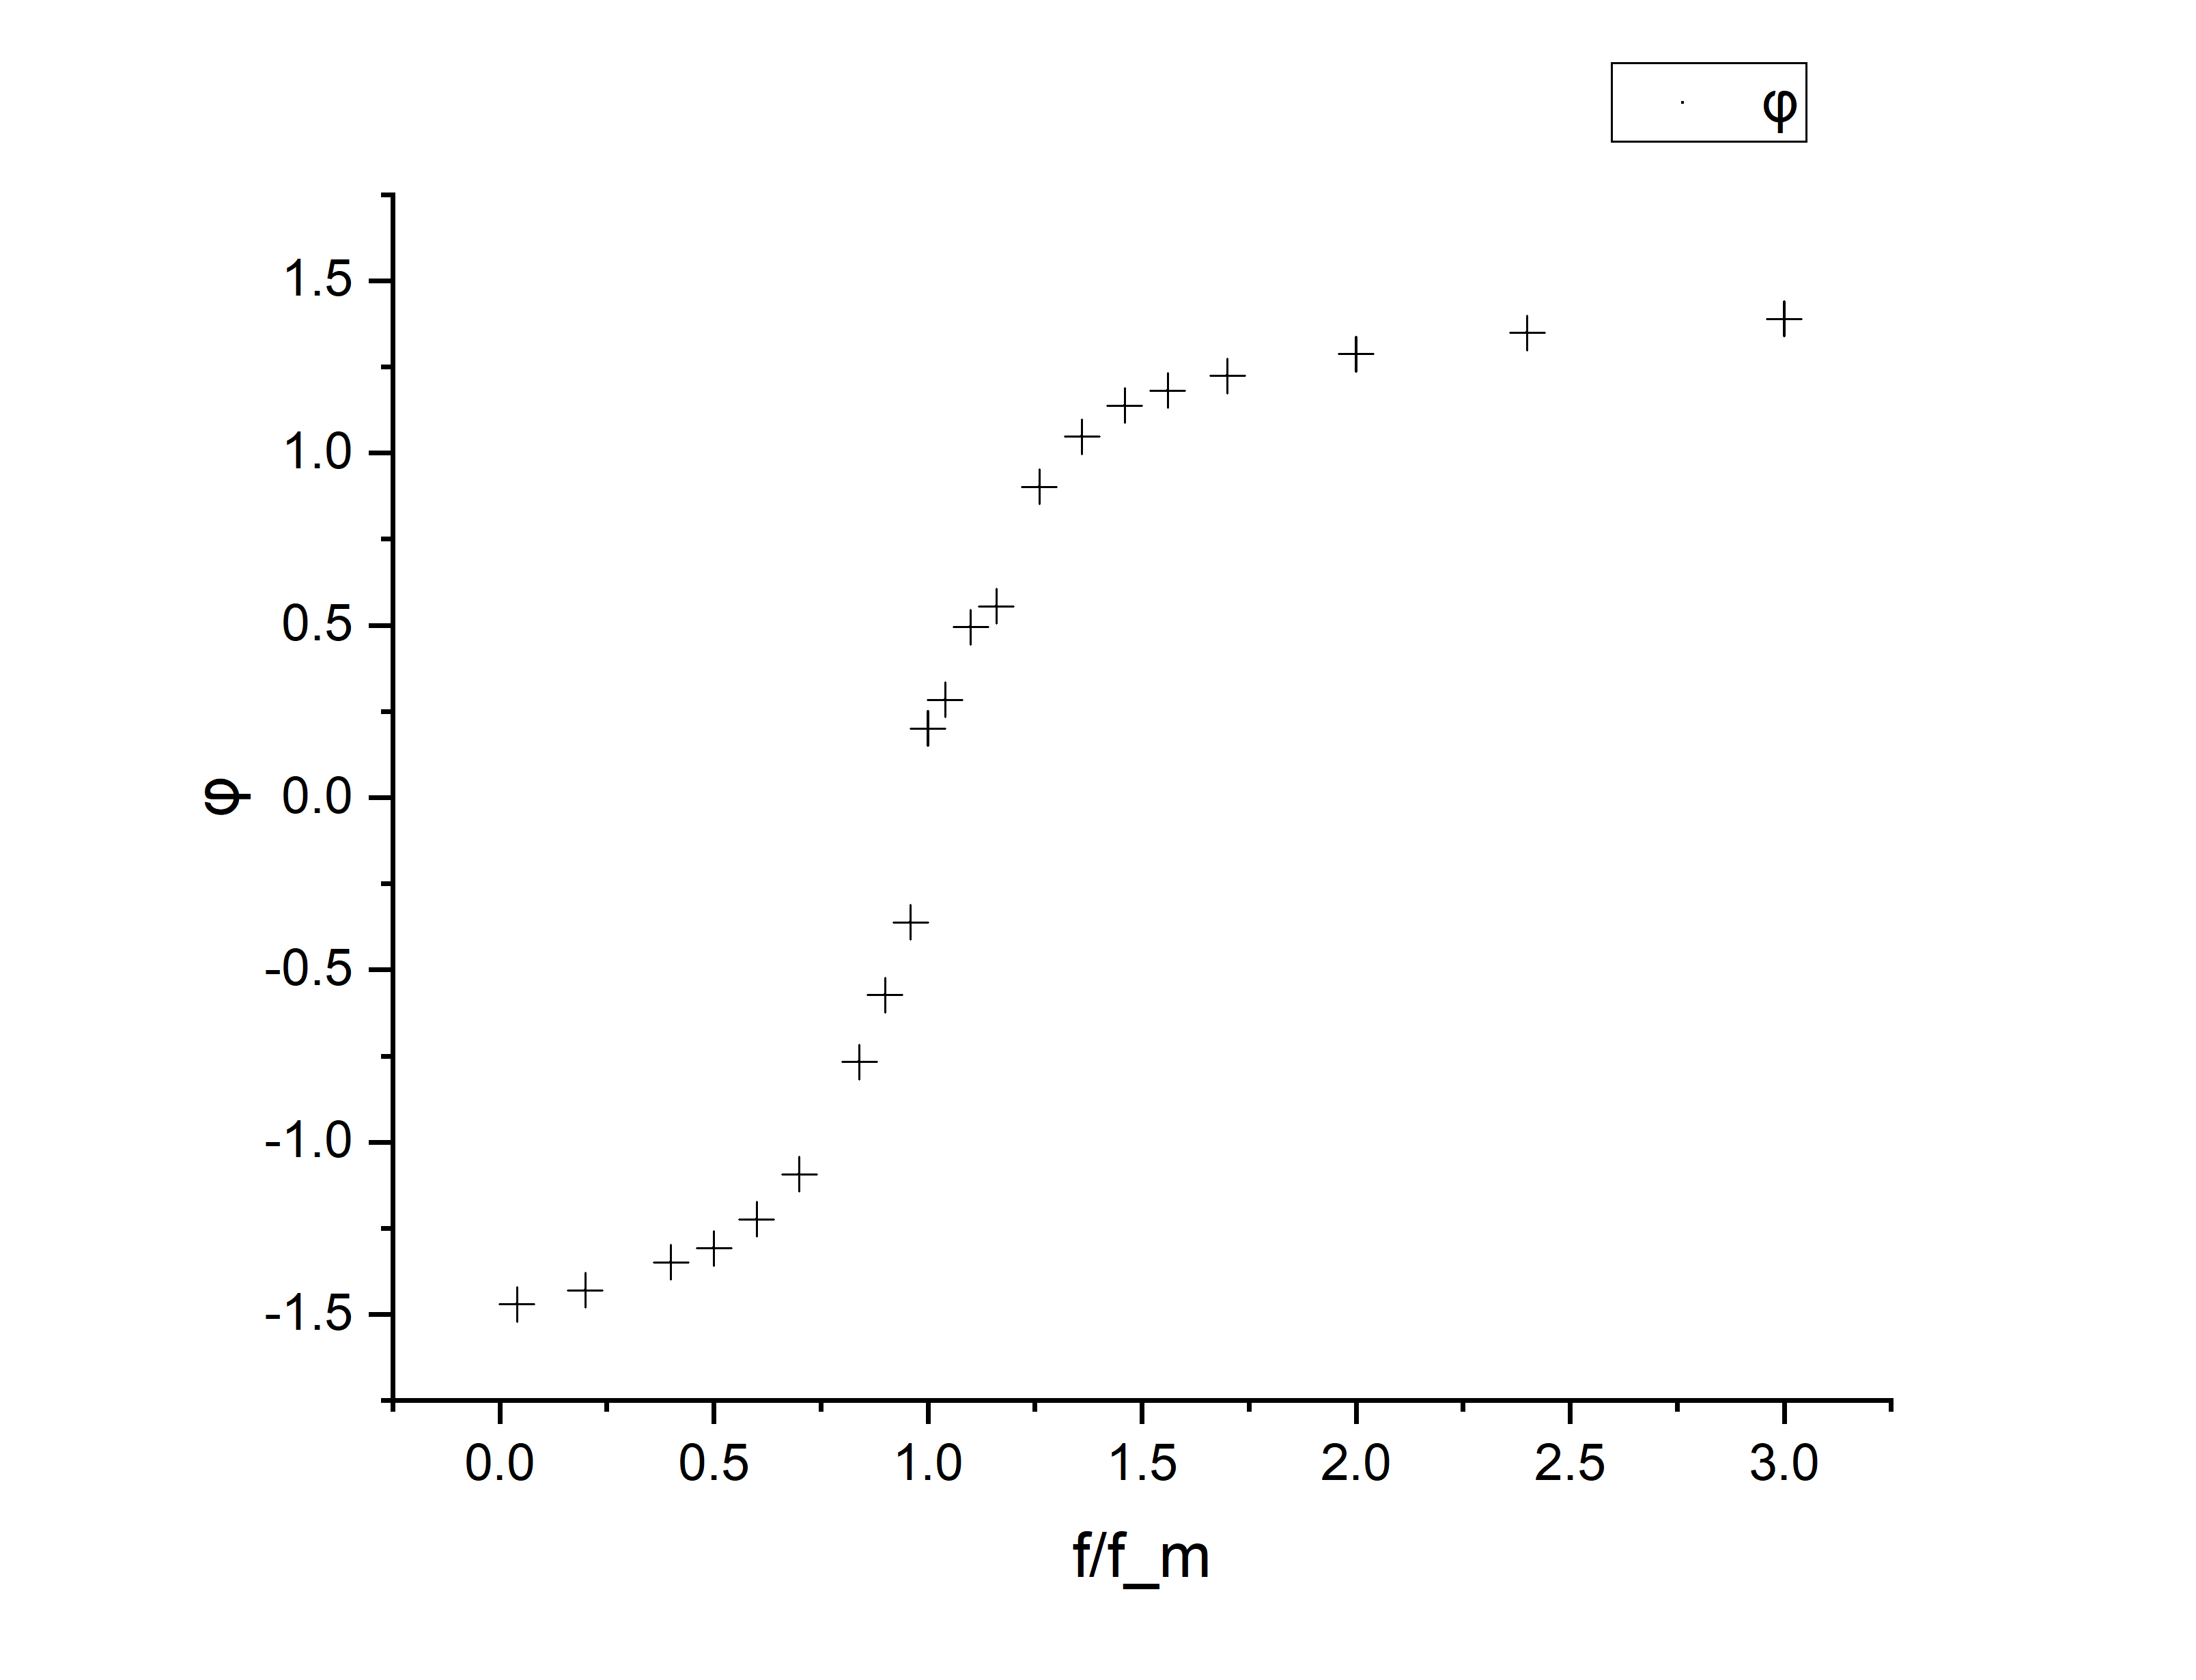
\includegraphics[width=10cm]{phase_e_ad.jpg}
	\caption{Plot of Experimental $\varphi_{exp}$ vs. $f/f_0$ (Adjusted).}
\end{figure}


From the following figures, we found the two plots match each other. Te experiment is successful.

\subsubsection{Calculation of Resonate Frequency $f_0$ and Quality Factor Q}

The theoretic resonate frequency $f_{0,theo}$ is determined by:
\begin{equation}
	f_{0,theo}=\frac{1}{2\pi \sqrt{LC}}
\end{equation}

Thus we can calculated it as
\begin{align*}
	f_{0,theo}
	 & =\frac{1}{2\pi \sqrt{LC}}                            \\
	 & =\frac{1}{2\pi\sqrt{0.01\times 1.0057\times10^{-7}}} \\
	 & =5018.6 \pm 0.2 [\text{Hz}]
\end{align*}

The experimental $f_0=5000.000$ [Hz], we can calculated the relative error $\delta$ by:

\begin{align*}
	\delta_{f_0}
	 & = \frac{f_{0,\text{ex}}-f_{0,\text{theo}}}{f_{0,\text{theo}}}\times 100\% \\
	 & = \frac{5018.6.000-5000}{5000}\times 100\%    \\
	 & = 0.372\%
\end{align*}

Then we calculate Quality Factor Q. Theoretically,
$$Q_{theo}=\frac{2\pi f_0 L}{R}$$
and experientially,
$$Q_{exp}=\frac{f_0}{f_2-f_1}$$

Thus,
\begin{align*}
	Q_{theo}
	 & =\frac{2\pi f_0 L}{R}                        \\
	 & =\frac{2\pi\times 5025.6\times 0.01}{100.15} \\
	 & =3.2670\pm 0.0003 [Hz]
\end{align*}

From the $U_R$ calculation, $U_R/\sqrt{2}=2.715$ [Vpp]. Thus, $f_2\approx 5800.000$[Hz] and $f_1\approx 4200.000$[Hz].

\begin{align*}
	Q_{exp}=\frac{f_0}{f_2-f_1}
	 & =\frac{5000.0000}{5800.00-4200.000} \\
	 & =3.125000\pm 0.000004 [Hz]
\end{align*}

we can calculated the relative error $\delta$ by:

\begin{align*}
	\delta_{Q}
	 & = \frac{Q_{exp}-Q_{theo}}{Q_{theo}}\times 100\% \\
	 & = \frac{3.125000-3.2670}{3.2670}\times 100\%    \\
	 & = -4.35\%
\end{align*}


\section{Uncertainty Analysis}

\subsection{Uncertainty of Data for RC Circuit}
The parameters, including resistance, frequency, Voltage $\varepsilon$, capacitance and time are all single measurement. They don't have a type-A uncertainty and, their type-B uncertainty can be calculated as their standard deviation. A sample calculation is

$$u_{R} = \Delta_{dev} = 1\times 10^{-2} [\Omega]$$

Thus, the uncertainty of the quantities are given by:
\begin{table}[!htbp]
	\centering
	\begin{tabular}{l c c}
		\hline
		                   & Value                  & Uncertainty        \\
		\hline
		R [$\Omega$]       & 100.15                 & 0.01               \\
		f [Hz]             & 1000.000               & 0.001              \\
		$\mathrm{E}$ [Vpp] & 4.000                  & 0.001              \\
		C [F]              & 1.0057$\times 10^{-7}$ & 1$\times 10^{-11}$ \\
		T$_{1/2}$ [s]      & 9.000$\times 10^{-6}$  & 1$\times 10^{-9}$  \\
		\hline
	\end{tabular}
	\caption{Uncertainty of all original data}
\end{table}

For the experimental time constant,
$$\tau_{exp} = \frac{T_{1/2}}{\ln 2}$$

We can find the uncertainty by:
\begin{align*}
	u_{\tau,exp}
	 & = \frac{\partial \tau}{\partial T_{1/2}}u_{T_{1/2}} \\
	 & = \frac{u_{T_{1/2}}}{\ln 2}                         \\
	 & = \frac{1\times 10^{-9}}{\ln 2}                     \\
	 & = 1.4\times 10^{-9}\,\,[\text{s}]
\end{align*}

For the theoretical time constant,
$$\tau_{\text{theo}} = RC$$

We can find the uncertainty by:

\begin{align*}
	u_{\tau,theo}
	 & = \sqrt{(\frac{\partial \tau}{\partial R}u_R)^2+(\frac{\partial \tau}{\partial C}u_C)^2} \\
	 & = \sqrt{(Cu_R)^2 + (Ru_C)^2}                                                             \\
	 & = \sqrt{(100.57\times 10^{-9}\times 0.01)^2 + (100.15 \times1\times 10^{-11})^2}         \\
	 & = 1.4\times 10^{-9}\,\,[\text{s}].
\end{align*}

\subsection{Uncertainty of Data for RL Circuit}
The parameters, including resistance, frequency, Voltage $\varepsilon$, inductance and time are all single measurement. They don't have a type-A uncertainty and, their type-B uncertainty can be calculated as their standard deviation. A sample calculation is

$$u_{R} = \Delta_{dev} = 1\times 10^{-2} [\Omega]$$

Thus, the uncertainty of the quantities are given by:
\begin{table}[!htbp]
	\centering
	\begin{tabular}{l c c}
		\hline
		                    & Value                 & Uncertainty       \\
		\hline
		R [$\Omega$]        & 100.15                & 0.01              \\
		f [Hz]              & 1000.000              & 0.001             \\
		$\varepsilon$ [Vpp] & 4.000                 & 0.001             \\
		L [H]               & 0.01                  & 0                 \\
		T$_{1/2}$ [s]       & 8.000$\times 10^{-5}$ & 1$\times 10^{-8}$ \\
		\hline
	\end{tabular}
	\caption{Transformed into SI units}
\end{table}

For the experimental time constant,
$$\tau_{exp} = \frac{T_{1/2}}{\ln 2}$$

We can find the uncertainty by:
\begin{align*}
	u_{\tau,exp}
	 & = \frac{\partial \tau}{\partial T_{1/2}}u_{T_{1/2}} \\
	 & = \frac{u_{T_{1/2}}}{\ln 2}                         \\
	 & = \frac{1\times 10^{-8}}{\ln 2}                     \\
	 & = 1.4\times 10^{-8}\,\,[\text{s}]
\end{align*}

For the experimental time constant,
$$\tau_{\text{theo}} = \frac{L}{R}$$

We can find the uncertainty by:

\begin{align*}
	u_{\tau,theo}
	 & = \sqrt{(\frac{\partial \tau}{\partial R}u_R)^2+(\frac{\partial \tau}{\partial L}u_L)^2} \\
	 & = \sqrt{(-\frac{Lu_R}{R^2})^2 + (\frac{u_L}{R})^2}                                       \\
	 & = \sqrt{(\frac{0.01\times 0.01}{100.15^2})^2 + (\frac{0}{100.15})^2}                     \\
	 & = 1.0\times 10^{-8}\,\,[\text{s}].
\end{align*}

\subsection{Uncertainty of Data for $RLC$ Circuit}

The parameters, including capacitance frequency, Voltage $\varepsilon$, inductance and time are all single measurement. They don't have a type-A uncertainty and, their type-B uncertainty can be calculated as their standard deviation. A sample calculation is

$$u_{f} = \Delta_{dev} = 1\times 10^{-3} [\Omega]$$

Thus, the uncertainty of the quantities are given by:
\begin{table}[!htbp]
	\centering
	\begin{tabular}{l c c}
		\hline
		                    & Value                  & Uncertainty        \\
		\hline
		f [Hz]              & 1000.000               & 0.001              \\
		$\varepsilon$ [Vpp] & 4.000                  & 0.001              \\
		C [F]               & 1.0057$\times 10^{-7}$ & 1$\times 10^{-11}$ \\
		L [H]               & 0.01                   & 0                  \\
		T$_{1/2}$ [s]       & 3.000$\times 10^{-5}$  & 1$\times 10^{-8}$  \\
		\hline
	\end{tabular}
	\caption{Transformed into SI units}
\end{table}

For the experimental time constant,
$$\tau = \frac{T_{1/2}}{\beta t}$$

We can find the uncertainty by:
\begin{align*}
	u_{\tau,\text{exp}}
	 & = \frac{\partial \tau}{\partial T_{1/2}}u_{T_{1/2}} \\
	 & = \frac{u_{T_{1/2}}}{1.68}                          \\
	 & = \frac{1\times 10^{-8}}{1.68}                      \\
	 & = 6\times 10^{-9}\,\,[\mu\text{s}]
\end{align*}

For the experimental time constant,
$$\tau = \sqrt{LC}$$

We can find the uncertainty by:

\begin{align*}
	u_{\tau,\text{theo}}
	 & = \sqrt{(\frac{\partial \tau_{\text{theo}}}{\partial L}u_L)^2 + (\frac{\partial \tau_{\text{theo}}}{\partial C}u_C)^2} \\
	 & = \sqrt{\bigg(\frac{1}{2}\sqrt{\frac{C}{L}}u_L\bigg)^2 + \bigg(\frac{1}{2}\sqrt{\frac{L}{C}}u_C\bigg)^2}               \\
	 & = \sqrt{0^2 + \bigg(\frac{1}{2}\sqrt{\frac{L}{C}}u_C\bigg)^2}                                                          \\
	 & = \frac{1}{2}\sqrt{\frac{L}{C}}u_C                                                                                     \\
	 & = \frac{1}{2}\sqrt{\frac{0.01}{1.0057\times10^{-7}}}\times 1 \times 10^{-11}                                           \\
	 & = 1.6\times 10^{-9}\,\,[\text{s}].
\end{align*}

\subsection{Uncertainty of Data for $RLC$ Resonant Circuit}

The parameters, including capacitance frequency, Voltage $\varepsilon$, inductance and time are all single measurement. They don't have a type-A uncertainty and, their type-B uncertainty can be calculated as their standard deviation. A sample calculation is

$$u_{f} = \Delta_{dev} = 1\times 10^{-3} [\Omega]$$

Thus, the uncertainty of the quantities are given by:

\begin{table}[!htbp]
	\centering
	\begin{tabular}{c|cc|cc}
		\hline
		   & $U_R$ [Vpp] & $u_u$ [Vpp] & $f$ [Hz] & $u_f$ [Hz] \\
		\hline
		1  & 0.520       & 0.001       & 1500.000 & 0.001      \\
		2  & 0.720       & 0.001       & 2000.000 & 0.001      \\
		3  & 0.960       & 0.001       & 2500.000 & 0.001      \\
		4  & 1.28        & 0.01        & 3000.000 & 0.001      \\
		5  & 1.68        & 0.01        & 3500.000 & 0.001      \\
		6  & 2.40        & 0.01        & 4000.000 & 0.001      \\
		7  & 2.68        & 0.01        & 4200.000 & 0.001      \\
		8  & 3.08        & 0.01        & 4400.000 & 0.001      \\
		9  & 3.44        & 0.01        & 4600.000 & 0.001      \\
		10 & 3.72        & 0.01        & 4800.000 & 0.001      \\
		11 & 3.84        & 0.01        & 5000.000 & 0.001      \\
		12 & 3.76        & 0.01        & 5200.000 & 0.001      \\
		13 & 3.56        & 0.01        & 5400.000 & 0.001      \\
		14 & 3.24        & 0.01        & 5600.000 & 0.001      \\
		15 & 2.96        & 0.01        & 5800.000 & 0.001      \\
		16 & 2.64        & 0.01        & 6000.000 & 0.001      \\
		17 & 2.12        & 0.01        & 6500.000 & 0.001      \\
		18 & 1.72        & 0.01        & 7000.000 & 0.001      \\
		19 & 1.48        & 0.01        & 7500.000 & 0.001      \\
		20 & 1.36        & 0.01        & 8000.000 & 0.001      \\
		21 & 1.16        & 0.01        & 8500.000 & 0.001      \\
		\hline
	\end{tabular}
	\caption{Uncertainty for the $U_R$ vs. $f$ dependence for a RLC resonant circuit}
\end{table}

\subsubsection{Uncertainty of $I/I_m$ vs. $f/f_m$ Relationship Data}

For $I/I_m = U_R/U_m$, its uncertainty is
\begin{align*}
	u_{I/I_m}
	 & = \sqrt{(\frac{\partial U_R/U_m}{\partial U_R}u_{U_R})^2 + (\frac{\partial U_R/U_m}{\partial U_m}u_{U_m})^2} \\
	 & = \sqrt{(\frac{u_{U_R}}{U_m})^2 + (-\frac{U_R}{U_m^2}u_{U_m})^2}
\end{align*}

For $f/f_0$, its uncertainty is calculated as
\begin{align*}
	u_{f/f_0}
	 & = \sqrt{(\frac{\partial f/f_0}{\partial f}u_f)^2 + (\frac{\partial f/f_0}{\partial f_0}u_{f_0})^2} \\
	 & = \sqrt{(\frac{u_f}{f_0})^2 + (-\frac{f}{f_0^2}u_{f_0})^2}                                         \\
\end{align*}

A sample calculation is provided by $\#$1.
\begin{align*}
	u_{I/I_m}
	 & = \sqrt{(\frac{u_{U_R}}{U_m})^2 + (-\frac{U_R}{U_m^2}u_{U_m})^2}      \\
	 & = \sqrt{(\frac{0.001}{3.84})^2 + (\frac{0.520}{3.84^2}\times 0.01)^2} \\
	 & = 0.0004
\end{align*}
\begin{align*}
	u_{f/f_0}
	 & = \sqrt{(\frac{u_f}{f_0})^2 + (-\frac{f}{f_0^2}u_{f_0})^2}                        \\
	 & = \sqrt{(\frac{0.001}{5000.000})^2 + (\frac{1500.000}{5000.000^2}\times 0.001)^2} \\
	 & = 2\times 10^{-7}
\end{align*}

By following the formula mentioned above we can calculate all the data samples, and they are listed in the following table.

\begin{table}[htbp]
	\centering
	\begin{tabular}{ccccccccc}
		\hline
		   & $U_R$ [Vpp] & $u_{U_R} [Vpp]$ & $f$ [Hz] & $u_f$ [Hz] & $I/I_m$ & $u_{I/I_m}$ & $f/f_m$   & $u_{f/f_m}$ \\
		\hline
		1  & 0.520       & 0.001           & 1500.000 & 0.001      & 0.1354  & 0.0004      & 0.3000000 & 0.0000002   \\
		2  & 0.720       & 0.001           & 2000.000 & 0.001      & 0.1875  & 0.0006      & 0.4000000 & 0.0000002   \\
		3  & 0.960       & 0.001           & 2500.000 & 0.001      & 0.2500  & 0.0007      & 0.5000000 & 0.0000002   \\
		4  & 1.28        & 0.01            & 3000.000 & 0.001      & 0.333   & 0.003       & 0.6000000 & 0.0000002   \\
		5  & 1.68        & 0.01            & 3500.000 & 0.001      & 0.438   & 0.003       & 0.7000000 & 0.0000002   \\
		6  & 2.40        & 0.01            & 4000.000 & 0.001      & 0.625   & 0.003       & 0.8000000 & 0.0000003   \\
		7  & 2.68        & 0.01            & 4200.000 & 0.001      & 0.698   & 0.003       & 0.8400000 & 0.0000003   \\
		8  & 3.08        & 0.01            & 4400.000 & 0.001      & 0.802   & 0.003       & 0.8800000 & 0.0000003   \\
		9  & 3.44        & 0.01            & 4600.000 & 0.001      & 0.896   & 0.003       & 0.9200000 & 0.0000003   \\
		10 & 3.72        & 0.01            & 4800.000 & 0.001      & 0.969   & 0.004       & 0.9600000 & 0.0000003   \\
		11 & 3.84        & 0.01            & 5000.000 & 0.001      & 1.000   & 0.004       & 1.0000000 & 0.0000003   \\
		12 & 3.76        & 0.01            & 5200.000 & 0.001      & 0.979   & 0.004       & 1.0400000 & 0.0000003   \\
		13 & 3.56        & 0.01            & 5400.000 & 0.001      & 0.927   & 0.004       & 1.0800000 & 0.0000003   \\
		14 & 3.24        & 0.01            & 5600.000 & 0.001      & 0.844   & 0.003       & 1.1200000 & 0.0000003   \\
		15 & 2.96        & 0.01            & 5800.000 & 0.001      & 0.771   & 0.003       & 1.1600000 & 0.0000003   \\
		16 & 2.64        & 0.01            & 6000.000 & 0.001      & 0.688   & 0.003       & 1.2000000 & 0.0000003   \\
		17 & 2.12        & 0.01            & 6500.000 & 0.001      & 0.552   & 0.003       & 1.3000000 & 0.0000003   \\
		18 & 1.72        & 0.01            & 7000.000 & 0.001      & 0.448   & 0.003       & 1.4000000 & 0.0000003   \\
		19 & 1.48        & 0.01            & 7500.000 & 0.001      & 0.385   & 0.003       & 1.5000000 & 0.0000004   \\
		20 & 1.36        & 0.01            & 8000.000 & 0.001      & 0.354   & 0.003       & 1.6000000 & 0.0000004   \\
		21 & 1.16        & 0.01            & 8500.000 & 0.001      & 0.302   & 0.003       & 1.7000000 & 0.0000004   \\
		\hline
	\end{tabular}
	\caption{Relationship of $I/I_m$ vs. $f/f_0$}
	\label{table::frequency}
\end{table}

\subsubsection{Uncertainty of Phase Shift Analysis}

For $\varphi_\text{theo} = \tan^{-1}\bigg(\frac{2\pi fL-\frac{1}{2\pi fC}}{R}\bigg)$, the uncertainty

\begin{align*}
	u_{\varphi_\text{theo}} & = \sqrt{(\frac{\partial \varphi_\text{theo}}{\partial f}u_f)^2 + (\frac{\partial \varphi_\text{theo}}{\partial C}u_C)^2 + (\frac{\partial \varphi_\text{theo}}{\partial R}u_R)^2}                                                                                                                                               \\
	                        & = \sqrt{\left( \frac{R\big(2\pi L +\frac{1}{2\pi f^2 C}\big)}{R^2 + \big(2\pi fL - \frac{1}{2\pi fC}\big)^2} u_f \right)^2 + \left( \frac{R}{2\pi fC^2\big[R^2+\big(2\pi fL - \frac{1}{2\pi fC}\big)^2\big]} u_C \right)^2 + \left(-\frac{2\pi fL-\frac{1}{2\pi fC}}{R^2+\big(2\pi fL-\frac{1}{2\pi fC}\big)^2} u_R \right)^2}.
\end{align*}

Take the first set of data as an example,

\begin{align*}
	u_{\varphi_\text{theo}} = & \sqrt{\left( \frac{100.15\times\big(2\pi\times0.01 +\frac{1}{2\pi\times 1500^2\times 100.57}\big)}{100.15^2 + \big(2\pi\times 1500\times 0.01 - \frac{1}{2\pi\times 1500\times 100.57}\big)^2}\times 0.001 \right)^2 +} \\
	                          & \overline{\left( \frac{100.15}{2\pi\times 1500\times 100.57^2 \times \big[100.15^2+\big(2\pi\times1500\times 0.01 - \frac{1}{2\pi\times1500\times100.57}\big)^2\big]} \right)^2 +}                                      \\
	                          & \overline{\left( \frac{2\pi\times 1500\times0.01-\frac{1}{2\pi\times 1500\times 100.57}}{100.15^2+\big(2\pi\times 1500\times0.01-\frac{1}{2\pi\times 1500\times 100.57}\big)^2} \right)^2}                              \\
	                          & = 0.00011\,[\text{rad}].
\end{align*}

The uncertainties for other sets of data are calculated in the same way and the results are shown in Table \ref{table::phase_shift}.

For $\varphi_{exp} = \tan^{-1}\bigg(\frac{\sqrt{\varepsilon^2-U_R^2}}{U_R}\bigg)$, its uncertainty is

$$u_{\varphi,e} = (\frac{\partial \varphi_e}{\partial U_R}u_{U_R})^2 $$
Calculate the partial derivative:
$$\frac{\partial \varphi_e}{\partial U_R}=\frac{1}{\sqrt{\varepsilon^2-U_R^2}}$$
Thus,
$$u_{\varphi,e} = (\frac{u_{U_R}}{\sqrt{\varepsilon^2-U_R^2}})^2 $$

Thus, a sample calculation of $\#$1 is provided as follows.
\begin{align*}
	u_{\varphi,e}
	 & = (\frac{u_{U_R}}{\sqrt{\varepsilon^2-U_R^2}})^2 \\
	 & = (\frac{0.01}{\sqrt{4.000^2-0.520^2}})^2        \\
	 & = 0.000006 [\text{Hz}]
\end{align*}

\begin{align*}
	\frac{\partial \varphi_t}{\partial f}
	 & = \frac{R\big(2\pi L +\frac{1}{2\pi f^2 C}\big)}{R^2 + \big(2\pi fL - \frac{1}{2\pi fC}\big)^2}                                                                                                                                       \\
	 & = \frac{100.15\times \big(2\pi \times 0.01 +\frac{1}{2\pi\times (1500.000)^2\times (1.0057\times 10^{-7})}\big)}{(100.15)^2 + \big(2\pi \times 1500.000\times 0.01 - \frac{1}{2\pi\times 1500.000\times 1.0057\times 10^{-7}}\big)^2} \\
	 & = 6.35003\times 10^{-5}
\end{align*}

\begin{align*}
	\frac{\partial \varphi_t}{\partial C}
	 & = \frac{R}{2\pi fC^2\big[R^2+\big(2\pi fL - \frac{1}{2\pi fC}\big)^2\big]}                                                                                                                   \\
	 & = \frac{100.15}{2\pi \times 1500.00\times (1.0057\times 10^{-7})^2\big[(100.15)^2+\big(2\pi \times 1500.000\times 0.01 - \frac{1}{2\times 1500.00\times (1.0057\times 10^{-7})}\big)^2\big]} \\
	 & = 126433.1015
\end{align*}

\begin{align*}
	\frac{\partial \varphi_t}{\partial R}
	 & = -\frac{2\pi fL-\frac{1}{2\pi fC}}{R^2+\big(2\pi fL-\frac{1}{2\pi fC}\big)^2}                                                                                                                                      \\
	 & = -\frac{2\pi\times 1500.00 \times 0.01-\frac{1}{2\pi \times 1500.000\times 1.0057\times 10^{-7}}}{(100.15)^2+\big(2\pi\times 1500.000\times 0.01-\frac{1}{2\pi \times 1500.000\times 1.0057\times 10^{-7}}\big)^2} \\
	 & = 0.000126208
\end{align*}
And thus
\begin{align*}
	u_{\varphi,t}
	 & = \sqrt{(\frac{\partial \varphi_t}{\partial f}u_f)^2 + (\frac{\partial \varphi_t}{\partial C}u_C)^2 + (\frac{\partial \varphi_t}{\partial R}u_R)^2} \\
	 & = \sqrt{(6.35003\times 10^{-5}\times 0.001)^2 + (126433.1015\times 1\times 10^{-11})^2 + (0.000126208 \times 0.01)^2}                               \\
	 & = 0.0004   [\text{Hz}]
\end{align*}


The uncertainties for other sets of data are calculated in the same way and the results are shown in Table \ref{table::phase_shift}.

By using the above calculation we can get:
\begin{table}[!htbp]
	\centering
	\begin{tabular}{cccccc}
		\hline
		$f/f_0$   & $u_{f/f_0}$ & $\varphi_{\text{theo}}$ & $u_{\varphi_{\text{theo}}}$ & $\varphi_{\text{ex}}$ & $u_{\varphi_{\text{ex}}}$ \\
		\hline
		0.3000000 & 0.0000002   & -1.46693                & 0.00011                     & 1.4350                & 0.0004                    \\
		0.4000000 & 0.0000002   & -1.4215                 & 0.0002                      & 1.3822                & 0.0006                    \\
		0.5000000 & 0.0000002   & -1.3634                 & 0.0003                      & 1.3181                & 0.0007                    \\
		0.6000000 & 0.0000002   & -1.2836                 & 0.0004                      & 1.231                 & 0.003                     \\
		0.7000000 & 0.0000002   & -1.1637                 & 0.0007                      & 1.118                 & 0.003                     \\
		0.8000000 & 0.0000003   & -0.9641                 & 0.0013                      & 0.896                 & 0.004                     \\
		0.8400000 & 0.0000003   & -0.845                  & 0.002                       & 0.798                 & 0.004                     \\
		0.8800000 & 0.0000003   & -0.693                  & 0.002                       & 0.640                 & 0.006                     \\
		0.9200000 & 0.0000003   & -0.502                  & 0.003                       & 0.460                 & 0.008                     \\
		0.9600000 & 0.0000003   & -0.274                  & 0.003                       & 0.251                 & 0.015                     \\
		1.0000000 & 0.0000003   & -0.023                  & 0.003                       & 0                     & /                         \\
		1.0400000 & 0.0000003   & 0.220                   & 0.003                       & 0.20                  & 0.02                      \\
		1.0800000 & 0.0000003   & 0.432                   & 0.002                       & 0.384                 & 0.009                     \\
		1.1200000 & 0.0000003   & 0.605                   & 0.002                       & 0.567                 & 0.006                     \\
		1.1600000 & 0.0000003   & 0.7407                  & 0.0015                      & 0.691                 & 0.005                     \\
		1.2000000 & 0.0000003   & 0.8466                  & 0.0012                      & 0.813                 & 0.004                     \\
		1.3000000 & 0.0000003   & 1.0251                  & 0.0007                      & 0.986                 & 0.004                     \\
		1.4000000 & 0.0000003   & 1.1326                  & 0.0004                      & 1.106                 & 0.003                     \\
		1.5000000 & 0.0000004   & 1.2034                  & 0.0003                      & 1.175                 & 0.003                     \\
		1.6000000 & 0.0000004   & 1.2534                  & 0.0002                      & 1.209                 & 0.003                     \\
		1.7000000 & 0.0000004   & 1.29050                 & 0.00014                     & 1.264                 & 0.003                     \\
		\hline
	\end{tabular}%
	\caption{Uncertainty of Theoretic and experimental phase shift vs. frequency ratio}
	\label{table::phase_shift}
\end{table}

\subsubsection{Uncertainty for Resonant Frequency $f_0$ and Quality Factor Q}

The theoretic resonant frequency is
$$f_{0,theo}=\frac{1}{2\pi \sqrt{LC}}$$

Thus, its uncertainty can be calculated by
\begin{align*}
	u_{f_0,theo}
	 & = \sqrt{(\frac{\partial f}{\partial L}u_{L})^2+(\frac{\partial f}{\partial C}u_{C})^2}                                                                                                  \\
	 & = \sqrt{(-\frac{C}{4\pi (LC)^{1.5}} u_{L})^2+(-\frac{L}{4\pi (LC)^{1.5}} u_{C})^2}                                                                                                      \\
	 & = \sqrt{(-\frac{1.0057\times 10^{-7}}{4\pi (0.01\times 1.0057\times 10^{-7})^{1.5}} \times 0)^2+(-\frac{0.01}{4\pi (0.01\times 1.0057\times 10^{-7})^{1.5}} \times 1\times 10^{-11})^2} \\
	 & = 0.3\,\,[\text{Hz}]
\end{align*}

Then we calculated the uncertainty of the quality factor. Theoretically, the uncertainty of the quality factor $Q$ is
\begin{align*}
	u_{Q,t}
	 & = \sqrt{(\frac{\partial Q_{\text{theo}}}{\partial R}u_R)^2 + (\frac{\partial Q_{\text{theo}}}{\partial C}u_C)^2}                                                                                                                        \\
	 & = \sqrt{(-\frac{\sqrt{LC}}{R^2C}u_R)^2 + (-\frac{\sqrt{L}}{2RC^{-1.5}} u_C)^2}                                                                                                                                                          \\
	 & = \sqrt{\bigg(-\frac{\sqrt{0.01\times 1.0057\times 10^{-11}}}{100.15^2\times 1.0057\times 10^{-11}}\times 0.01\bigg)^2 + \bigg(-\frac{\sqrt{0.01}}{2\times 100.15\times(1.0057\times 10^{-11})^{-1.5}}\times 1 \times 10^{-11}\bigg)^2} \\
	 & = 3\times 10^{-4}
\end{align*}

To find the quality factor, first find out the frequencies $f_1$, $f_2$ at which $I/I_m$ is about $1/\sqrt{2}$. Consulting Table \ref{table::frequency}, we obtain that $f_1 = 4200 \text{Hz}$ and $f_2 = 5800 \text{Hz}$. Then, according to Eq.\eqref{eq:Qex}, the experimental quality factor

Experimentally, The uncertainty of the quality factor $Q$ is
\begin{align*}
	u_{Q,e}
	 & = \sqrt{(\frac{\partial Q}{\partial f_0}u_{f_0})^2 + (\frac{\partial Q}{\partial f_1}u_{f_1})^2 + (\frac{\partial Q}{\partial f_2}u_{f_2})^2}                                                \\
	 & = \sqrt{\bigg(\frac{u_{f_0}}{f_2-f_1}\bigg)^2 + \bigg(\frac{f_0}{(f_2-f_1)^2}u_{f_1}\bigg)^2 + \bigg(-\frac{f_0}{(f_2-f_1)^2}u_{f_2}\bigg)^2}                                                \\
	 & = \sqrt{\bigg(\frac{0.001}{5800.000-4200.000}\bigg)^2 + \bigg(\frac{5000.000}{(5800.000-4200.000)^2}\times0.001\bigg)^2  + \bigg(-\frac{5000.000}{(5800.000-4200.000)^2}\times0.001\bigg)^2} \\
	 & = 4 \times 10^{-6}
\end{align*}


\section{Conclusion and Discussion}

\subsection{Conclusion}

In exercise 5, we generally studied the properties of alternating-current circuits, especially, the processes of charging and discharging of capacitors, the phenomenon of electromagnetic induction in inductive elements. 

In terms of ability to be developed, we obtained acquaintance of the methods for measuring the amplitude-frequency and the phase-frequency characteristics of $RC$, $RL$, and $RLC$ series circuits. 

The following is a conclusion of the whole experiment.

By applying $T_{1/2}$ measuring, we experimentally determined the time constants of RC, RL and critically damped RCL circuits. The following is the results.

\begin{table}[!htbp]
\centering
\begin{tabular}{c c c c}
\hline
& Experimental $\tau\,\,[\mu\text{s}]$ & Theoretical $\tau_{\text{theo}}\,\,[\mu\text{s}]$ & Relative error\\
\hline
$RC$ circuit & 12.9843 $\pm$ 0.0014 & 10.0721$\pm$ 0.0014 & 28.91$\%$\\
$RL$ circuit & 115.4156 $\pm$ 0.0014 & 99.8502 $\pm$ 0.0014 & 15.59$\%$\\
$RLC$ circuit & 17.857 $\pm$ 0.014 & 31.713 $\pm$ 0.010 & -43.69$\%$\\
\hline
\end{tabular}
\caption{Result of time constant in $RC$, $RL$ and critically damped $RLC$ series circuits}
\end{table}

The relative errors are relatively huge, and the reasons of errors will be discussed in DISCUSSION part.

\subsection{Discussion}

Here we will discuss the problems in this exercise, some potential errors which may lead to huge variation, and some suggestions.

\subsubsection{System Errors}

\begin{itemize}
\item In principle, the way $f_1$ and $f_2$ are found is not accurate.

We cannot find the corresponding $f$ for $U_R/\sqrt{2}$. The estimation will lead to a difference of around 200[Hz]. This will cause significant errors.
\item Inner resistance causes errors.

In ideal condition, the inner resistance of the circuit wire, inductor and the capacitor is ignore. However, this is not the case. For RC and RL circuits, the inner resistance will cause a higher $R_{eq}$, giving a higher time constant $\tau$. Also, in resonance circuits, the measured $U_R$ will be smaller because voltage division.
\end{itemize}

\subsubsection{Random Errors}

\begin{itemize}
\item Lissajous figures are always vibrating, and it's not a good way to judge whether the wave is in phase. 
\item The oscilloscope is not steady when we did the experiment. The readings are always vibrating.
\item The oscilloscope's cursor is not precise enough. First, it can't reach exactly $T_{1/2}$ sometimes. Also, the judge is based on human eyes, which is not accurate.
\item Due to some signal failure, although voltage is generated from function generators, the frequency is not exactly as the one in the function generator than in the oscilloscope, usually a $\pm 0.5\%$ relative difference.
\end{itemize}

\subsubsection{Improvements}

\begin{itemize}
\item Lissajous figures are always vibrating, and it's not a good way to judge whether the wave is in phase. Instead, comparing directly the waves by adjusting the vertical scale is more accurate.

\begin{figure}[!htbp]
\center
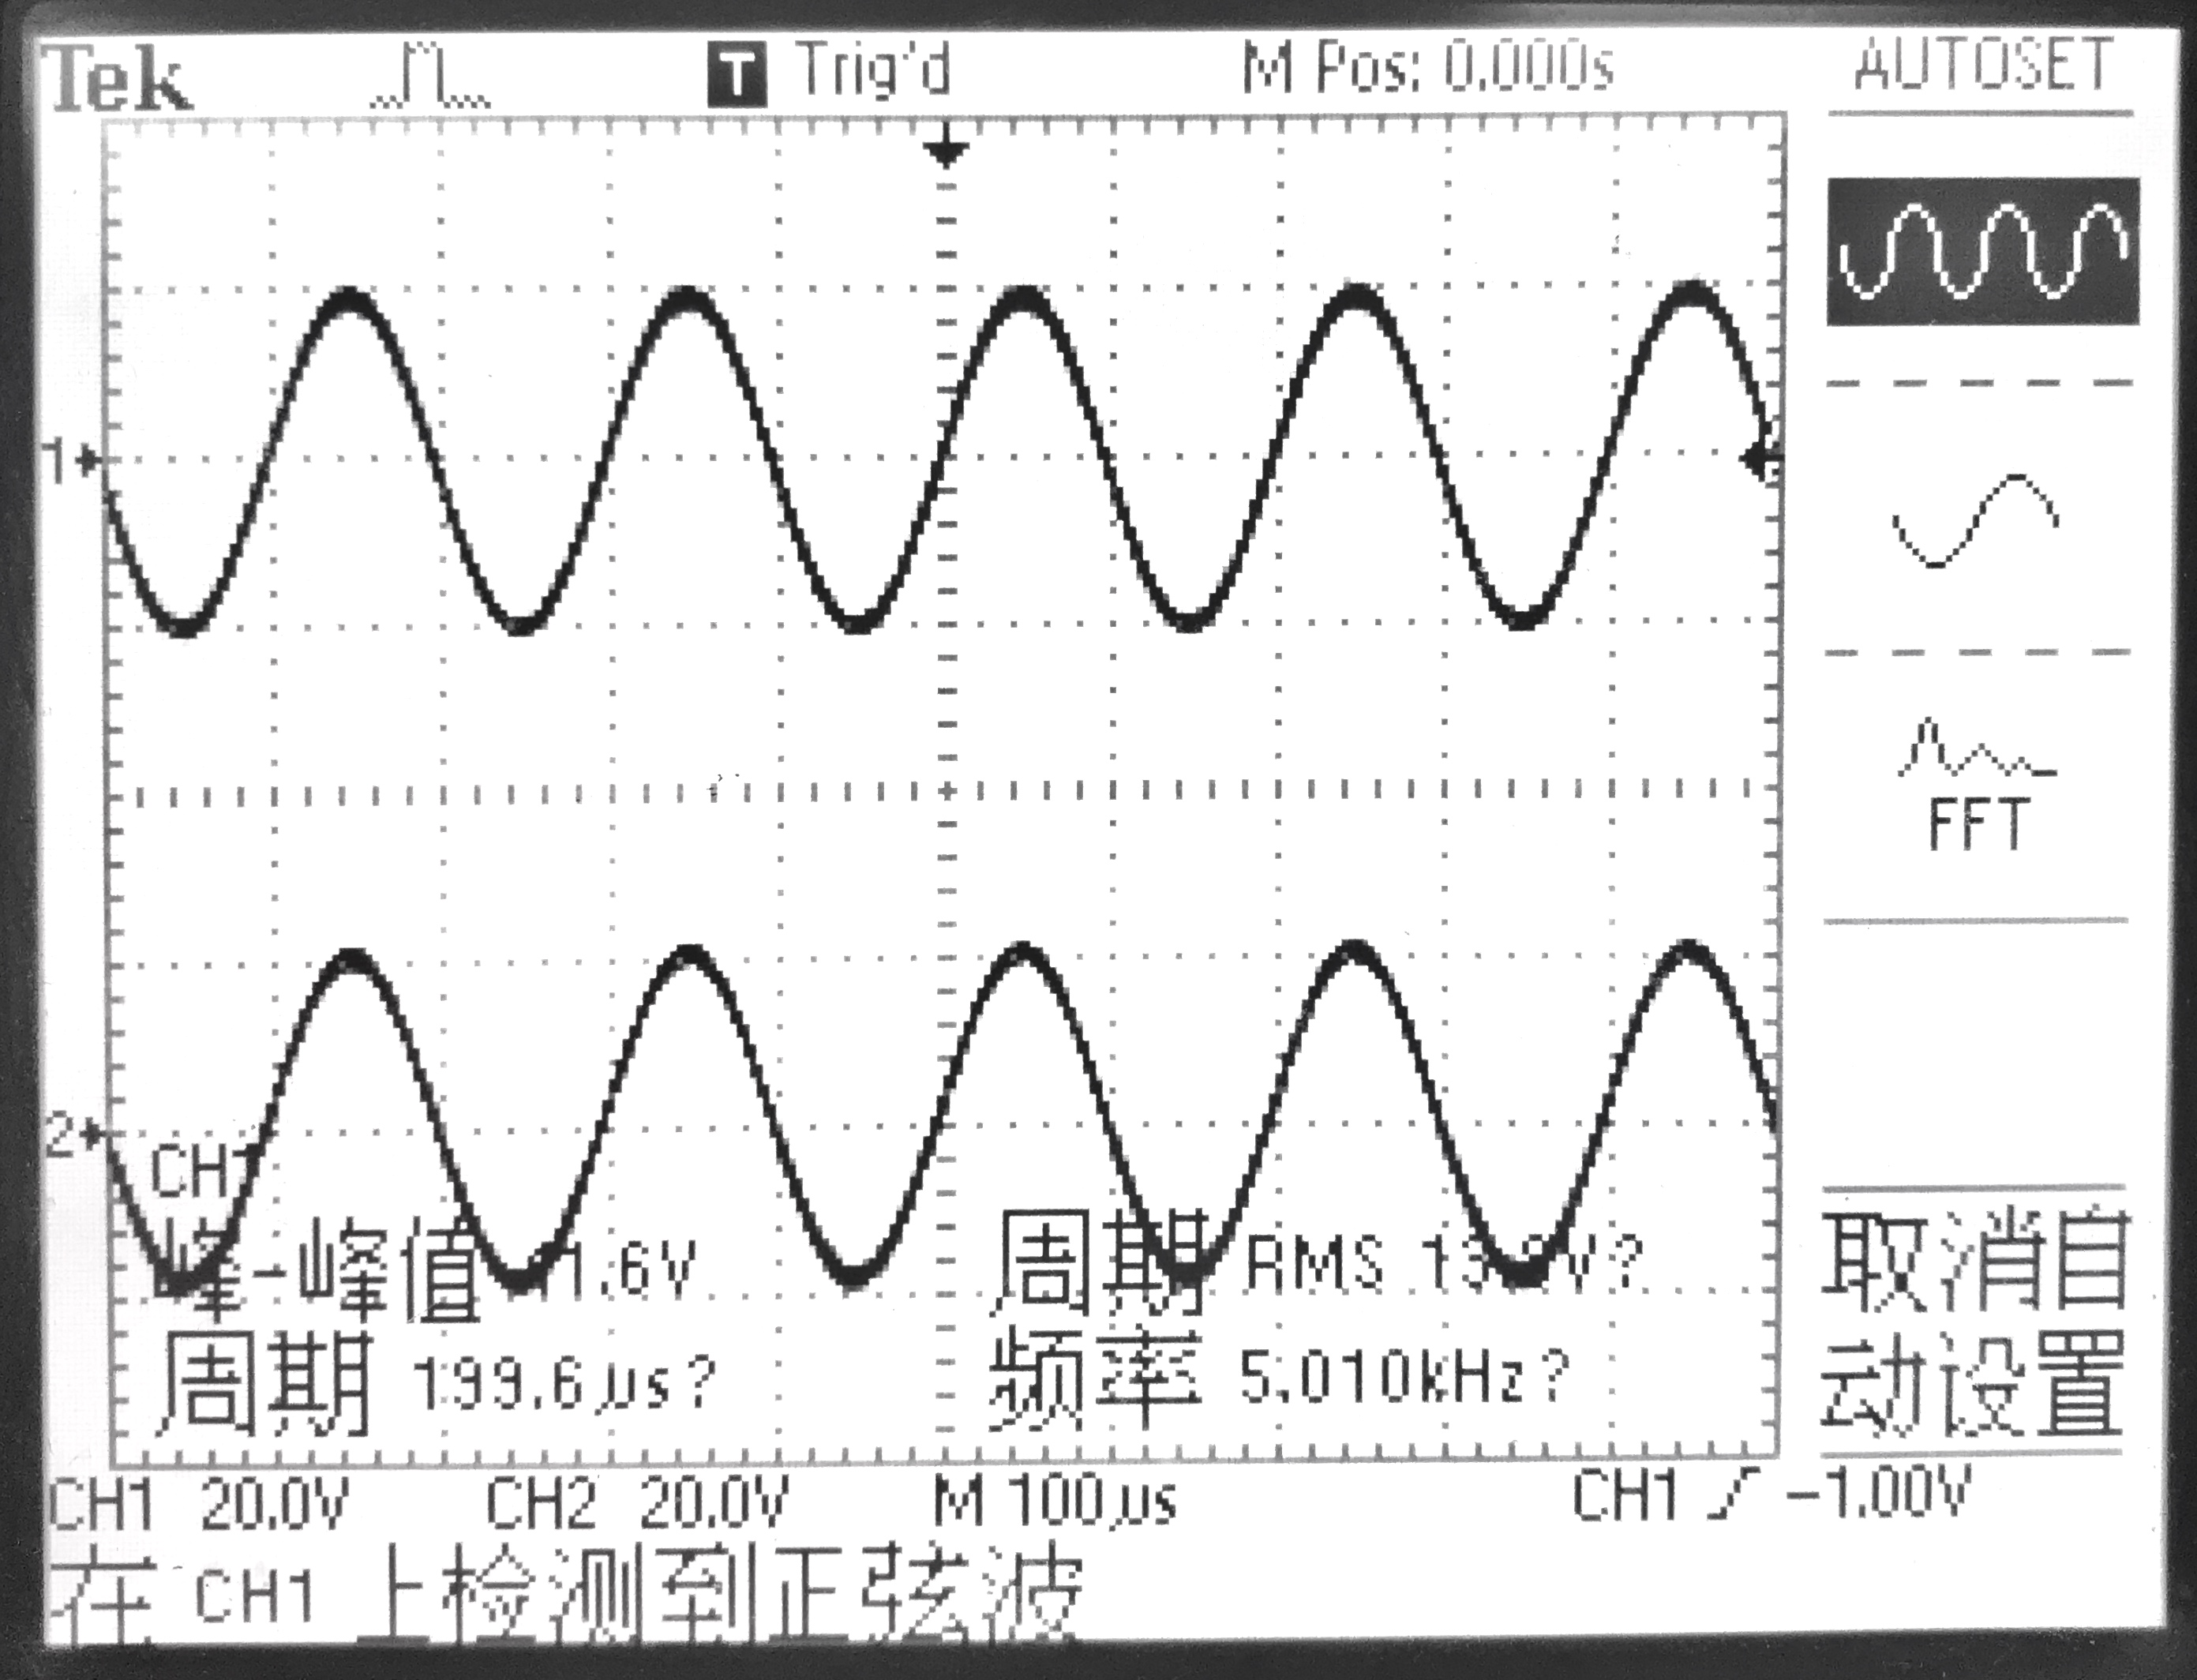
\includegraphics[width=10cm]{imp.jpg}
\caption{Directly comparing the waves by adjusting the vertical scale}
\end{figure}

\item After finding $U_R$, we should next find the corresponding $f$ for $U_R/\sqrt{2}$, to determine $f_1$ and $f_2$.
\item We can measure more data, especially in the first $T_{1/2}$ experiments, to reduce random errors.
\item All the measurements in this experiment is single-measurements. Thus, by repeating the procedure for multiple groups of same data, we get rid of random errors (But this will cause type-A uncertainty, which increase the uncertainty).
\end{itemize}



\newpage
\section{Reference}
\noindent [1] N. N. Bhargava $\&$ D. C. Kulshreshtha (1983). Basic Electronics and Linear Circuits. Tata McGraw-Hill Education. p.90. ISBN 978-0-07-451965-3. \\
\noindent [2] M. Krzyzosiak (2021). Exercise 5 - lab manual [rev. 2.6].pdf (UMJI-SJTU, Shanghai). \\
\noindent [3] "The Physics Of Resonance". Intuitor.com (1994-2016).10 July 2017. Web. 3 Dec. 2021. $<$\url{http://www.intuitor.com/resonance/circuits.html}$>$


\newpage
\section*{APPENDIX - DATA SHEET}

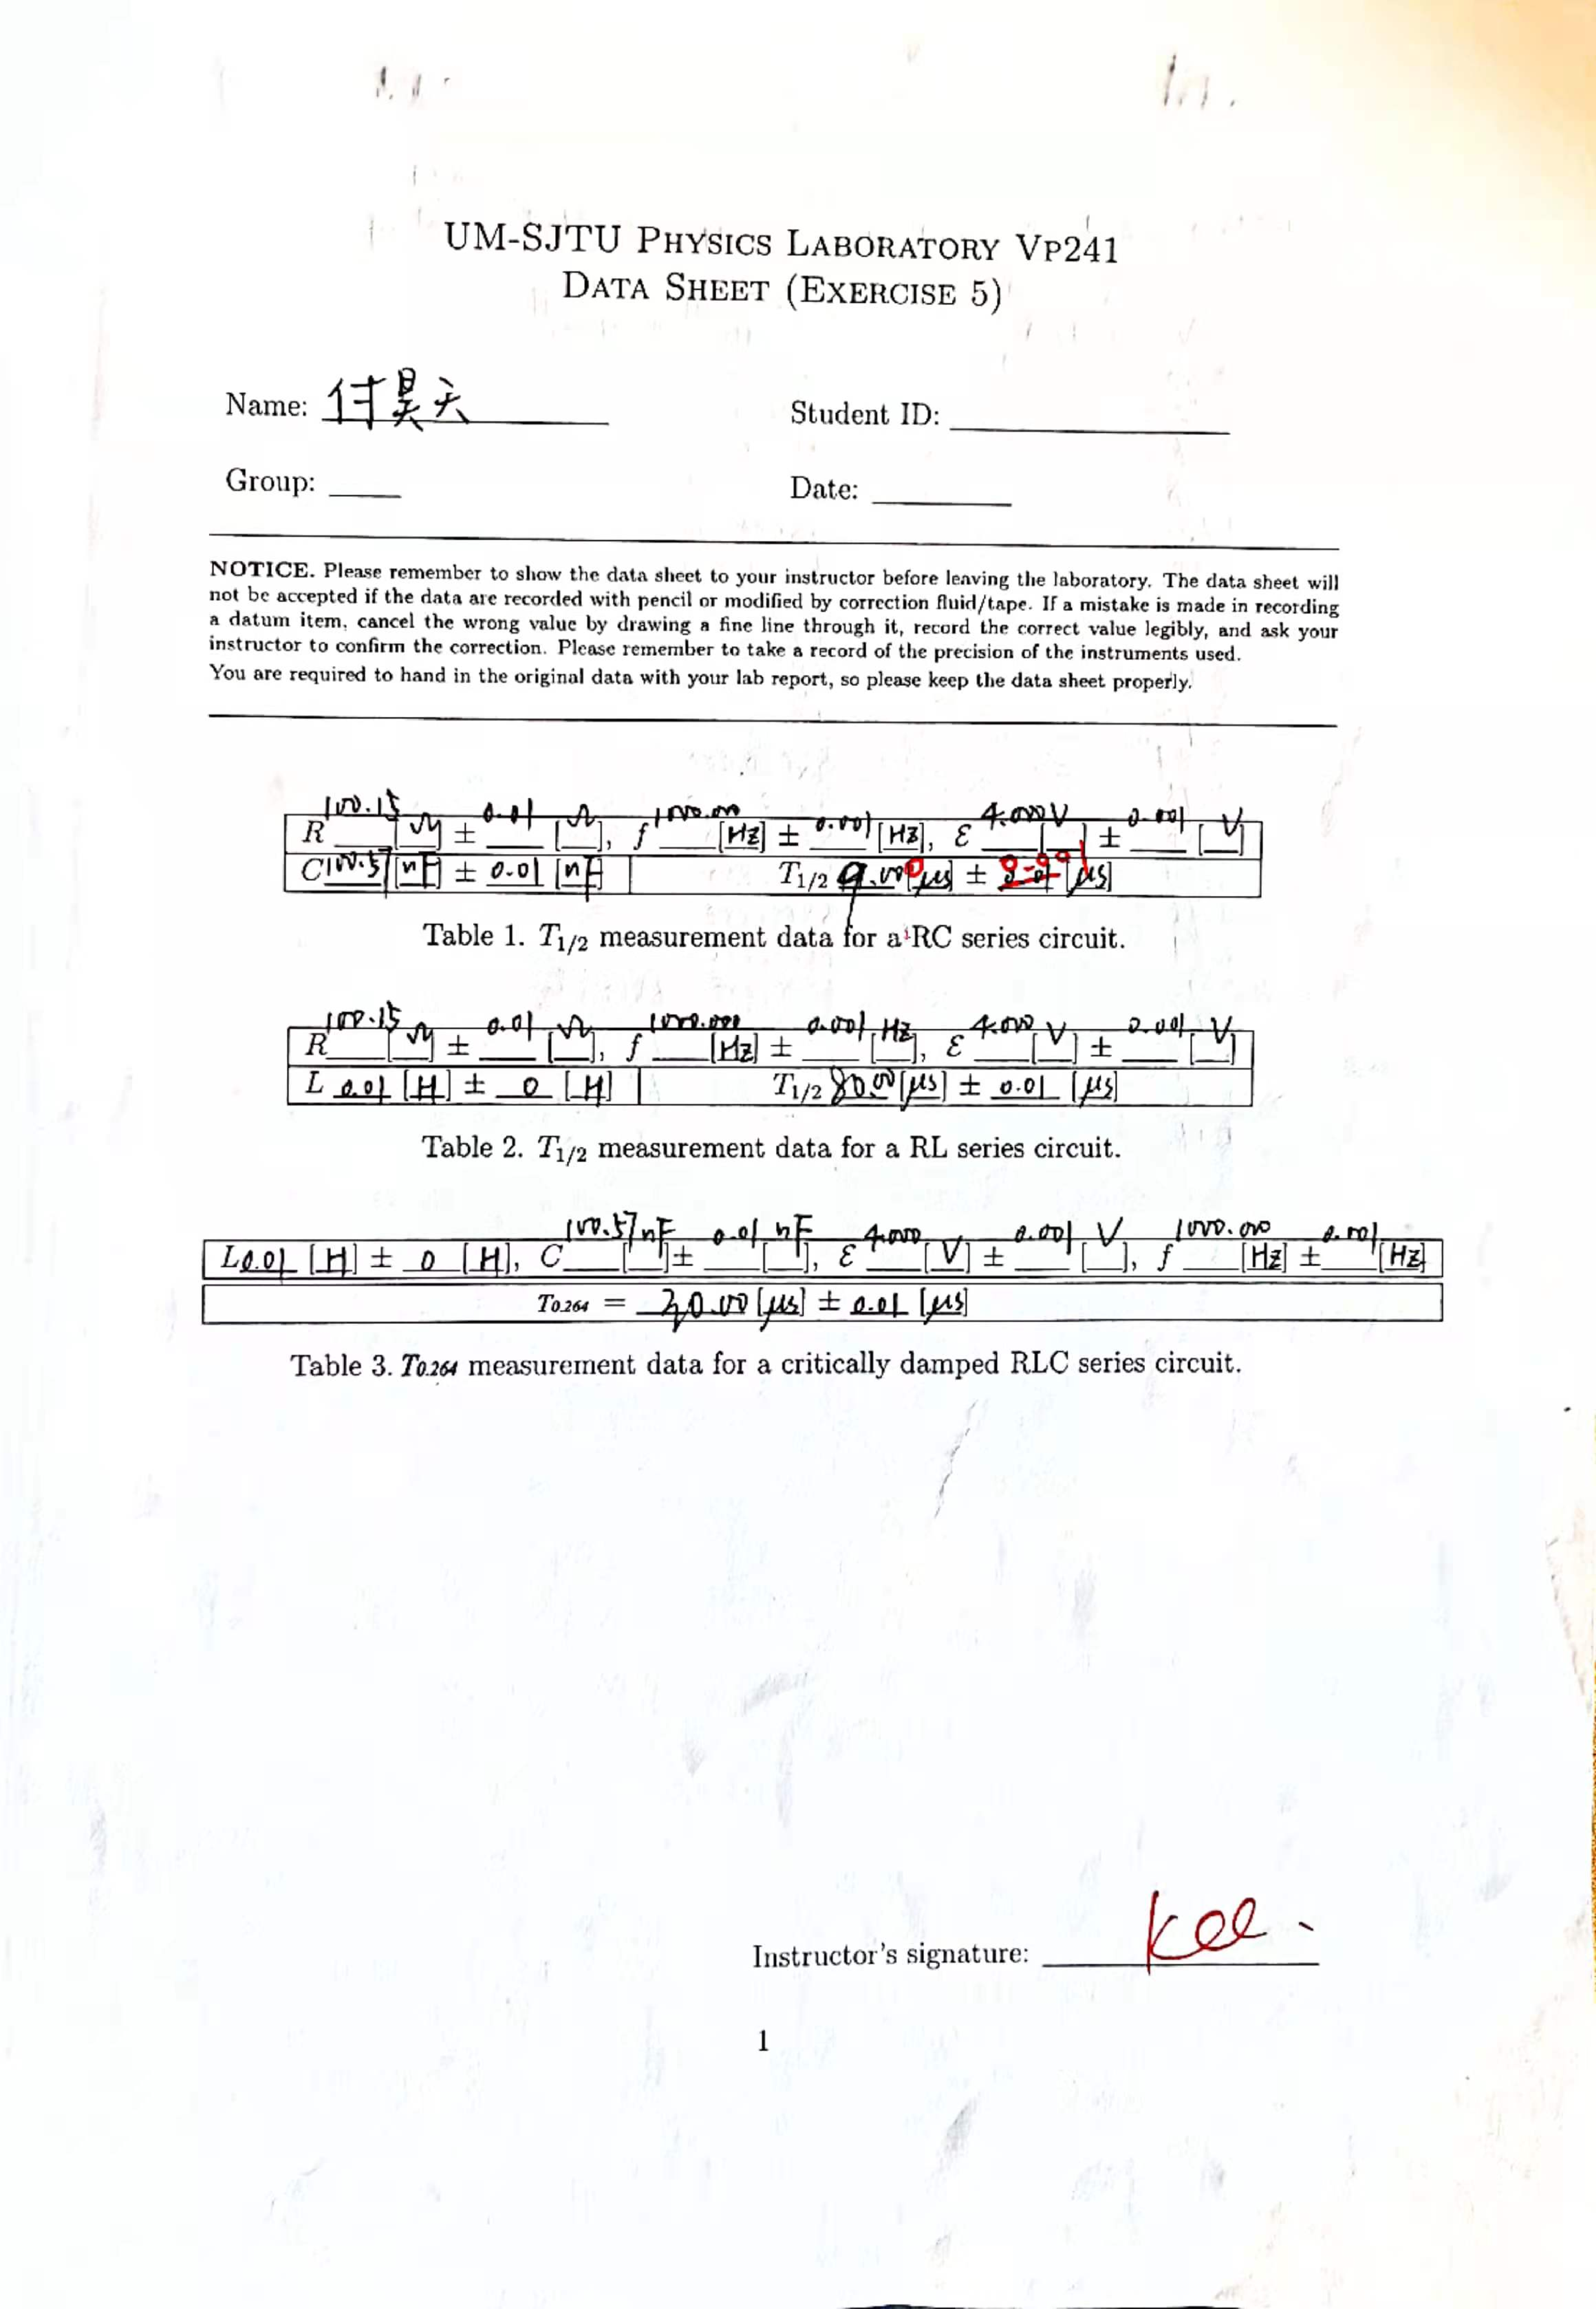
\includepdf{data_sheet1.pdf}
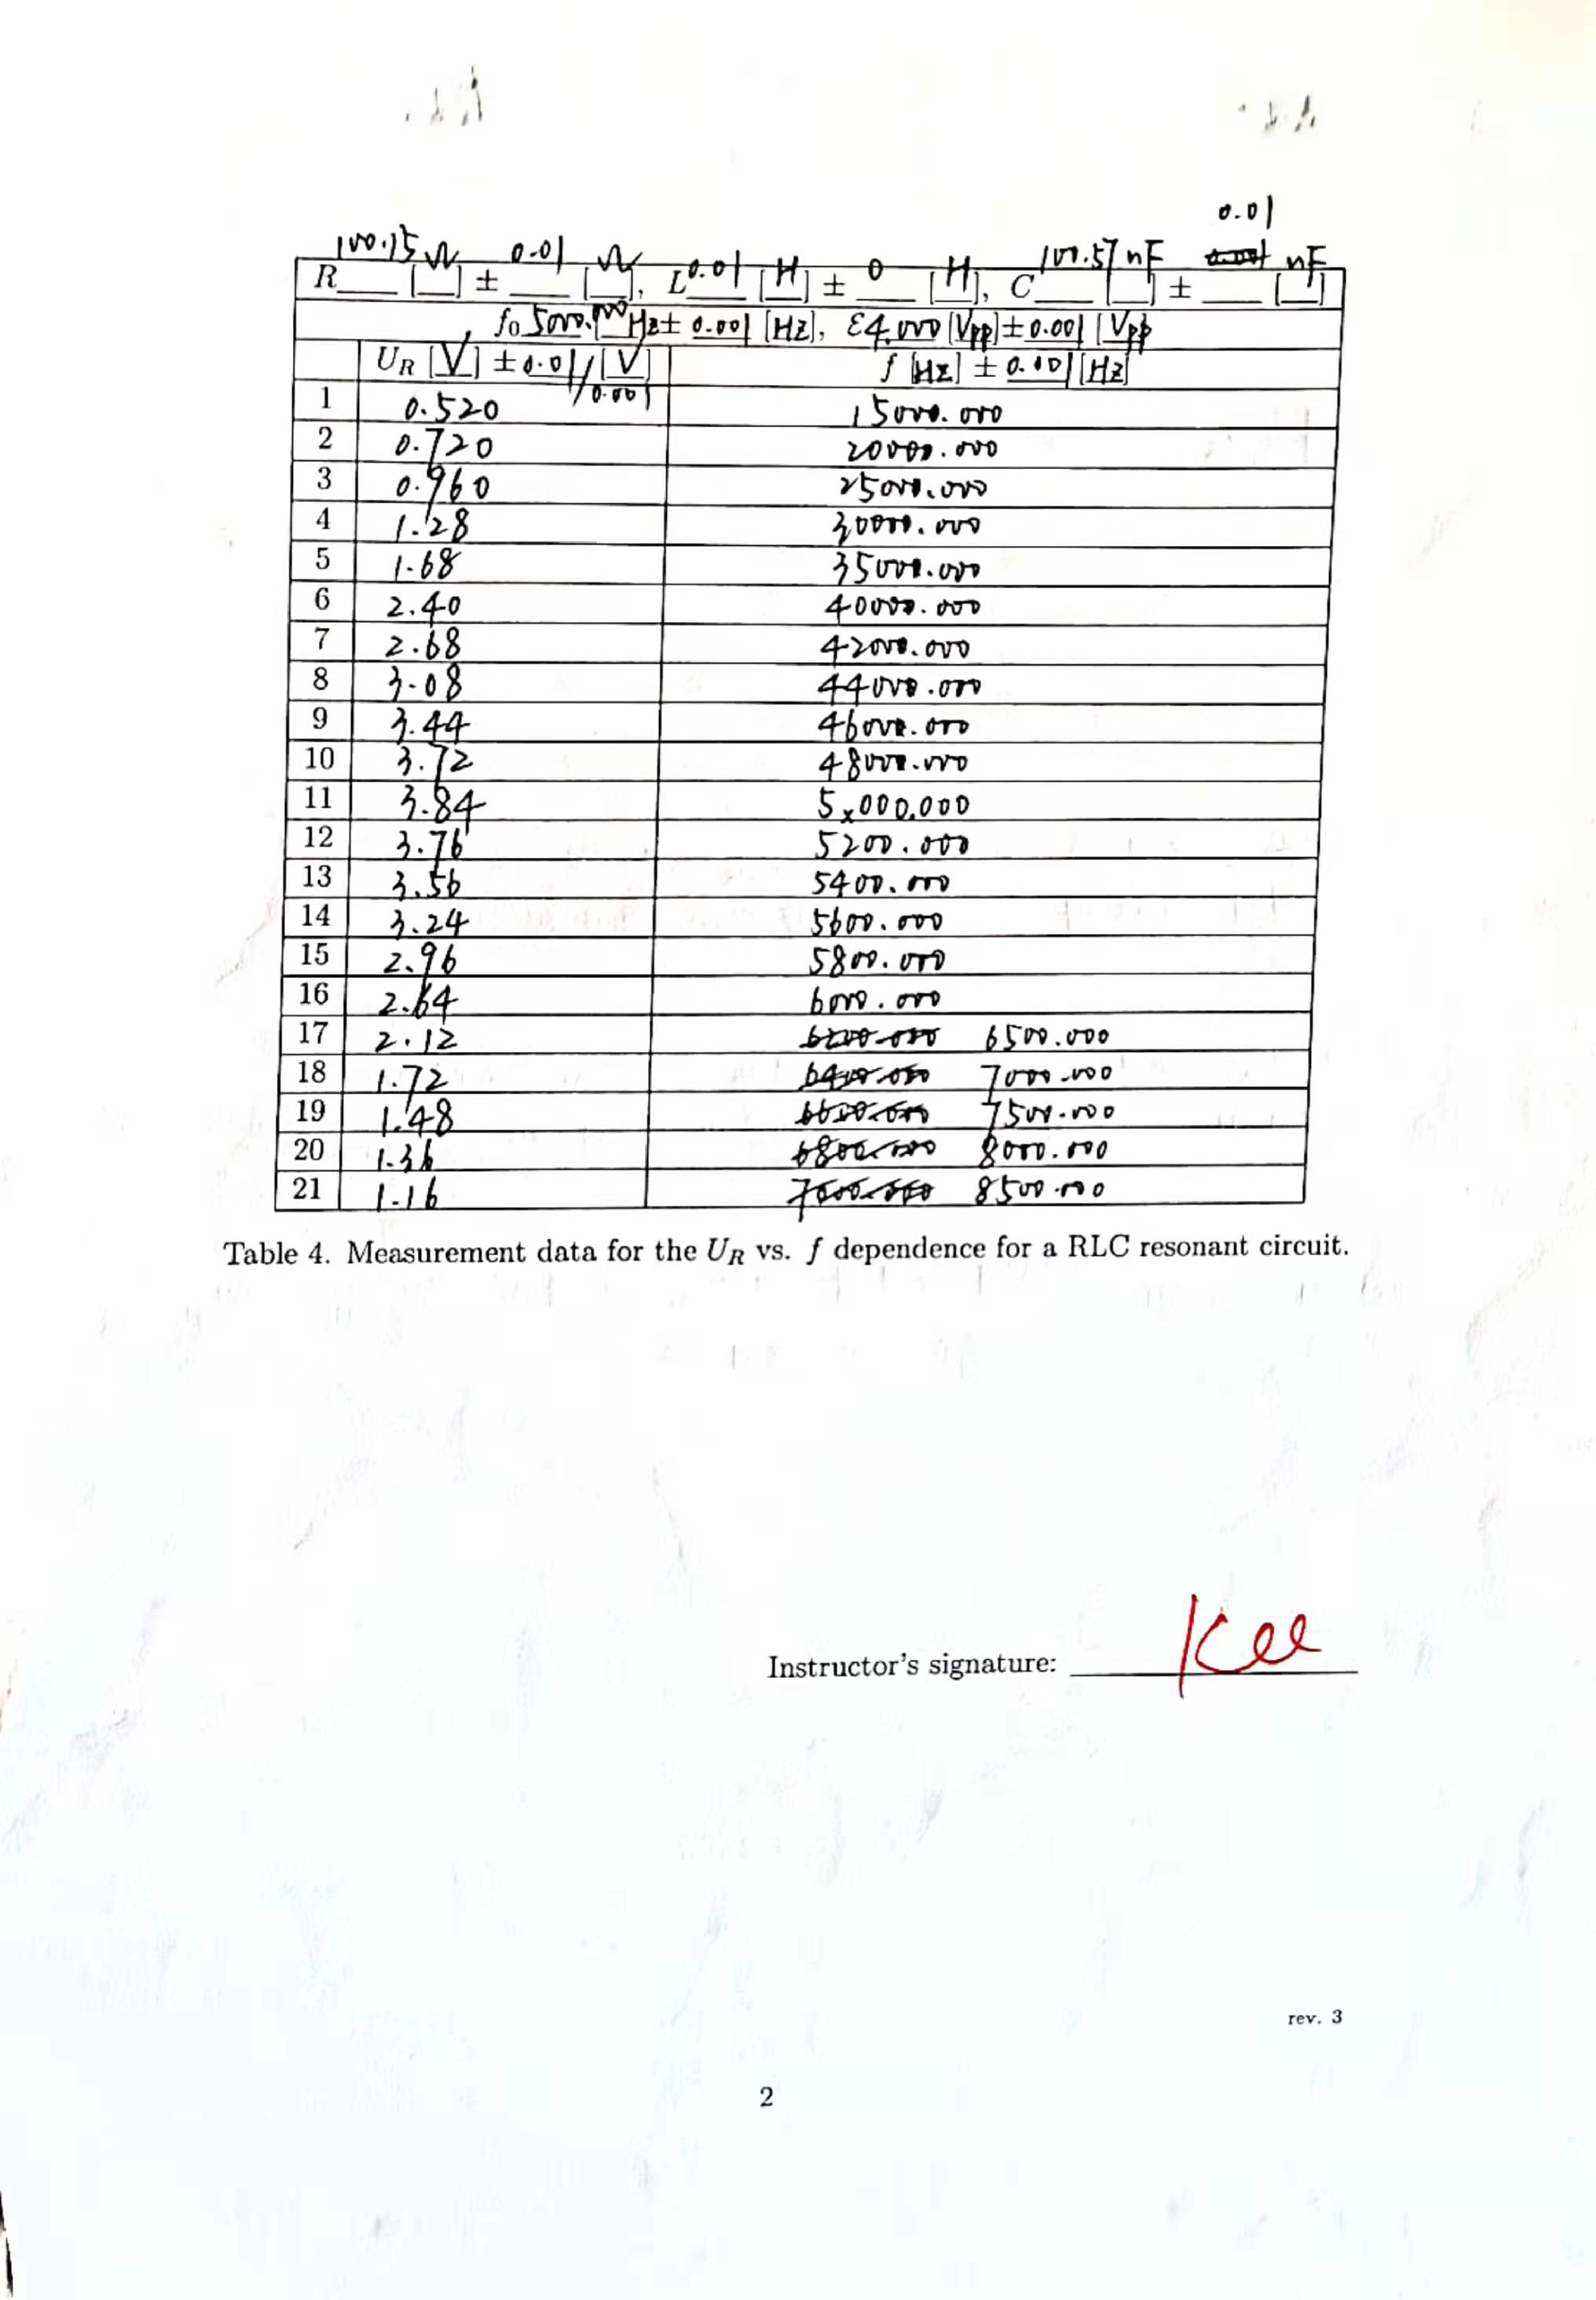
\includepdf{data_sheet2.pdf}

\end{document}
